\documentclass[12pt,oneside]{book}
\usepackage{times,mathptmx}
\usepackage[pdftex]{graphicx}
\usepackage{calc}
\usepackage{tabularx,ragged2e,booktabs,caption,subcaption}
\usepackage{array}
\newcolumntype{L}[1]{>{\raggedright\let\newline\\\arraybackslash\hspace{0pt}}m{#1}}
\newcolumntype{C}[1]{>{\centering\let\newline\\\arraybackslash\hspace{0pt}}m{#1}}
\newcolumntype{R}[1]{>{\raggedleft\let\newline\\\arraybackslash\hspace{0pt}}m{#1}}
\usepackage{multirow}
\usepackage{tocloft}
\usepackage{xcolor}
\usepackage{color,soul}
\usepackage{amsmath}
\definecolor{linknavy}{rgb}{0,0,0.50196}
\definecolor{linkred}{rgb}{1,0,0}
\definecolor{linkblue}{rgb}{0,0,1}
\usepackage{float}
\usepackage{graphpap}
\usepackage{rotating}
\usepackage{graphicx}
\usepackage{geometry}
\usepackage{relsize}
\usepackage{ltablex}
\usepackage{longtable}
\usepackage{lscape}
\usepackage{amssymb}
\usepackage{makeidx} % Create index at end of document
\usepackage[nottoc,notlof,notlot]{tocbibind} % Put the bibliography and index in the ToC
\usepackage{lastpage} % Automatic last page number reference.
\usepackage[T1]{fontenc}
\usepackage{enumerate}
\usepackage{upquote}
\usepackage{moreverb}
\usepackage{xfrac}
\usepackage{cite}
\usepackage{tikz}
% \usepackage{subfig}
% \usepackage{caption}
\usepackage[toc,page]{appendix}
\usepackage{notoccite}
\usepackage{colortbl}
\usepackage{titlesec}
\titleformat{\chapter}[hang] 
{\normalfont\huge\bfseries}{\chaptertitlename\ \thechapter}{1em}{} 
\titlespacing*{\chapter}{0pt}{-30pt}{20pt}

\newcommand{\nopart}{\expandafter\def\csname Parent-1\endcsname{}} % To fix table of contents in pdf.

\usepackage{siunitx}
\sisetup{
    detect-all = true,
    input-decimal-markers = {.},
    input-ignore = {,},
    inter-unit-product = \ensuremath{{}\cdot{}},
    multi-part-units = repeat,
    number-unit-product = \text{~},
    per-mode = fraction,
    separate-uncertainty = true,
}

\usepackage{listings}
\usepackage{textcomp}
\definecolor{lbcolor}{rgb}{0.96,0.96,0.96}

\usepackage[pdftex,
        colorlinks=true,
        urlcolor=linkblue,     % \href{...}{...} external (URL)
        citecolor=linkred,     % citation number colors
        linkcolor=linknavy,    % \ref{...} and \pageref{...}
        pdfproducer={pdflatex},
        pdfpagemode=UseNone,
        bookmarksopen=true,
        plainpages=false,
        verbose]{hyperref}

\setlength{\textwidth}{6.5in}
\setlength{\textheight}{9.0in}
\setlength{\topmargin}{0.in}
\setlength{\headheight}{0.pt}
\setlength{\headsep}{0.in}
\setlength{\parindent}{0.0in}
\setlength{\itemindent}{0.25in}
\setlength{\oddsidemargin}{0.0in}
\setlength{\evensidemargin}{0.0in}
% \setlength{\leftmargini}{\parindent} % Controls the indenting of the "bullets" in a list
\setlength{\cftsecnumwidth}{0.45in}
\setlength{\cftsubsecnumwidth}{0.5in}
\setlength{\cftfignumwidth}{0.45in}
\setlength{\cfttabnumwidth}{0.45in}
\setlength{\parskip}{1em}

\newcommand{\titlesigs}
{
\large
\flushright{UL Firefighter Safety Research Institute\\
{\em Stephen Kerber, Director} \\
\hspace{1in} \\
}
}

\newcommand{\headerB}[1]{
\flushleft{
\fontsize{28}{33.6}\selectfont
\bf{#1}
}
}

\newcommand{\headerC}[1]{
\vspace{.5in}
\flushright{\fontsize{14}{16.8}\selectfont
#1}
}

% \newcolumntype{L}{>{\centering\arraybackslash}m{4cm}}

\floatstyle{boxed}
\newfloat{notebox}{H}{lon}
\newfloat{warning}{H}{low}

\newenvironment{conditions}
  {\par\vspace{\abovedisplayskip}\noindent\begin{tabular}{>{$}l<{$} @{${}={}$} l}}
  {\end{tabular}\par\vspace{\belowdisplayskip}}


% Rename chapter headings
\renewcommand{\chaptername}{}
\renewcommand{\bibname}{References}

\usepackage{fancyhdr}
\pagestyle{fancy}
\lhead{}
\rhead{}
\chead{}
\renewcommand{\headrulewidth}{0pt}

% UN COMMENT TO PLACE WATERMARK
\usepackage{draftwatermark}
\SetWatermarkText{DRAFT}
\SetWatermarkScale{1}

\usepackage{subcaption}
\usepackage{xfrac}

\begin{document}
\pagenumbering{gobble}

\bibliographystyle{unsrt}
%\pagestyle{empty}

\begin{minipage}[t][9in][s]{6.25in}


\headerB{
Impact of Fire Attack Utilizing \\
Interior and Exterior Streams on\\ 
Firefighter Safety and Occupant \\
Survival: Full Scale Experiments\\
}

\normalsize

\headerC{
{
\flushleft{
Robin Zevotek \\
Keith Stakes \\
Joseph Willi
\vspace{0.2in}
UL Firefighter Safety Research Institute \\
Columbia, MD 21045 \\
\vspace*{2\baselineskip}

}

\vfill

\flushright{


\includegraphics[width=2.in]{Figures/General/FSRI_GraphicShield} \\[.3in]
}
}
}

\end{minipage}

\newpage
\hspace{5in}
\newpage

\frontmatter

\begin{minipage}[t][9in][s]{6.25in}
\pagenumbering{gobble}


\headerB{
Impact of Fire Attack Utilizing \\
Interior and Exterior Streams on\\ 
Firefighter Safety and Occupant \\
Survival: Full Scale Experiments\\
}

\headerC{
\flushleft{
Craig Weinschenk \\
Keith Stakes \\
Robin Zevotek \\
\vspace{0.2in}
{UL Firefighter Safety Research Institute \\
Columbia, MD 21045 \\}}

\flushleft{\today \\}
}


\vfill

\flushright{
\includegraphics[width=2in]{Figures/General/FSRI_GraphicShield}}

\titlesigs

\end{minipage}

\frontmatter

\pagestyle{plain}
\pagenumbering{roman}

\begin{minipage}[t][9in][s]{6.25in}

\flushleft{In no event shall UL be responsible to anyone for whatever use or non-use is made of the information contained in this Report and in no event shall UL, its employees, or its agents incur any obligation or liability for damages including, but not limited to, consequential damage arising out of or in connection  with the use or inability to use the information contained in this Report. Information conveyed by this Report applies only to the specimens actually involved in these tests. UL has not established a factory Follow-Up Service Program to determine the conformance of subsequently produced material, nor has any provision been made to apply any registered mark of UL to such material. The issuance of this Report in no way implies Listing, Classification or Recognition by UL and does not authorize the use of UL Listing, Classification or Recognition Marks or other reference to UL on or in connection with the product or system.
}

\vspace{3in}


\vfill

\hspace{1in}

\end{minipage}

\newpage

\chapter*{\centering Acknowledgments}
	
This work was funded through a grant from the Department of Homeland Security's Assistance to Firefighters Grant Program under the Fire Prevention and Safety Grants: Research and Development. Without this critical funding and support, this vital fire service research would not be possible.

\vspace*{\baselineskip}

\begin{center}
	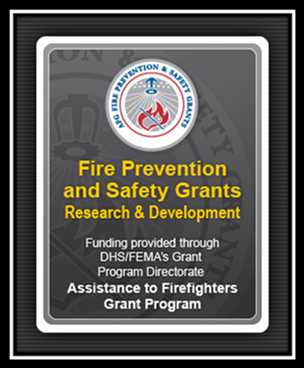
\includegraphics[width=0.28\textwidth]{Figures/General/DHS}
\end{center}

\clearpage

To assist the design and implementation of the experiments for the Fire Attack study, fire service experts were gathered from across the world with knowledge in fire suppression and the impact of interior and exterior fire streams. The individuals below provided direction for the project, assisting in planing the experiments, witnessing the testing, and developing concrete conclusions. Their tireless support and effort make this project relevant to the fire service across the world. 

% \begin{table}[!ht]
% 	\centering
% 	\caption*{Fire Service Technical Panel}
% 	\begin{tabular}{ll}
% 		\toprule[1.5pt]
% 		Name & Fire Department \\ 
% 		\midrule
% 		Steve Brisebois  & Montreal Fire Department \\ 
% 		Matt Carrigan    & Montgomery County Fire and Rescue Service \\ 
% 		Tony Carroll     & Washington DC Fire Department \\ 
% 		Albert Castillo  & Houston Fire Department \\ 
% 		Chad Christensen & Los Angeles County Fire Department \\ 
% 		John Chubb       & Dublin Fire Brigade \\ 		 		  
% 		Danny Doyle      & Pittsburgh Fire Department \\ 
% 		Aaron Fields     & Seattle Fire Department \\ 
% 		Jason Floyd      & Las Cruces Fire Department \\ 
% 		John Gallagher   & Boston Fire Department \\ 
% 		Chad Green       & Anchorage Fire Department \\ 
% 		Kelly Hanink     & Eden Prairie Fire Department \\ 
% 		Samuel Hittle    & Wichita Fire Department \\ 
% 		Jacob Hoffman    & Toledo Fire/Rescue Department \\ 
% 		Josh Hummel      & Howard County Department of Fire and Rescue Services \\ 
% 		Jerry Knapp      & West Haverstraw (NY) Fire Department \\ 
% 		Dennis Legear    & Oakland Fire Department (Ret.) / LEFD Consulting\\ 
% 		Hans Neiling     & Zuid Limburg Fire \\ 
% 		Nick Martin      & Columbia Fire Department \\ 
% 		Ray McCormack    & Fire Department of New York \\ 
% 		John McDonough   & New South Wales Fire Department \\ 
% 		Jordan Mohr      & Sedgwick County Fire District 1 \\ 
% 		Steve Pegram     & Goshen Township Fire and EMS \\ 
% 		\bottomrule[1.25pt]
% 	\end{tabular}
% \end{table}

\begin{table}[!ht]
	\centering
	\caption*{Fire Service Technical Panel}
	\begin{tabular}{|l|l|}
		\hline
		Name & Fire Department \\ 
		\hline \hline
		Steve Brisebois  & Montreal Fire Department \\ \hline
		Matt Carrigan    & Montgomery County Fire and Rescue Service \\ \hline
		Tony Carroll     & Washington DC Fire Department \\ \hline
		Albert Castillo  & Houston Fire Department \\ \hline
		Chad Christensen & Los Angeles County Fire Department \\ \hline
		John Chubb       & Dublin Fire Brigade \\ \hline	 		  
		Danny Doyle      & Pittsburgh Fire Department \\ \hline
		Aaron Fields     & Seattle Fire Department \\ \hline
		Jason Floyd      & Las Cruces Fire Department \\ \hline
		John Gallagher   & Boston Fire Department \\ \hline
		Chad Green       & Anchorage Fire Department \\ \hline
		Kelly Hanink     & Eden Prairie Fire Department \\ \hline
		Samuel Hittle    & Wichita Fire Department \\ \hline
		Jacob Hoffman    & Toledo Fire/Rescue Department \\ \hline
		Josh Hummel      & Howard County Department of Fire and Rescue Services \\ \hline
		Jerry Knapp      & West Haverstraw (NY) Fire Department \\ \hline
		Dennis Legear    & Oakland Fire Department (Ret.) / LEFD Consulting \\ \hline
		Hans Neiling     & Zuid Limburg Fire \\ \hline
		Nick Martin      & Columbia Fire Department \\ \hline
		Ray McCormack    & Fire Department of New York \\ \hline
		John McDonough   & New South Wales Fire Department \\ \hline
		Jordan Mohr      & Sedgwick County Fire District 1 \\ \hline
		Steve Pegram     & Goshen Township Fire and EMS \\ \hline
	\end{tabular}
\end{table}

The authors would also like to acknowledge the UL LLC technical support staff for their assistance in conducting the full-scale fire experiments.

\cleardoublepage
\phantomsection
\addcontentsline{toc}{chapter}{Contents}
\tableofcontents

\cleardoublepage
\phantomsection
\addcontentsline{toc}{chapter}{List of Figures}
\listoffigures

\cleardoublepage
\phantomsection
\addcontentsline{toc}{chapter}{List of Tables}
\listoftables

\chapter{List of Acronyms}

\begin{tabbing}
\hspace{1.5in} \= \\
AFG \> Assistance to Firefighters Grant program  \\
DHS \> U.S Department of Homeland Security   \\   
FEMA \> Federal Emergency Management Agency  \\
NFPA \> National Fire Protection Association \\
SB \> Smooth Bore \\
SS \> Straight Stream \\
NF \> Narrow Fog \\
UL FSRI \> UL Firefighter Safety Research Institute \\
USFA \> United States Fire Administration  \\
\end{tabbing}

\newpage

\mainmatter

\chapter*{Abstract}

As research continues into how fire department interventions affect fire dyanmics in the modern fire environment; questions continue to arise on the impact and implications of interior versus exterior fire attack on both firefighter safety and occupant survivability. Previous research into various types of fire ground ventilation, flow paths, and exterior fire streams has provided the fire service with a more in-depth understanding of fire dynamics in addition to raising questions about certain fire attack methods stemming from differing traditions and myths. This knowledge gap and lack of previous research into the impact of fire streams has driven the need for further research into fire department interventions at structure fires with a focus on hose streams and suppression tactics. Statistics show that both firefighters and building occupants continue to loose their lives due to fire. As such, research into the various methods of fire attack will allow a broader understanding of how firefighter interventions on the fire ground can impact the outcome of both life safety and property protection. 

This study will build and expand upon the fire research conducted to date by analyzing how firefighting tactics, specifically suppression methods, affect the thermal exposure and survivability of both firefighters and buidling occupants in addition to impacting fire behavior in structures. The project will be comprised of 3 parts:

\vspace*{\baselineskip}
\begin{itemize}
	\item Part I: Water Distribution.
	\item Part II: Air Entrainment
	\item Part III: Full-Scale Residential Fire Experiments.
	\end{itemize}
\vspace*{\baselineskip}

\newpage

\tableofcontents

\newpage

\chapter*{Introduction}

The purpose of this study is to improve firefighter safety, fireground tactics, and the knowledge of fire dynamics by providing the fire service with credible scientific information on the impacts and implications of interior and exterior fire attack that is obtained from the results of water flow and full-scale fire testing in representative single family homes. Part I of the study is aimed at determining how water is distributed within a compartment, and Part II of the study attempts to quantify air entrainment by hose streams to provide insight into how different application methods; nozzle types and patterns; pressures/flows; and stream location and angle combinations move air inside buildings. Parts I and II were conducted without the presence of fire to gain a basic understanding of air flow and water flow before full-scale fire experiments were conducted during Part III of the study. These full-scale fire experiments were designed based on the results from Parts I and II of the study. 

\clearpage

\chapter{Background}

Recent fire service research has highlighted the importance of applying water to the fire as quickly as possible. This tactical consideration has highlighted a knowledge gap and increased the interest in better understanding the impact of water applied as part of an interior attack or exterior attack. Many variables exist in fire attack that impact firefighter effectiveness and victim survivability, including stream placement, the timing required to get water on the fire, stream type, stream movement, air entrainment, steam development, position of flow paths, and hot gas cooling and contraction. The fire service's most important tool for many years at structure fires is their hose line, however many questions have arisen as more research shows the impact of ventilation, flow paths and exterior fire streams. Whether a fire attack crew chooses to apply water as part of an interior attack or as part of an exterior or transitional attack they need to know what impact their stream has on the fire environment ahead of them. This is difficult on the fire ground because visibility is commonly limited and therefore all of their experience is from behind the nozzle. This results in beliefs about conditions (e.g., temperature), ahead of the nozzle and its impact on victim survivability but knowledge of actual impact has not been researched. Additionally, when the fire is ultimately suppressed that does not mean it was done most effectively, efficiently and safely but the experience gained suggests that it was. Fire service adages such as ``don’t put water on smoke,'' ``you will steam the victims,'' and ``fog nozzles always disrupt the thermal layer'' have been passed on from generation to generation with little context or substantiation. Without the context these concepts get treated like rules and can severely limit firefighters understanding of fire suppression.

Fire training curriculum defines 3 fire attack methods, direct attack, indirect attack and combination attack. Direct attack involves the discharge of water directly onto the burning fuel. Indirect attack involves directing the stream toward the ceiling of a compartment in order to generate a large amount of steam in order to cool the compartment. Converting the water to steam displaces oxygen, absorbs the heat of the fire and cools the hot gas layer sufficiently for firefighters to safely enter and make a direct attack. Combination attack extinguishes a fire by using both a direct and indirect attack. Another technique to safely approach a fire that cannot be reached with a direct attack is gas cooling. Gas cooling provides a buffer zone around the attack team but the larger the compartment the less the impact on cooling the hot gas layer. Gas cooling must be a continuous process while advancing toward a shielded fire. Techniques for effective gas cooling and the upper limit of the volume where gas cooling is effective is not well known.  

In fire fighter training there is a lot of emphasis on steam generation but little is taught or demonstrated about the mechanics of suppression. Water vaporized in the upper gas layer reduces the total volume of the hot gases and steam. Water vaporized on hot surfaces such as the ceiling does not take much energy from the fire and therefore the volume of steam produced lowers the upper layer and makes conditions less tenable. These concepts are very important when the fire is not able to be directly attacked by applying water on burning fuel but is very difficult to visualize during a fire attack with limited visibility. Many of these fire suppression concepts are difficult to learn and refine because realistic ventilation limited fires are not safely replicated in firefighter training structures. Conditions created by todays fuels with heat release rates and smoke production properties commonly found in our structures are not allowed when following fire service training standards. Therefore the impact of hose streams in concrete training structures or metal containers can be misleading to firefighters resulting in incorrect inferences. This may then lead to inappropriate fire ground tactics with potentially deadly results. Research is needed to better understand the impact of hose streams so that proper messages can be taught in fire service training programs.

There are potentially harmful effects of inappropriate water application regardless of the type of hose stream. Since firefighters today are more aware of the need to cool hot smoke (fuel) in the upper layer, it is essential to understand the capabilities and limitations of each type of stream. The impact of hose stream application as one advances during a fire attack is dependent on a number of factors, principle of which are the flow path and where the steam is produced (in the hot gas layer or on contact with hot surfaces). Continuous application is likely to result in more steam being produced than gas contraction in the hot gas layer. Without ventilation in front of the hose stream, this can result in a reduction in tenability. However, when victims or firefighters are not in the flow path, and ventilation is in front of the hose stream, a combination attack can be quite effective for fully developed fire conditions.

Fire suppression effectiveness and firefighter safety are not achieved by water flow rate alone, but by appropriate use of a given flow rate under specific fire ground conditions. A flow rate must meet the critical flow rate to extinguish a fire depending on the heat release rate and should be higher to reduce the time to extinguishment. Drastically exceeding the critical flow rate has less impact on time to extinguishment but has a significant impact on the total amount of water used. There is little data to support that dramatically exceeding the critical flow rate results in increased firefighter safety. It has been estimated that only 5 to 10 percent of water applied during fire attack contributes to extinguishment. It is difficult for firefighters to realize the the efficiency of various hose stream techniques due to poor visibility on the fireground. However, by developing data in realistic structures, fuel sources, and fire scenarios, important inferences may be developed relative to different hose stream techniques, and use of water.

\clearpage

\chapter{Objectives and Limitations}

\section {Objectives}

The purpose of this study was to provide the fire service with scientific based knowledge on the impact of interior and exterior fire attack tactics on firefighter safety and trapped occupants to improve training and decision making on the fire ground. This was accomplished with the completion of the following objectives:

\begin{itemize}
	\item Improve firefighter safety by increasing knowledge of fire behavior.
	\item Develop knowledge of water streams applied during an interior and exterior/interior fire attack and its impact on firefighter safety and victim survivability.
	\item Understand where water goes and how air flows during interior and exterior/interior fire attack utilizing common procedures and what that means to fire dynamics within a structure.
	\item Gain understanding of the impact of water streams depending on the volume of the fire compartment/structure.
	\item Advance the understanding of victim survivability in the modern fire environment by working with experts in the use of pig carcasses and rodents.
	\item Develop and implement a methodology to measure moisture content in the modern fire environmental conditions to answer fire service concerns.
	\item Bring the `Science to the Streets' by transferring science based tactical considerations founded on experimental results that can be incorporated into firefighting standard operating procedures.
	\end{itemize}

All five of the Technology \& Fire Service Science issues facing the fire service determined during the 2nd National Fire Service Research Symposium \cite{NFFF} were incorporated into this study.

\clearpage

% \section{Technical Plan}

% This study consisted of the following tasks shown in the figure below. Part I of the study details the specifics of the project related to the results from Tasks 7A and 7B. 

% \begin{itemize}

% \begin{figure}[H]
% 	\centering
% 	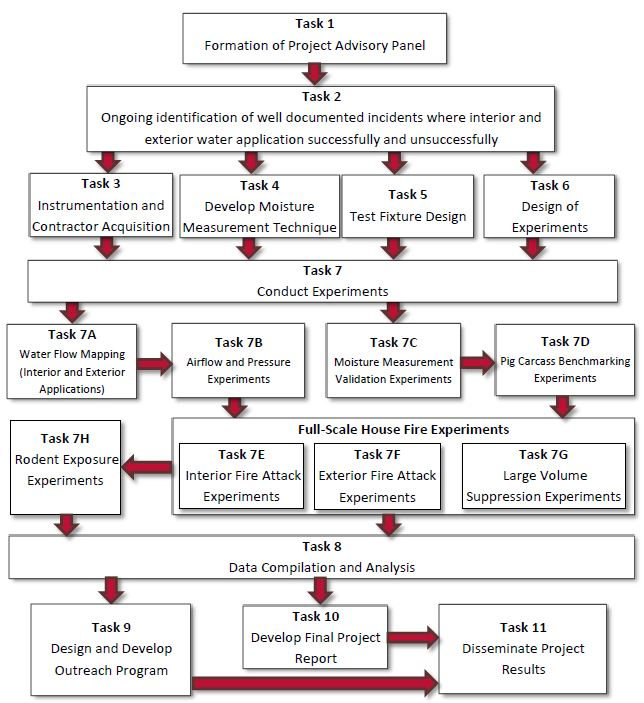
\includegraphics[width = 6in]{Figures/General/Flow_Chart}
% 	\caption{Project Technical Plan Flow Chart}
% 	\label{fig:TechPlanChart}
% \end{figure}

% \clearpage

% \item \textbf{Task 1 – Formation of a Project Advisory Panel}
% \normalfont
% \vspace*{\baselineskip}

% Task 1 will bring together an advisory panel of technical experts in the fire service; and fire service research field. An open application process will be administered to find fire service experts in fire stream application and training in fire attack methods. Representatives from organizations including: CFD (Chicago Fire Department), FDNY (Fire Department of New York), IAFC (International Association of Fire Chiefs), IAFF (International Association of Fire Fighters), NVFC (National Volunteer Fire Council), NIST (National Institute of Standards and Technology), and career and volunteer representatives from urban, suburban, and rural fire departments will be invited to participate. Invitations will also be extended to representatives of major fire service publications and training material publishers. This well rounded panel allows UL to ensure their research is directed to the target audiences and that the end product of the research is able to be easily disseminated into practice.
% \vspace*{\baselineskip}

% \item \textbf{Task 2 – Incident Review}
% \normalfont
% \vspace*{\baselineskip}

% Task 2 is to leverage our fire service advisory panel to conduct an extensive search to find examples of well documented successful and unsuccessful interior and exterior fire stream applications. This will be completed by monitoring fire service websites for videos and after action reports where there are defined flow paths and clear fire service fire attack actions. With approval of the fire department these incidents will be examined in detail to determine the impacts of fire stream type, flow, pattern and placement on the outcome of the incident, firefighter safety and victim injuries if applicable. Everyday the fire service is learning through their own experience and the experience of others through the means of sharing video. To make sure our experiments are tied in best with common fire service experiences we will identify trends in these incidents and tie the research results to the experience or beliefs gained from these incidents.
% \vspace*{\baselineskip}

% \item \textbf{Task 3 – Test Supplies, Instrumentation and Contractor Acquisition}
% \normalfont
% \vspace*{\baselineskip}

% Task 3 will allow for UL to acquire research supplies and instrumentation to complete this project. Instrumentation includes thermocouples to measure thermal conditions that potential victims or firefighters would be exposed to, differential pressure sensors and bidirectional probes to measure pressure and gas velocity throughout the test fixtures, bullet cameras to capture interior views of the test fixtures to provide visual evidence of conditions. Other test equipment such as data loggers, gas analyzers, thermal imaging cameras and video cameras were acquired from previous studies and will be utilized during this study. A contractor will also be selected to construct the test house structures using construction practices representative of what would be found in most neighborhoods across the country.
% \vspace*{\baselineskip}

% \item \textbf{Task 4 – Develop Moisture Measurement Technique}
% \normalfont
% \vspace*{\baselineskip}

% During this task different commercially available moisture measurement technologies will be examined for their ability to make moisture measurements in conditions that will be created in the full-scale house experiments. These conditions include elevated temperatures and a high density of particulate. This measurement will allow for the ability to map where steam travels in the structure to assess the impact of steam on fire victims and on fire service steam burns.

% Several well established instruments exist to characterize the environmental conditions within a structure containing fires by measuring a variety of effluent gases along with temperature, heat flux and flow characteristics. However, the ability to measure moisture content in conditions applicable to describing fire environments, particularly after water has been applied to suppress the fire, is not presently available. The effect of measuring moisture at elevated temperatures is critical for hazard assessments for both firefighters operating within a structure and potential victims who are trapped in the structure. In the SFPE Handbook, Purser suggests that:  “… it is possible that the presence of water vapor may be an important neglected hazard in fires”, and, “Humid air, steam or smoke with a high thermal capacity of latent heat (due to vapor content or suspended liquid or solid particles) may be dangerous at temperatures of around 212~$^{\circ}$F (100~$^{\circ}$C), causing burns throughout the respiratory tract. It may be possible to predict the likely effects of hot-smoke atmospheres if thermal capacity or latent heat were measured.” 

% Thus, the ability to measure moisture concentration in such environments is a critical avenue of research for firefighter safety as well as to fully understand the impact of tactical decisions on trapped victim safety. It is of particular importance to know the moisture content in the rooms adjacent to the fire room at the level of occupants crawling on the floor (1~ft above the floor) or on furnishings (3~ft above the floor). Based on past experimental results, the temperatures observed at these levels in rooms adjacent to the fire room are typically under 400~$^{\circ}$F.  

% Commercially available moisture sensors have been developed recently for industrial process control, but these have not been studied for applicability to the live fire conditions. At the University of Illinois, Professor Dimitrios Kyritsis’ lab has advanced multiple techniques based on electrical and laser based measurements of gases during internal combustion engine operation that can be adapted to the sooty, dynamically changing live-fire environment. While there are a large number of techniques to measure moisture, most are inapplicable to the situation of high temperature moisture measurements in a combusting environment. Two techniques that could have use in these types of environments are infrared absorption techniques and electrical impedance techniques. There are two different methods to measure moisture using electrical impedance, resistive methods and capacitive methods. Both methods measure the relative humidity of the environment. Each method has its own set of advantages, with the resistive methods having a faster response time, while the capacitive methods can resolve relative humidity measurements all the way to 0\% RH. It is for this reason that the capacitive methods are most useful for this application, since at temperatures around 400 oF and volume percent of H2O under 10\%, the relative humidity will be under 1\% RH. Resistive methods do not accurately measure relative humidity under 5\% RH.  

% Absorption spectrometry is another possible technique for measuring moisture content in harsh, high temperature environments. Water has several absorption bands in the near-infrared range, which allows the use of tunable diode lasers to measure the moisture content. With proper thermal and optical control of the laser source and sample train such a technique should be operable at temperature exceeding 1800~$^{\circ}$F, be able to operate in and compensate for sooty and smoky environments, and have a very rapid response time on the order of seconds. Such approaches have been utilized to perform in-situ analysis from controlled combustion and process exhaust systems. However, due to the nature of the live-fire experiments studied here, an extraction technique may have to be implemented. Such techniques will be designed and tested at the University of Illinois at Urbana-Champaign prior to the full-scale tests.
% \vspace*{\baselineskip}

% \item \textbf{Task 5 – Test Fixture Design}
% \normalfont
% \vspace*{\baselineskip}

% Task 5 is the design of the test fixtures to be used in the experiments. The main test fixtures will be two single family residential home (1200 ft$^2$ single story ranch house) to be constructed in UL’s Large Fire Facility. This is the near the same design built for the three previous ventilation research grants and will therefore allow continuity of previous results to expand our knowledge. One of the main test fixtures will be altered to constructed an open floor plan so that gas cooling can be analyzed in different volumes. The test fixture will be furnished with contents that is representative of common households and refurnished after each experiment. Additional test fixture details are provided in the Appendix.
% \vspace*{\baselineskip}

% \clearpage

% \item \textbf{Task 6 – Design of Experiments}
% \normalfont
% \vspace*{\baselineskip}

% Task 6 is the design of the experiments. In this task UL’s project engineers will work closely with the advisory panel to ensure fire service concerns are addressed and that the results will be of great benefit to the end users. All experimental variables, equipment, personnel, infrastructure and other resources will be evaluated to determine the best set of experiments to get the most for the investment and provide the largest return to the fire community. Variables such as types of nozzles, flow rates, nozzle patterns, ventilation parameters, timing of tactics, ignition location, and fuel loading will be discussed and selected during a technical panel meeting.  
% \vspace*{\baselineskip}

% \item \textbf{Task 7 - Conduct Experiments}
% \normalfont
% \vspace*{\baselineskip}

% \subitem \textbf{Task 7A:  Water Flow Mapping (Interior and Exterior Applications)}
% \normalfont
% \vspace*{\baselineskip} 

% Methodology: Conduct a series of experiments in a compartment constructed to determine where water goes once discharged from fire department nozzles during a simulated interior fire attack and exterior fire attack. The ability to suppress a fire safely and efficiently is dependent on how much water absorbs energy from the fire and what surfaces are cooled. A combination of water mapping techniques that are commonly used for characterizing sprinkler sprays will be utilized to determine flow distribution. The compartment will be of similar size to the fire rooms in the full-scale fire experiments so that the results can be linked.

% Water will be flowed utilizing common fire department nozzles with 3 patterns (combination nozzle in a straight stream pattern, combination nozzle in a narrow fog pattern and a smooth bore nozzle pattern). Different nozzle techniques that are commonly taught to firefighters and utilized in practice will be evaluated such as circular motions, z patterns, flowing off the ceiling and flowing ahead. Common flow rates for each nozzle will be used during the experiments. We will also calibrate our remote water delivery method that will be utilized during Tasks 7E and 7F to distribute the water in a repeatable manner to what would be done by firefighters. Several experiments will be done in triplicate to examine repeatability.  

% Measurements: The actual delivered density apparatus (described later) will be used to determine water distribution, video cameras will be used to document the nozzle techniques and gross water distribution. Data from this Task will be analyzed and used to design the experiments described in Task 7E, 7F, and 7G.
% \vspace*{\baselineskip}

% \subitem \textbf{Task 7B:  Air Flow and Pressure Experiments}
% \normalfont
% \vspace*{\baselineskip}

% Methodology: Conduct air flow and pressure experiments in the test fixtures prior to the introduction of any fire. Different hose streams and nozzle movement techniques entrain different amounts of air which can greatly impact fire dynamics, firefighter safety and victim survivability. The same nozzles, stream types and nozzle techniques will be used as Task 7A and the amount of air flow created and pressures generated in the structure will be measured. Different flow paths will also be established to see their impact such as having a ventilation point ahead of the hose-line and having no ventilation opening ahead of the hoseline. We will also examine air movement generated by 1 ¾ in., 2 ½ in. hand-lines and flows from master-stream devices (deck gun and ladder pipe).

% Measurements: During each of these experiments, velocities will be measured with anemometers and bidirectional probes attached to differential pressure gauges. Pressures will be measured with differential pressure gauges and HVAC air balancing measurements will be made. This data will allow for the analysis of air movement and its impact on fire growth measured in Tasks 7E and 7F.
% \vspace*{\baselineskip}

% \subitem \textbf{Task 7C:  Moisture Measurement Validation Experiments}
% \normalfont
% \vspace*{\baselineskip}

% Methodology: The candidate moisture measurement techniques identified in Task 4 will be validated by this series of experiments. A bench scale apparatus will be designed and constructed that will allow the team to carefully calibrate moisture concentrations at temperatures up to 500~$^{\circ}$F and in the presence of potential confounders such as typical fire effluent gases and dense smoke conditions. A closed loop flow bench will be designed with a radiative heating element and moisture injection ports allowing adding controlled volumes of moisture to initially dry room air. These ports will also allow controlled metering of CO and CO2 as well as fire smoke effluent collected from live-fire burn experiments.

% Measurements: Moisture percentage will be measured and compared against controlled ambient conditions. Initial measurements will be made in a controlled environment with known temperature and moisture concentrations up to 500~$^{\circ}$F, (max 3~ft temperatures in bedrooms found in the Vertical Ventilation Study (source***)). After validation in these environments, a controlled concentration of potential confounders will be added to the test bench included typical fire gases (CO2, CO) and varying soot concentrations.
% \vspace*{\baselineskip}

% \subitem \textbf{Task 7D:  Pig Carcass Benchmarking Experiments}
% \normalfont
% \vspace*{\baselineskip}

% Victims trapped within a structure face the risk of thermal burn injuries, particularly with unprotected skin. Suppression activities by the Fire Service can reduce this hazard by removing the heat source producing these dangerous conditions, however, the additional risks encountered by the conversion of water to steam must be studied. The risk for moisture related skin burns is likewise present for firefighters applying water to burning materials from inside the structure. While firefighting PPE provides a significant measure of protection, burn injuries are still a significant hazard during interior firefighting operations.

% The dangers of thermal injury from exposure to heat and products of combustion and time-temperature characteristics required for skin burns has been researched for several years. Typical studies involve exposing skin to a controlled thermal exposure and the time to an outcome, such as dermal or epidermal temperature changes or visual indications of damage. The synergistic effect of elevated temperature and moisture content on skin is conceptually understood due to the large latent heat and partial pressure of water at temperatures above 140~$^{\circ}$F. However, the effect of suppression tactics and the rapidly changing transient nature of exposure during this time frame (ambient temperature reducing, moisture content increasing) on risk for skin burns has not been measured in response to realistic fire suppression experiments. 

% Most commonly, porcine skin is used as a surrogate for human skin in burn studies (source**) as pig skin is more human like than any other readily available animal (source***). Furthermore, epidermal and dermal thicknesses for 3-4 month old swine are similar to an average human is estimated to be 70~µm, and 2-3~mm. Pig carcasses have been successfully utilized in place of live animal studies in part because the water loss from the skin of a live pig does not differ significantly from a carcass (source**).

% Methodology: In order to better understand burn injuries to both firefighters and potential occupants pig carcasses will be placed in various target rooms at different locations (1~ft and 3~ft from the floor) near the moisture sampling measurements during the house fire experiments. Pig carcasses will be obtained through the University Of Illinois College Of Veterinary Medicine after they have completed their research tasks at the University. The 3-4 month old pigs will be of similar weight and have skin thickness (epidermal layer ~60-80~µm, dermal thickness of 1-3~mm) that is comparable to human skin and can be analyzed as a surrogate for potential human skin damage. Prior to inclusion in the live-fire structure, samples will be exposed to varying levels of radiant and convected heat with controlled moisture content to establish a baseline for comparison of damage as a function of exposure.  

% Measurements: Thermocouples will be sewn onto the skin surface and under the pig’s dermal layer using sutures to measure temperature gradient and establish the time line for first degree (skin surface at 113~$^{\circ}$F) and third degree (sub-dermal temperatures reach 113~$^{\circ}$F). In the scenarios where sections of the pig will be covered by firefighting PPE, temperature and relative humidity (to measure penetration of moisture through the PPE) will be measured on the exterior and interior of the clothing in the same area. Using the instrument developed and validated in Task 7C moisture concentration will be measured in the immediate vicinity of the exposed pig. Skin damage will be well documented visually for comparison with the carcasses utilized in Tasks 7E-G.
% \vspace*{\baselineskip}

% \subitem \textbf{Task 7E:  Interior Fire Attack Experiments}
% \normalfont
% \vspace*{\baselineskip}

% Methodology: A series of 12 full-scale house fire experiments will be conducted with simulated interior fire attack. The house will be furnished with modern furnishings and each experiment will have identical content.  A fire will be ignited in the master bedroom and the flow path will be altered to simulate scenarios that the fire department would arrive to or that would be created by fire department operations. The first 6 experiments will examine fire department arrival to a closed house with a ventilation limited fire. The front door will be opened creating a flow path. This will be repeated 5 times, utilizing 2 different hose streams, a controlled door, a coordinated ventilation opening, and once with no water application.  

% Five victim locations will be instrumented and the flow path the attack crew would be advancing through will be instrumented to examine conditions that the crew would be exposed to. The hosestream will be applied utilizing a monitor nozzle that will be able to advance on a set of tracks and will be programmed to flow the desired pattern and motion. The second set of experiments will add a second flow path by ventilating the master bedroom window. This will increase the size of the fire but will provide a low pressure point opposite of the attack crew. This will be repeated 5 times with two different hose stream patterns, two different hose line advances, and once with no water application until the front door flow path closes up and fire extends out of the front door. A third set of experiments will add a third flow path through Bedroom 2. Again 2 different hose stream patterns will be examined, two difference advances will be tested, and one experiment where no water is applied until fire extends out of the front door of the structure.

% Measurements: Measurements will be made to examine the fire dynamics in the test fixture, the exposure to firefighters in the flow path and to potential victims in several locations. The test fixture will be instrumented to measure temperature in every room, gas concentrations, pressure, gas velocity, thermal imaging and digital video. These measurements will allow for quantification of fire behavior, the impact of the water application and tenability for firefighters and occupants. Five victim measurement packages will be placed in the test fixture.  The packages will consist of temperature measurements at multiple elevations, gas concentration measurements (oxygen, carbon monoxide and carbon dioxide), heat flux with water conditioned to 98 degrees to get more accurate heat transfer to skin, an instrumented pig carcass, a moisture measurement device and a video camera. 
% \vspace*{\baselineskip}

% \subitem \textbf{Task 7F:  Exterior Fire Attack Experiments}
% \normalfont
% \vspace*{\baselineskip}

% Methodology: A series of 6 full-scale house fire experiments will be conducted with simulated offensive exterior fire attack. A fire will be ignited in the master bedroom and the flow path will be altered to simulate scenarios that the fire department would arrive to or that would be created by fire department operations. The first 4 experiments will examine fire department arrival to fire extending out of the master bedroom window. Water will be applied through the window, utilizing 3 different hose streams. Five victim locations will be instrumented to examine conditions that they would be exposed to. The hose stream will be applied utilizing a monitor nozzle that will be programmed to flow the desired pattern and motion. The second set of experiments will add a flow path by ventilating the Bedroom 2 window. This will increase the size of the fire and will allow it to begin to spread into Bedroom 2. This will be repeated 3 times with three different hose stream patterns and once with no water application. A third set of 2 experiments will ignite the fire in the master bedroom and Bedroom 2 with both of their windows open (Figure 10). Once fire is extending out of both bedroom windows 2 different hose stream patterns will be examined by flowing water into the master bedroom window.

% Measurements: Same measurements as Task 7E, Interior Fire Attack Experiments.
% \vspace*{\baselineskip}

% \subitem \textbf{Task 7G:  Large Volume Suppression Experiments}
% \normalfont
% \vspace*{\baselineskip}

% Methodology: A series of 8 experiments will be conducted that are the same as the first 8 interior fire attack experiments with the exception that all of the interior walls in the test fixture will be removed except for the walls to the master bedroom (Figure 11 and Figure 12).  This increased volume will allow for the analysis of gas cooling as a result of indirect attack in an open floor plan when the fire can not be accessed with the hose stream without crawling into the structure through the flow path. The fire will be allowed to develop until temperatures in the large volume would require an advancing attack crew to cool the upper gas layer in order to advance to the bedroom fire.  The advancing crew will be simulated just as in Task 7E so that the 2 configurations can be compared, compartmented floor plan versus modern open floor plan.

% Measurements:  The test fixture will be instrumented to measure temperature in every room, gas concentrations, pressure, gas velocity, thermal imaging and digital video. Four victim locations will be instrumented to examine conditions that they would be exposed to. These measurements will allow for quantification of fire behavior, the impact of the water application and tenability for firefighters and occupants. The data will be analyzed and compared to the compartmented measurements from Task 7E.
% \vspace*{\baselineskip}
 
% \item \textbf{Task 8 – Data Compilation and Analysis}
% \normalfont
% \vspace*{\baselineskip}

% Task 8 is the compilation and analysis that will be conducted by UL engineers to make the data usable by the fire community. The data will be organized in graphs that will be reviewed by the technical panel in preparation for the final report and the online training program. The focus of the analysis will be to calculate tenability conditions for potential victims and firefighters during each of the scenarios. In addition, tactical considerations will be developed in conjunction with the fire service advisory panel. Each of these considerations will be supported by data, experimental video evidence and actual fire incidents documented in Task 2 and incorporated in the technical report and outreach program.
% \vspace*{\baselineskip}

% \item \textbf{Task 9 – Design and Develop Outreach Program}
% \normalfont
% \vspace*{\baselineskip}

% In task 9, UL engineers will work with instructional designers to produce an interactive training program for the fire community. The final program will be shared via the www.ULfirefightersafety.com website, www.Modernfirebehavior.com website, and UL FSRI Social media accounts free of charge to the fire service. The course will be consistent with previous courses developed by UL as shown in the figures below. The course will contain data, pictures, video and professional narration and allow firefighters of all levels to navigate through the course at their own speed. This program will include linkages to tactical considerations learned from the previous three studies on horizontal, vertical and positive pressure ventilation and the Governor’s Island experiments completed in partnership with FDNY and NIST.
% \vspace*{\baselineskip}

% \item \textbf{Task 10 – Develop Final Project Report}
% \normalfont
% \vspace*{\baselineskip}

% Task 10 is the development of the final report that details all of the experiments and results. The report will be provided to DHS and made publicly available via UL’s website for the fire service, www.ULfirefightersafety.com to serve as a reference for future research. The tactical considerations developed with the technical advisory panel will be a focus within the report. A fire service summary report will also be written and disseminated that includes critical information for firefighter safety.
% \vspace*{\baselineskip}

% \item \textbf{Task 11 – Disseminate Project Results}
% \normalfont
% \vspace*{\baselineskip}

% Task 11 is the dissemination of the research results. Results are shared by presenting in venues such as the National Fire Protection Association Annual Conference, Fire Department Instructors Conference, International Association of Fire Chiefs Fire Rescue International, and the International Association of Fire Fighters Annual Conference. These venues provide a large number of attendees from the fire service and research communities and are a formal means to disseminate the results of the study. Additional dissemination will include publication in fire service trade magazines and peer reviewed journals. As with previous outreach results, videos and presentation content will be made available at request to be used for local dissemination and for train the trainer programs. Continued dissemination is achieved by making the final project report and online training program available via UL’s websites for the fire service, www.ULfirefightersafety.com and www.Modernfirebehavior.com. We will also share project results on our and our partners social media channels, Facebook, Twitter, Youtube and our Fire Engineering Radio Show, “Research to Tactics.”
% \vspace*{\baselineskip}

% \end{itemize}

\clearpage

\section{Limitation and Scope}

\hl{The fire attack study is not intended to establish which methods of fire attack are more effective when compared to others. More specifically, the study is not intended to dictate tactics or the purchasing of one type of nozzle over another. The purpose is to quantify the amount of air entrainment in nozzles given certain parameters as well as determine where water is distributed within a compartment. This is all without fire involvement in order to provide a baseline understanding before moving forward with the remainder of the study. This baseline knowledge is intended to bridge the gap in the fire service understanding about the use of various nozzles, application patterns, and advancement techniques in specific scenarios. Knowing how hose streams affect air movement and how water is distributed can allow for better decision making capabilities across the fire service when it comes to equipment purchasing and use during an actual emergency incident.

When analyzing the air entrainment and water distribution, equipment from various manufacturers was tested. For the purpose of the study, the companies will be referred to as Manufacturer 1, Manufacturer II, and Manufacturer III. The air entrainment experiments yielded results that showed little to no difference among the various manufacturers. Therefore, a single manufacturer was chosen for the remainder of Part I of the study.

Each and every fire department across the world utilizes different personal protective equipment, firefighting equipment, staffing levels, apparatus, standard operating procedures, and tactics. Additionally, no two fires are identical as well. Thus provides a challenge for researchers when evaluating what can be varied versus held constant during testing. For the purpose of these experiments we utilized the same structure throughout all of the air entrainment experiments. The water distribution testing utilized another structure, which also remained the same for the duration of those experiments. The only component of the firefighting equipment that was varied among the tests was the nozzle, and sometimes the hose line size. The hose line was either 1 3/4~in or 2 1/2~in in diameter and was always 200~ft in length. By creating some aspects that were not varied and by bounding other variables, we ensured that all aspects of the air entrainment and water distribution were examined as a baseline for further future evaluation in different structures with different conditions.}

\textbf{REWRITE SPECIFIC TO FIRE EXPERIMENTS}

\clearpage

% \chapter{Project Technical Panel}

% In order to better design and implement the experiments for the Fire Attack study, UL - FSRI has gathered a group of fire service experts from across the world with knowledge in fire suppression and the impact of interior and exterior fire streams. Announcements were made regarding the open application period for firefighters of all ranks and experience to participate in the study. After the application period closed, the UL - FSRI team evaluated the responses for those with training and experience specifically related to fire suppression operations. In addition, the team selected applications which encompassed a wide variety of ranks and geographic areas to ensure that the majority of the tactics used in the United States, including some international presence, would be represented. The panel members selected best represent the firefighters' experience with fire attack and the impact on safety and survivability.

% \begin{figure}[H]
% 	\centering
% 	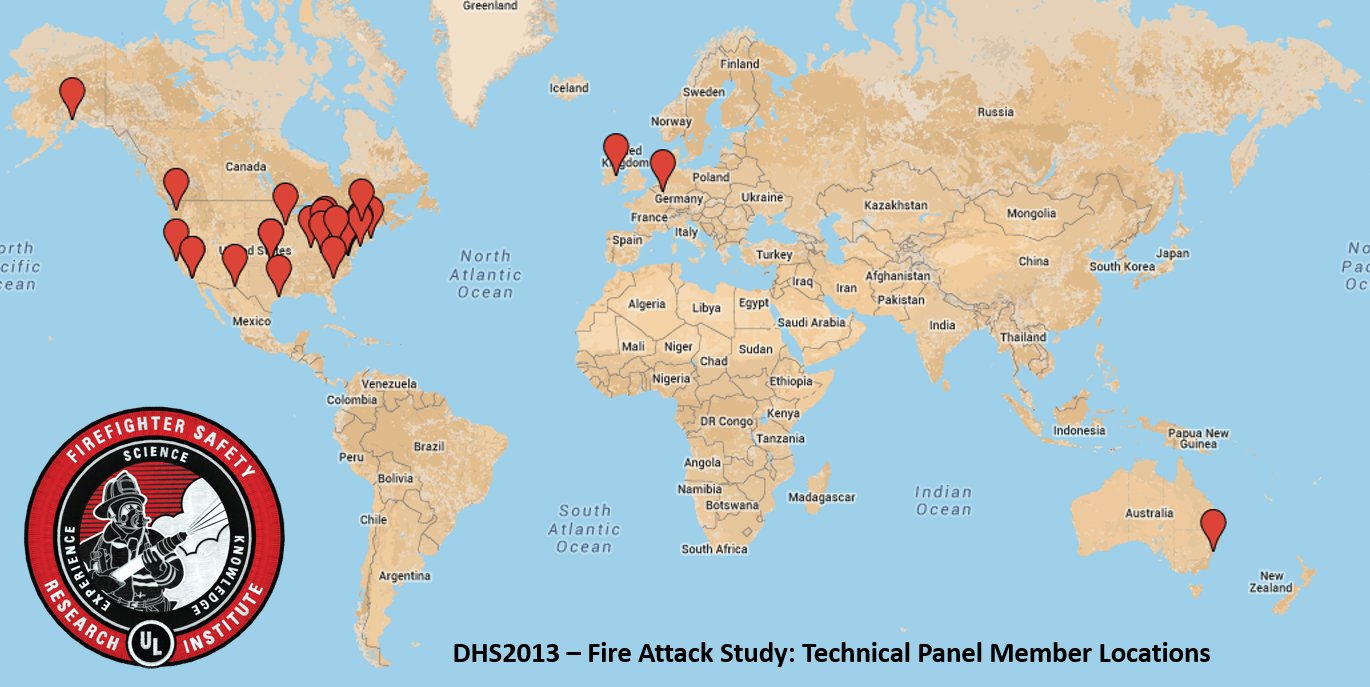
\includegraphics[width = 5in]{Figures/General/Technical_Panel_Logos.png} 
% 	\caption{Fire Attack Technical Panel Member Locations}
% 	\label{fig:PanelLocatoins}
% \end{figure} 

% \clearpage

% The individuals below provided direction for the project, assisting in planing the experiments, witnessing the testing, and developing tactical considerations. Their tireless support and effort make this project relevant to the fire service across the world. 

% \renewcommand{\arraystretch}{1.5}

% \begin{table}[H]
% 	\centering
% 	\caption*{Fire Service Technical Panel}
% 	\begin{tabular}{ll}
% 		\toprule[1.5pt]
% 		Name & Fire Department \\ 
% 		\midrule
% 		Steve Brisebois  & Montreal Fire Department \\ 
% 		Matt Carrigan    & Montgomery County Fire and Rescue Service \\ 
% 		Tony Carroll     & Washington DC Fire Department \\ 
% 		Albert Castillo  & Houston Fire Department \\ 
% 		Chad Christensen & Los Angeles County Fire Department \\ 
% 		John Chubb       & Dublin Fire Brigade \\ 		 		  
% 		Danny Doyle      & Pittsburgh Fire Department \\ 
% 		Aaron Fields     & Seattle Fire Department \\ 
% 		Jason Floyd      & Las Cruces Fire Department \\ 
% 		John Gallagher   & Boston Fire Department \\ 
% 		Chad Green       & Anchorage Fire Department \\ 
% 		Kelly Hanink     & Eden Prairie Fire Department \\ 
% 		Samuel Hittle    & Wichita Fire Department \\ 
% 		Jacob Hoffman    & Toledo Fire/Rescue Department \\ 
% 		Josh Hummel      & Howard County Department of Fire and Rescue Services \\ 
% 		Jerry Knapp      & West Haverstraw (NY) Fire Department \\ 
% 		Dennis Legear    & Oakland Fire Department \\ 
% 		Hans Neiling     & Zuid Limburg Fire \\ 
% 		Nick Martin      & Columbia Fire Department \\ 
% 		Ray McCormack    & Fire Department of New York \\ 
% 		John McDonough   & New South Wales Fire Department \\ 
% 		Jordan Mohr      & Sedgwick County Fire District 1 \\ 
% 		Steve Pegram     & Goshen Township Fire and EMS \\ 
% 		\bottomrule[1.25pt]
% 	\end{tabular}
% \end{table}

% \clearpage

% \chapter{Previous Literature}

% At the start of the study, a literature review was performed to identify and analyze the following:

% \begin{itemize}
% 	\item Previous research in the field of air entrainment, water distribution, and fire suppression
% 	\item Previous research into victim burns and survivability in fires
% 	\item Both past and current fire suppression tactics 
% 	\item Knowledge gaps in fire suppression operations (choice of tactics, myths, traditions, etc.) 
% \end{itemize}

% The following section outlines some of the material as it relates to the fire attack study. The literature review encompassed past research work, various articles in fire service publications, fire service training manuals, fire department standard operating procedures, as well as line of duty injury/death reports to highlight some of the critical areas of information which drove the project at hand.

% \section{Literature Overview}

% Hose, nozzles and water have been used by the fire service for hundreds of years. Despite their frequent use, there has been little scientific research conducted on the effective use of these tools for fire suppression. It is common in the fire service to find discussions about which nozzle is better or which flow rate is required for what sized fire but this is based on experience and usually not science. 

% In 1950 Chief Lloyd Layman presented a paper titled “Little Drops of Water” at the Fire Department Instructors Conference. He introduced what he called indirect method of attack to suppress interior building fires by using the heat absorbing properties of expanding and condensing steam, produced in great quantities by fog streams. The conclusions were based on Coast Guard experiments that Layman was in charge of conducting at the Coast Guard Firefighting School at Fort McHenry in Baltimore, MD. Layman continued his experiments after he returned to his position as fire chief in Parkersburg, WV where he applied his tactic in building fires.  This research had a very large impact on the fire service and their suppression techniques to this day. 

% Throughout the 1950’s a National Committee began conducting experiments to collect data on the growth and behavior of interior fires and how to most effectively suppress them. Keith Royer and Bill Nelson were members of this committee, and as the heads of the firemanship training program at the Iowa State University’s Engineering Extension, they collected and analyzed data from hundreds of experimental fires. Through this research the fire service was taught about fire behavior and how to suppress fire with a combination fire attack. They examined the amount of heat generated by common fuels, the heat absorbing capacity of water, the impact of compartment volume during suppression and they developed the Iowa formula. The Iowa formula or critical rate of flow formula is still used today and it determines the amount of water needed to control a fire in the largest open space within a structure by dividing the cubic foot volume of the space by 100.

% While the physics of fire development has not changed over time, the fire environment for specifically the single family home has evolved. Several factors including home size, geometry, contents and construction materials have changed significantly over the past 50 or more years. Each of these factors has impacted firefighter and occupant safety. Faster fire propagation, shorter times to flashover, rapid changes in fire dynamics and shorter escape times all impact fire service suppression techniques and effectiveness. Many of the variables in Royer and Nelson’s analysis have changed and more research is needed to see how suppression techniques used in the 1950’s with 1950’s fuel loads and firefighting tools translates to today’s firefighter safety and effectiveness.

% Beginning in 1994, the Naval Research Laboratory carried out a series of full-scale fire experiments to compare straight stream attack versus fog pattern attack. These experiments were conducted on the Navy ship ex-USS Shadwell with a fire volume of approximately 110~m$^3$. In these experiments one 60 degree fog pattern was applied at a 45 degree angle into the smoke layer. They examined cooling effects, steam generation and thermal layer disruption. Their experiments examined shielded and non-shielded fires and concluded that using fog to cool the upper layer was more effective and safer than straight stream attack when the fire could not be attacked directly and the firefighters heart rates and body temperatures were lower utilizing the fog attack.

% In 1998 NIST conducted a series of experiments to demonstrate the suppression effectiveness of water-based firefighting agents. This was a step toward creating test procedures to determine suppression effectiveness to develop a standardized test method for evaluating the fire fighting effectiveness of water and other agents. This study provides preliminary data upon which firefighting effectiveness test may be developed by it suggests additional research on application technique, tests reflective of the complexities found in firefighting and experiments involving structural-fire suppression.  

% In 2002, The National Research Council of Canada conducted a literature search on 3D water fog techniques for firefighting. It discusses the impact of water fog characteristics associated with properties of the nozzle (e,g,, droplet size, momentum, flow rate, spray angle and pattern) and discharge techniques (e.g., discharge angle, and discharge duration related to the burts) on performance of the 3D water fog technique are discussed. This technique is to supplement a direct attack by controlling the environment the firefighters are in until they are in a position to apply water directly to the fire. Opponents of flowing water into smoke have concerns that include: (i) effectiveness of controlling the fire, compared to traditional straight stream attack; (ii) possible disruption of the thermal balance; (iii) possible generation of a large amount of hot steam that produces burn injuries to firefighters; and (iv) the performance of this technique is complex and requires extensive training. Advocates of this technique have attempted to respond to these concerns but very limited experimental studies have been undertaken do to complexity of the problems. Application techniques and fire conditions on the the performance of fog technique is not well studied and therefore there are little guidelines and adoption will be greatly limited.

% Several theoretical studies had been conducted that examine droplet size and their ability to suppress fire gases. For example, when droplet diameter is reduced from 1000 nanometers to 100 nanometers the total surface area increases 10 times from 6 m2 to 60 m2 for 1 liter of water. Since these smaller droplets evaporate sooner, others have examined the lifetime of the droplet to determine how far it can travel based on temperature of the surrounding gases and droplet size. Further complicating this theory is that droplets all have an impact on each other as they turn to steam. Residence time can be further reduced compared to an individual droplet, because leading droplets impart forward momentum to the surrounding gas, reducing the air drag on the following droplets and resulting in better penetration. In 2010, the University of Maryland examined spray characteristics from fire hose nozzles. They examined the breakup of a smooth bore nozzle utilizing techniques such as shadowgraphy and a patternator and concluded that more research was needed to fully understand the water spray from fire hose nozzles.  

% In 2000, Lund University examined the demand for extinguishing media in manual firefighting. They examined critical flow rates required to suppress fires by reviewing available literature and conducted a series of experiments that examined suppression of wood pallets at a fire training academy. They examined the five ways that water can be applied during fire extiguishment, on hot gases, on flames, on burning fuel, on fuel that is not yet burning and on hot surfaces. They highlight that what is most effective against the fire is not necessarily best for the firefighters since there are other constraints during firefighting operations such as limited air supply and multiple priorities. The optimum flow rate corresponds to an optimum control time, a control time that gives the lowest total demand for resources. Most of the current data for optimum water flow rate include experiments utilizing wood cribs or pallets, but not todays synthetic fuel loads in actual structures.  These studies also did not investigate the effect of flow paths or the impact of steam generation on firefighters or victims.

% In 2003, a fire service group at the Rockland County (NY) Fire Training Center conducted a series of tests in their concrete training building. They measured the amount of air moved by solid bore and combination nozzles using common fire ground methods. They concluded that air volumes moved by smooth bore nozzles and combination nozzles in the straight stream setting are very similar if not the same, and that combination nozzles in the fog pattern move significant amounts of air which can over pressurize the fire area and send steam over the attack crew even with a ventilation opening opposite the attack crew. These tests were performed either with no fire or with a training fire but which are very different than actual fire conditions. Their tests do provide a good range of airflows that can be expected in our experiments. The authors state, “Our nozzle testing program was not as controlled and as precise as we would have liked.” They also did not have measurement devices that were able to accurately measure air flows from a fog pattern.  

% The Firefighting Technology Group at NIST has a current project that is examining hose streams. This project examines a variety of fire fighting hose stream characteristics related to flow, distribution and thermal impact from both solid and fog stream nozzles. A series of real scale, laboratory based experiments have been started to look specifically at the water discharge and distribution characteristics, the impact of hose streams on a hot gas layer in a compartment, the impact of hose streams on gas flows through multi-compartment structures, and the suppression effectiveness on burning piles of wooden pallets. The proposed project will build on their results by utilizing real-scale structures with common residential fuels and making additional measurements to better characterize the impact of flow path, nozzle technique and steam generation on fire dynamics, firefighter exposure and occupant survivability.

% \section{Fire Service Publications}

% [MIKE]

% \section{Fire Service Training Manuals}

% [MIKE]

% \section{Firefighter Line of Duty Deaths}

% [MIKE]

% \section{Research Work}

% [MIKE]

% \clearpage

\clearpage

\chapter{Experimental Configuration}

\section{Test Fixtures}

The ranch fire experiments were conducted in two identical structures that were constructed in UL's Large Fire Test Facility in Northbrook, IL. The 1620 $ft^2$ houses were designed by a residential  architectural company to be typical of a single family home constructed in the late-20th century in the United States. The floor plan included 4 bedrooms, a bathroom, a living area, kitchen, and dining room. Three of the bedrooms were left open during the fire experiments, while one bedroom (Bedroom 3) was left closed, to examine the impact of a closed door on fire behavior. The interior of the house had 8' ceilings, and the rooms were separated from each other with walls and doorways. The floor plan of the houses used for these experiments can be seen in Figure \ref{figure:ranchexp1_floorplan}.

\begin{figure}[H]
\centering
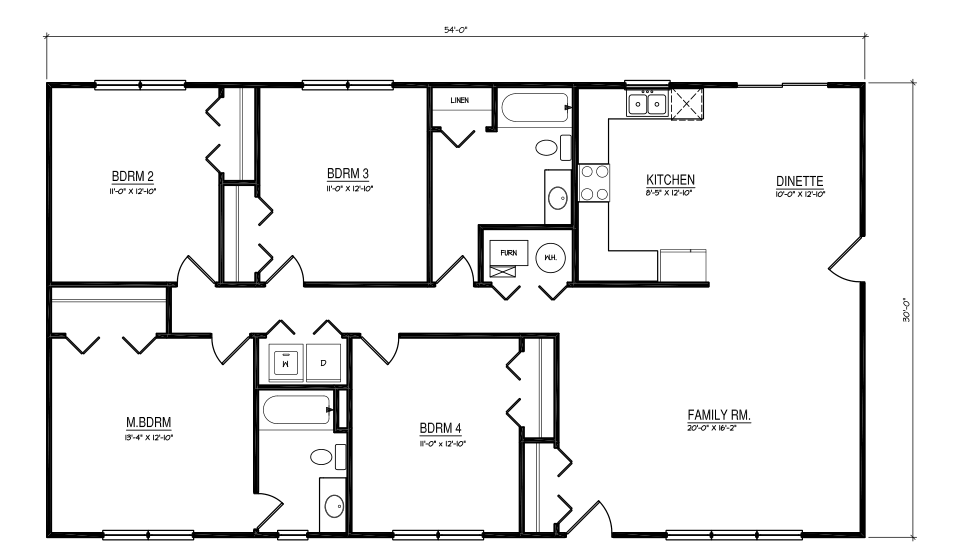
\includegraphics[width=\textwidth]{0_Images/Ranch_Pictures/Ranch_Floor_Plan.png}
\caption{Ranch Floor Plan}
\label{figure:ranchexp1_floorplan}
\end{figure}

Since the ranch fire experiments were intended to examine room and contents fires, and not structure fires, the walls of the fire room (Bedroom 1) and hallway were lined with two layers of gypsum board: a surface layer of 1/2'' board and a base layer of 5/8'' board. The remaining interior surfaces in the structure consisted of 1/2'' drywall. The exterior walls were covered with cement board to limit exterior fire spread. In Experiments 1 and 2, the floor close to the fire room and in the kitchen area was composed of cement board. The rest of the house was carpeted. For Experiment 3, the kitchen floor was composed of cement board, while the rest of the house was carpeted. The layout for Experiments 1 and 2 can be seen in Figure \ref{figure:ranchexp2_floorplan}, and the layout for Experiment 3 can be seen in Figure \ref{figure:ranchexp3_floorplan}.

\begin{figure}[H]
\centering
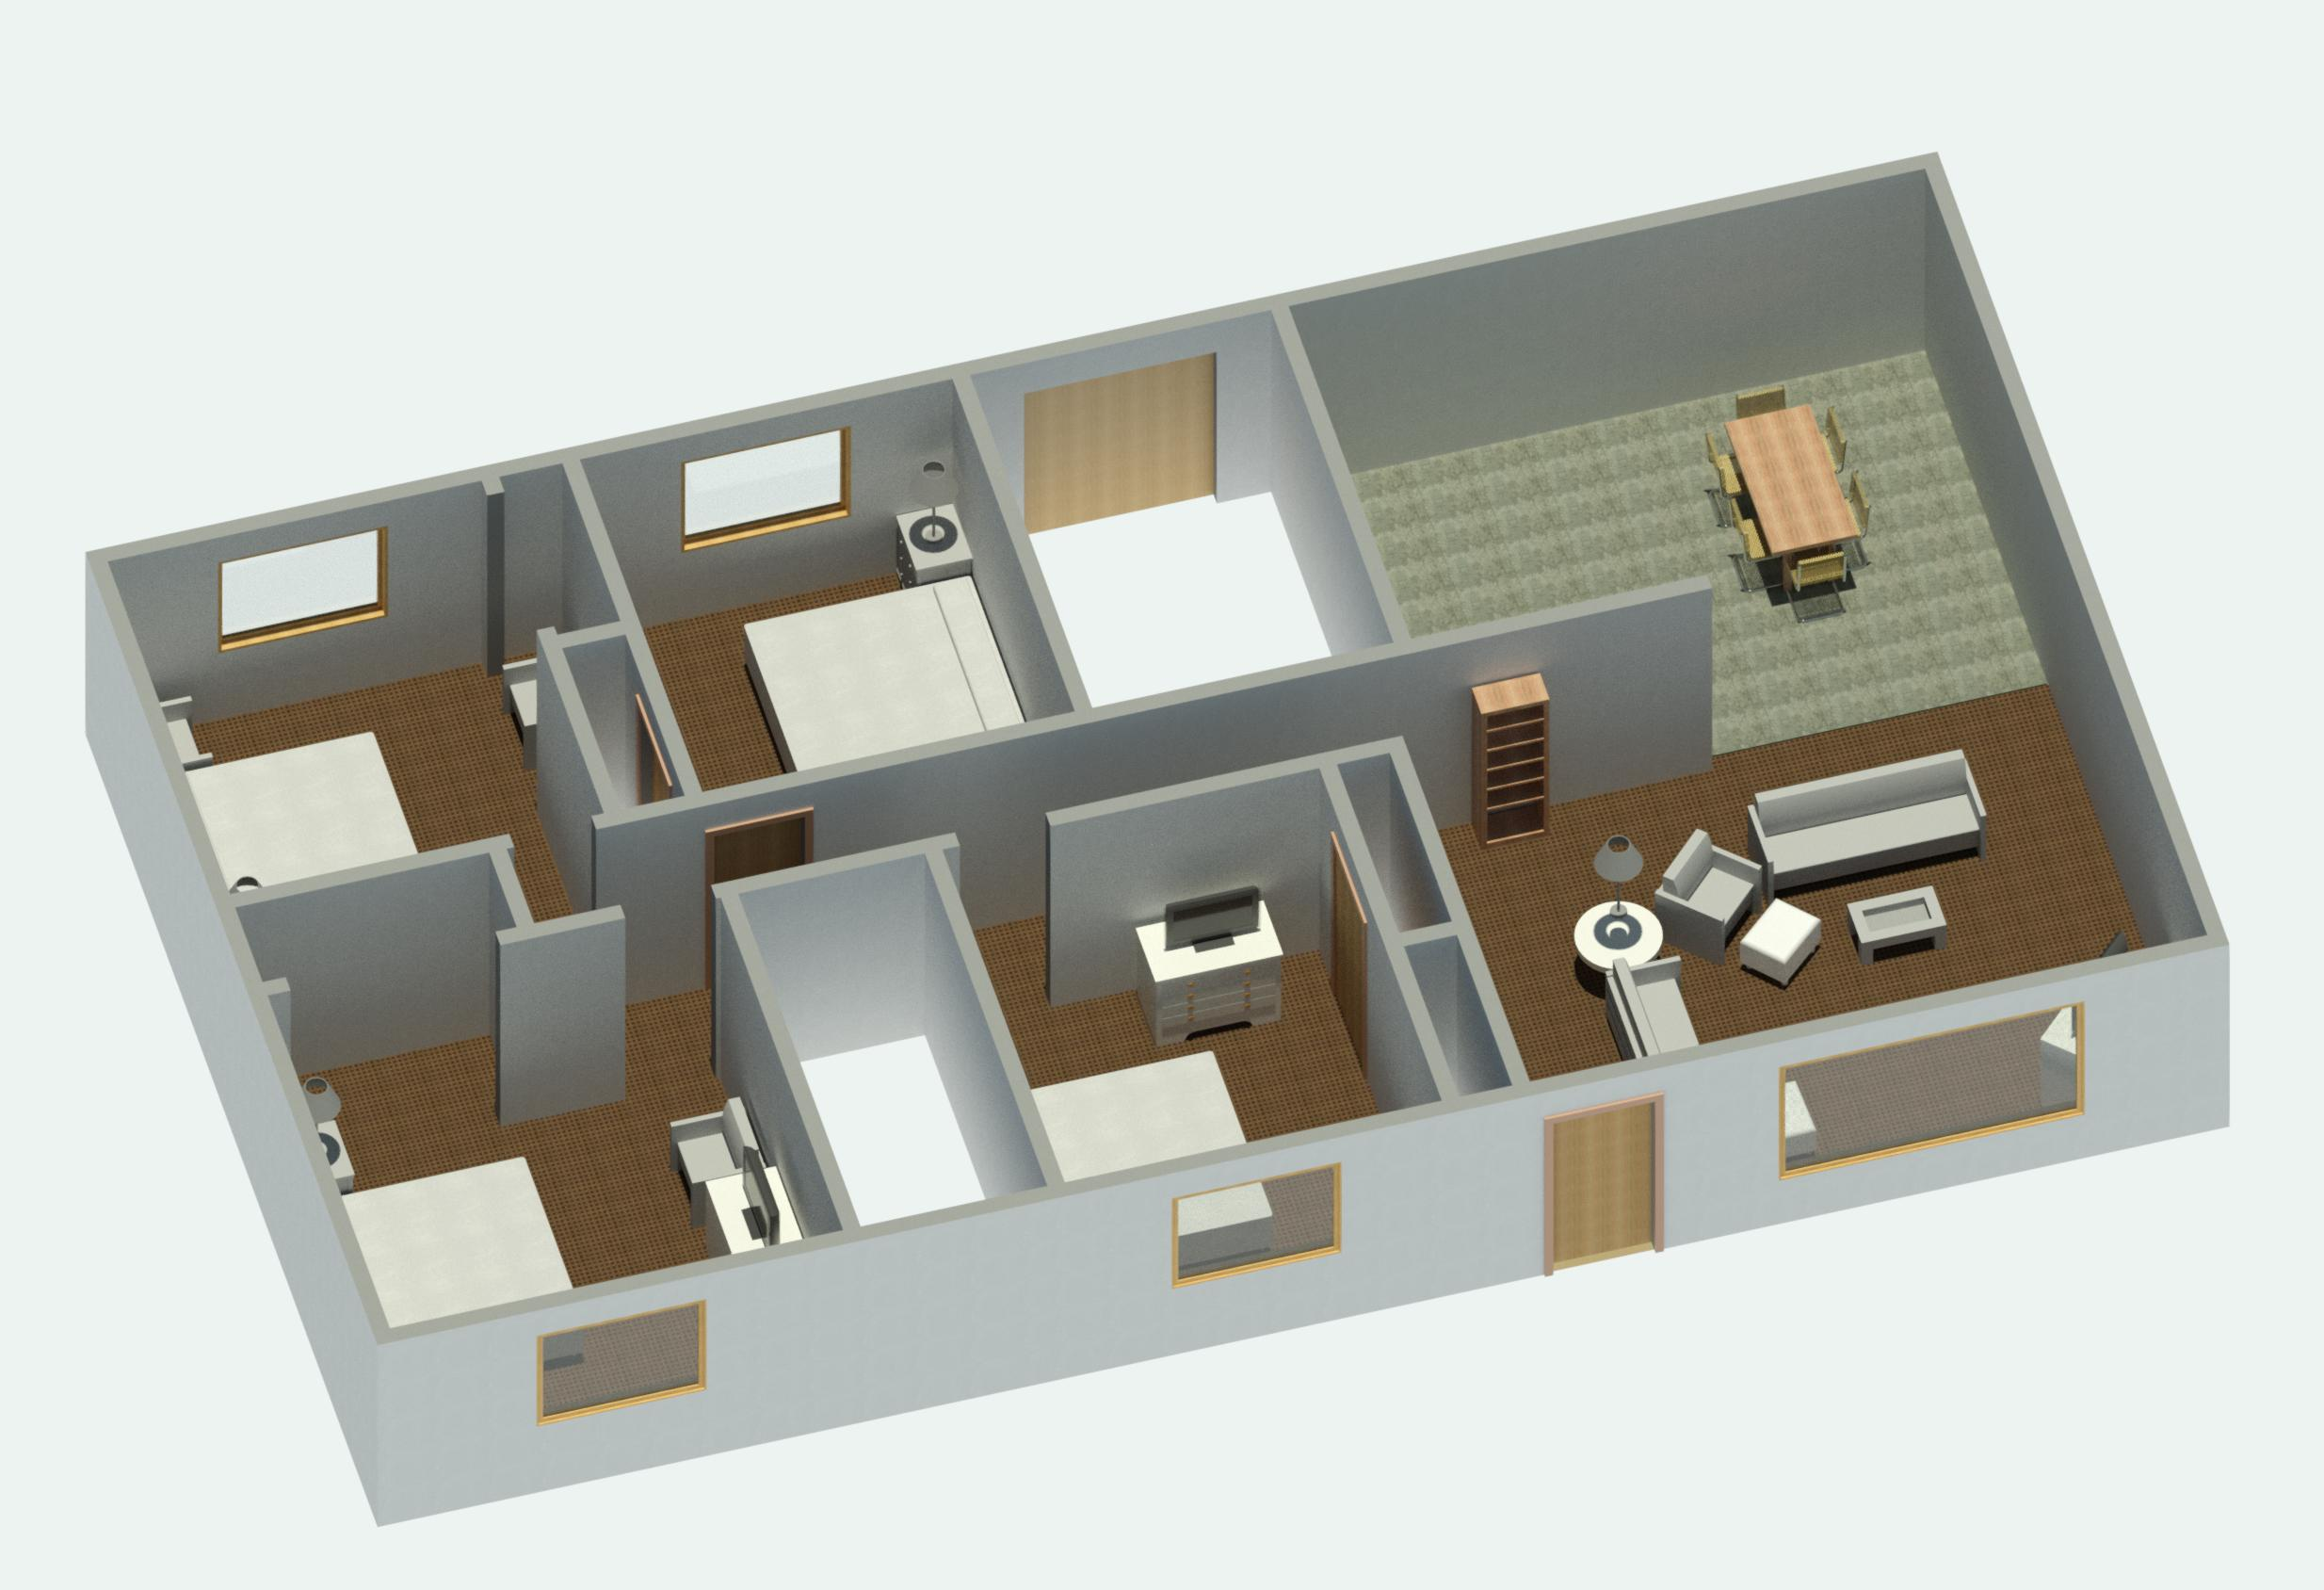
\includegraphics[width=.75\textwidth]{0_Images/Ranch_Pictures/Report_ISO_Furniture.jpg}
\caption{Furnished Experiment Layout}
\label{figure:ranchexp3_floorplan}
\end{figure}

\section{Fuel Loads}
 In Experiment 1, the only fuel in the fire room was three wooden pallets and 1/3 bale of straw,  arranged in a ``teepee'' formation, as shown in Figure \ref{figure:Exp1_fuel}. The middle of the teepee was filled with 13 lbs. of straw.  Experiment 2 had an identical configuration of pallets and straw, but also included six  48'' x 96'' x 7/16'  sheets of OSB. Three of these sheets lined the wall behind the fire set, and three lined the ceiling above it, as shown in \ref{figure:Exp2_fuel}. In both of the training fuel experiments, the fire was ignited remotely with an electric match in the center of the teepee. In Experiment 3, the fire room was furnished to simulate a typical bedroom in a residential home. The fuel load consisted of a king-sized bed, dresser, TV, nightstand, pillows, 4'' foam mattress topper, 3 stuffed chairs (1 Yellow/Green Chair, 1 Red Lined Chair, and 1 Red Swirl Chair), curtains, carpet, and carpet padding.  The orientation of the fuel can be seen in Figure \ref{figure:Exp3_fuel}. The fire was ignited remotely  with an electric match in the seat cushion of the stuffed armchair at the side of the bed.

\begin{figure}[H]
\centering
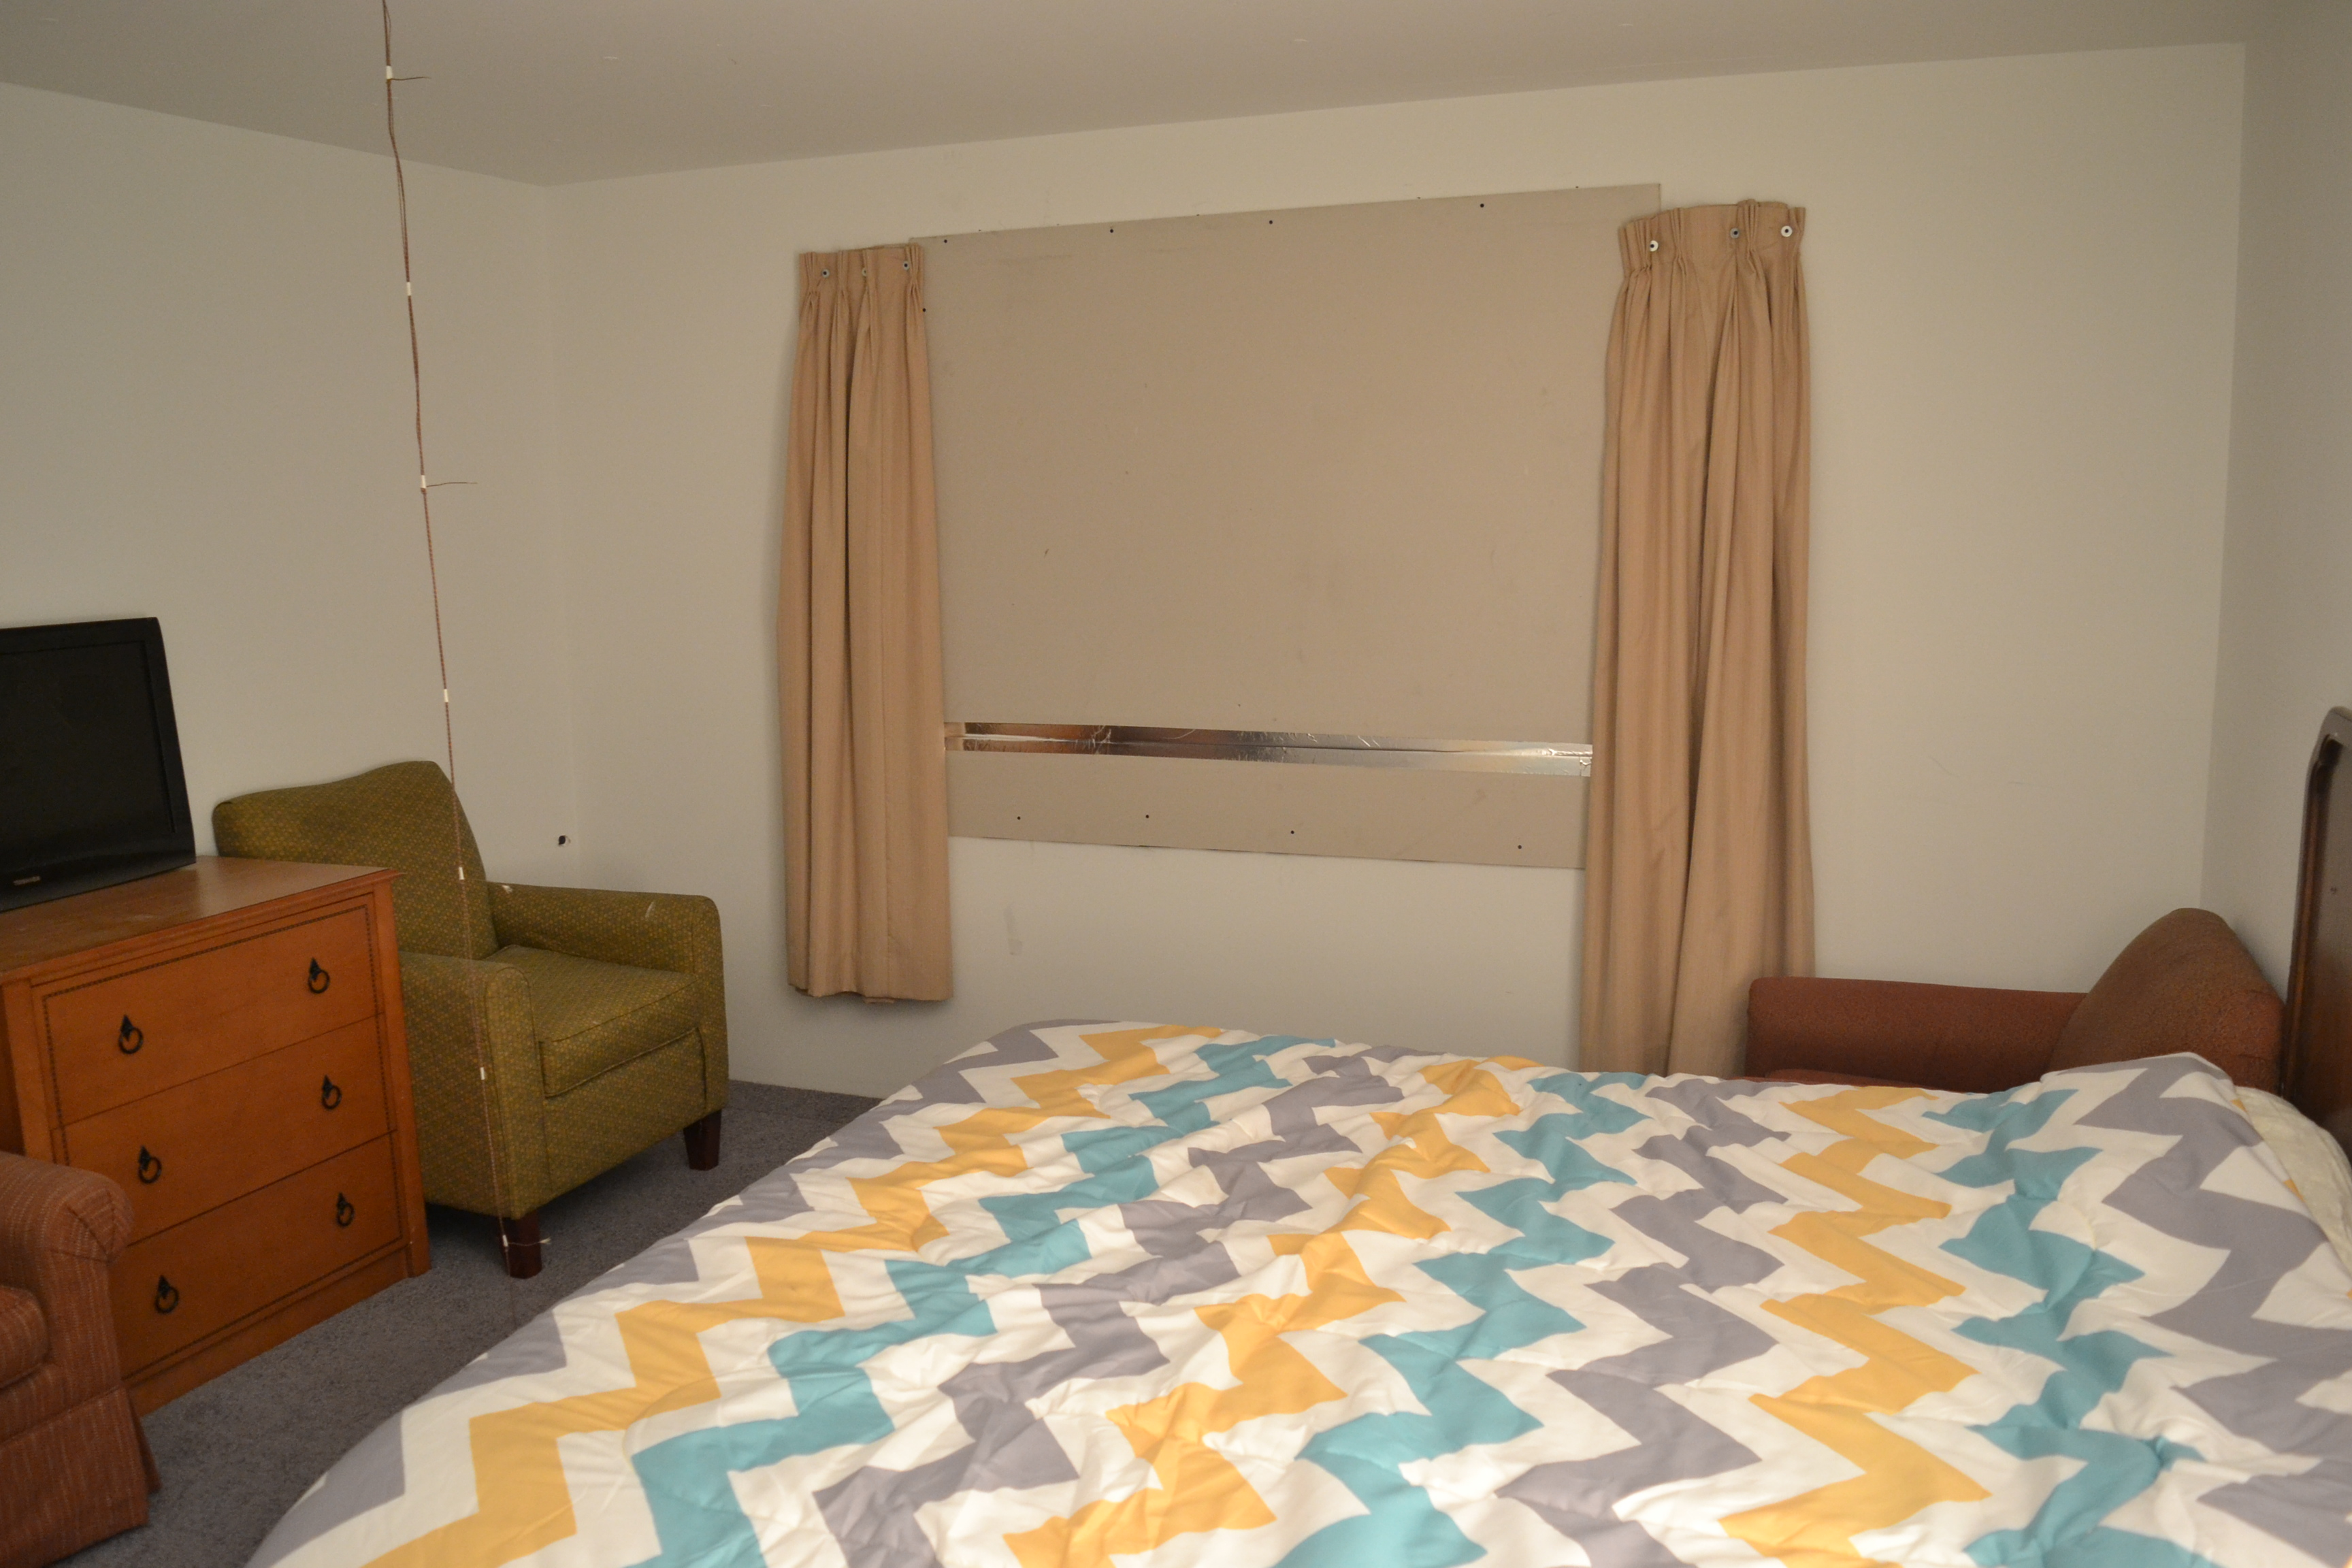
\includegraphics[width=.75\textwidth]{0_Images/Ranch_Pictures/Exp_3_Fuel.jpg}
\caption{Experiment 3 Fuel Orientation}
\label{figure:Exp3_fuel}
\end{figure}

The furniture configuration in areas of the house remote from the fire room was identical for all three experiments. Since the furnishings in these areas of the house were remote from the fire, it was assumed that they did not contribute in any significant way to fire growth.  Bedroom 2 contained 2 stuffed chairs (1 Striped chair and 1 Red Diamond chair), a king-sized bed, dresser, nightstand, pillows, 4'' foam mattress topper, curtains, carpet, and carpet padding. Bedrooms 3 and 4 contained 1 stuffed chair (Yellow/Green Chair), a king-sized bed, dresser, nightstand, pillows, 4'' foam mattress topper, curtains, carpet, and carpet padding. The kitchen contained a kitchen table and 6 chairs. The living room contained a bookshelf with shelves line with a 5" foam mattress topper, 2 sofas, 1 stuffed chair (Yellow/Green chair) 2 ottomans, a coffee table, end table, lamp, TV, TV stand, large curtains, carpet, and carpet padding. The weights and dimensions for each elements of the fuel load are listed in Table \ref{table:fuel_weights}.

\begin{table}
\scalebox{0.7}{
\centering
\begin{tabular}{|l|c|c|c|c|l|}
\hline
Item & Length (in) & Width (in) & Height (in) & Weight (lbs.) & Material \\ \hline \hline
King Mattress & 79 & 71 & 10 & 76 & 52\% Polyurethane Foam, 30\% \\ &&&&& Blended Cotton Batting  \& 18\% Polyester\\ &&&&& Fiber Batting \\ \hline
King Boxspring & 78 & 35 & 7 & 46 & 59\% Fiber Pad, 41\% Blended Cotton \\ &&&&& Batting \& Wood Frame \\ \hline
King Headboard & 78 & 24 & 1 & 54 & Medium Density Fiberboard \\ \hline
Pillow & 23.5 & 17 & 4 & 1.5 & Filling - All Polyester, Cover - 100\% Cotton \\ \hline
Comforter & 104 & 92 & 1 & 4.6 & Cover - 100\% Polyester, Fill - 100\% Polyester \\ \hline
Mattress Topper 4 in & 78 & 75 & 3.875 & 16.0  & Viscoelastic Polyurethane Foam Pad 100\% \\ \hline
Mattress Topper 5 in & 77.5 & 76.25 & 4.625 & 20.1  & Urethane Foam \\ \hline
Sofa Chair (Red Diamond) & 35 & 35 & 34 & 69 & Polyurethane Foam (Blended Cotton or\\ &&&&& Polyester when used is less than 10\%) \\ \hline
Sofa Chair (Striped) & 33 & 35 & 33.5 & 65 & Polyurethane Foam 75\% Polyester Fiber 25\% \\ \hline
Sofa Chair (Yellow/Green) & 31.25 & 31 & 39 & 54 & Polyester Fiber 75\%, Polyurethane Foam 25\%,\\ &&&&& Pillow - Polyurethane Foam 90\%, Polyester \\ &&&&& Batting 10\% \\ \hline
Sofa Chair (Red Lines) & 34.5 & 34 & 32 & 63 & Urethane Foam 100\% \\ \hline
Sofa Chair (Red Swirl) & 34 & 34 & 32 & 70 & Blended Cotton Felt 100\%, Cushion -\\ &&&&& Polyurethane Foam 100\% \\ \hline
Night Stand & 18 & 27 & 23.375 & 60 & Solid Wood \\ \hline
Table Lamp & Base - 5.75, & Base - 5.25,  & 31.25 & 5.9 & Glass, Metal \& Cloth Shade \\& Shade - 14.375 & Shade - 14.375&&&\\ \hline 
Dresser & 22.125 & 36 & 34.25 & 120 & Wood \& Plywood \\ \hline
Curtain (Large) & 107 & 73 & 0.125 & 13.7 & Flame Retardant \& Synthetic Fibers \\ \hline
Curtain (Small) & 39 & 73 & 0.125 & 4.5 & Flame Retardant \& Synthetic Fibers \\ \hline
Sofa & 35 & 77 & 30.5 & 255 & Polyurethane Foam 50\%, Polyester Fiber 50\%,\\&&&&& \& Wood Frame \\ \hline
Coffee Table (Rectangular) & 30 & 18 & 18.25 & 24.4 & Particleboard \& Wood \\ \hline
End Table (Circular) & 24.25 & 24.25 & 22.125 & 32.1 & Solid Wood \\ \hline
Footstool & 19.75 & 25.5 & 16 & 21.3 & Upholstery \\ \hline
Bookcase & 11.5 & 24.625 & 71.25 & 46 & Particleboard \\ \hline
Kitchen Table (Square) & 26 & 26 & 24.5 & 29.1 & Particleboard \& Wood \\ \hline
Straight Chair (Pink) & 18 & 19 & 33 & 15.2 & Wood \& Upholstery \\ \hline
Straight Chair (Blue) & 19 & 19 & 38.875 & 14.9 & Wood \& Upholstery \\ \hline
\end{tabular}}
\caption{Fuel Load Information}
\label{table:fuel_weights}
\end{table}

\section{Instrumentation}

Measurements of temperature, heat flux, pressure, and gas velocity were taken at various locations. For the ranch experiments, the same instrumentation was used throughout the duration of the study. The following describes the instrumentation used and potential uncertainty.

Heat flux measurements were made using a 2.54~cm nominal diameter water-cooled Schmidt- Boelter heat flux gauge (Figure \ref{fig:HeatFluxGauge}). The gauges measured the combined radiative and convective heat flux. For these experiments, the dominant form of heat flux is radiative due to the distance of the heat flux gauges from the flames. It should be noted that the convective contribution to the heat flux is dependent upon the surface temperature of the heat flux gauge. The manufacturer gives an uncertainty of $\pm$3~\% and results from a study on heat flux calibration found the typical expanded uncertainty to be $\pm$8~\% \cite{HeatFluxRoundRobin}.

\begin{figure} [H]
	\centering
	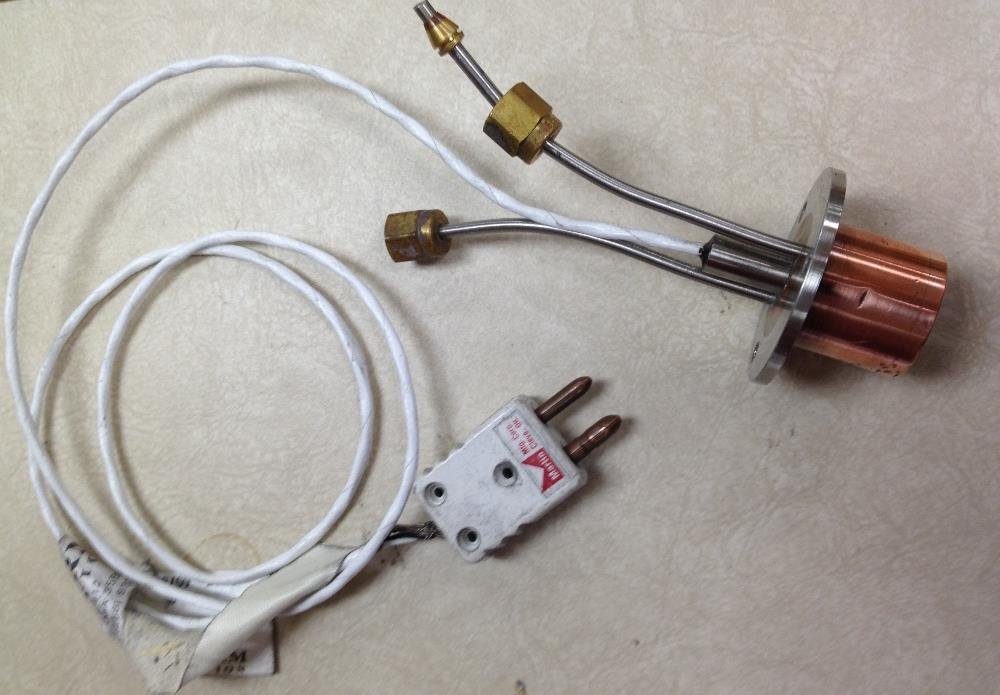
\includegraphics[width = 3.5in]{0_Images/Instrumentation/Heat_Flux_Gauge.jpg}
	\caption{Water Cooled Schmidt-Boelter Heat Flux Gauge}
	\label{fig:HeatFluxGauge}
\end{figure}

Temperatures were recorded using a bare-bead, Chromel-Alumel (Type K) thermocouple with a 0.5 mm nominal diameter (Figure \ref{fig:Thermocouple}). The uncertainty given by the manufacturer for the temperature measurements is $\pm$2.2~$^\circ$C for temperatures below 293~$^\circ$C and $\pm$0.75~\% for higher temperatures \cite{TemperatureHandbook}. The thermocouple readings will be lower than the air temperature when the thermocouple is in the flame region, due to radiative losses to the surrounding cooler environment. When the thermocouples are farther from the flame region, the impact of radiation will result in temperature readings higher than the air temperature. Due to the effect of radiative heat transfer to the thermocouples, the expanded uncertainty is approximately $\pm$15~\%.

\begin{figure} [H]
	\centering
	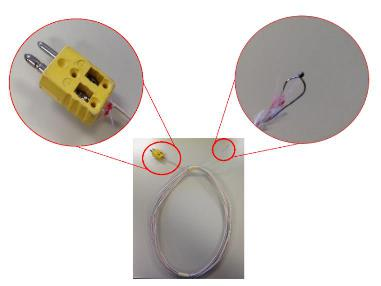
\includegraphics[width = 4in]{0_Images/Instrumentation/Thermocouple.jpg}
	\caption{Chromel-Alumel (Type K) Thermocouple}
	\label{fig:Thermocouple}
\end{figure}

To determine the gas velocity, an array of bi-directional probes was utilized in conjunction with differential pressure transducers and inconel thermocouples. The bi-directional probe was constructed of stainless steel and features a `high' side and a `low' side which travel back to a pressure transducer that evaulates the differential pressure from ambient pressure. The iconel thermocouples were placed in-line wtih the bi-directional probes to ensure that the measurements were recorded at the same location. The iconel thermocouple was a 0.063~in. diameter type KSL iconel 600 sheathed grounded junction with a type K, 24~gauge glass/glass insulation lead. The differential pressure transducer was a Setra Model 264 with a range of ±1.0~in. WC ($\pm$248.8~Pa). The uncertainty given by the manufacturer is 1~\% or 1.2~Pa. The configuration had a velocity range of $\pm$24.2~m/s ($\pm$54~mph). The pressure transducers were configured in groups of 6, contained in a single plastic box with connections for pressure, temperature and power (Figure~\ref{fig:Gas_Velocity_Measurements}a). Five probes were installed in openings where velocity measurements were taken, centered horizontally in the opening (Figure~\ref{fig:Gas_Velocity_Measurements}b). Velocity measurement with this configuration was determined to have an uncertainty of $\pm$18~\% \cite{BDPInPoolFires}.

\begin{figure}[H]
	\centering
	\begin{tabular}{c c}
		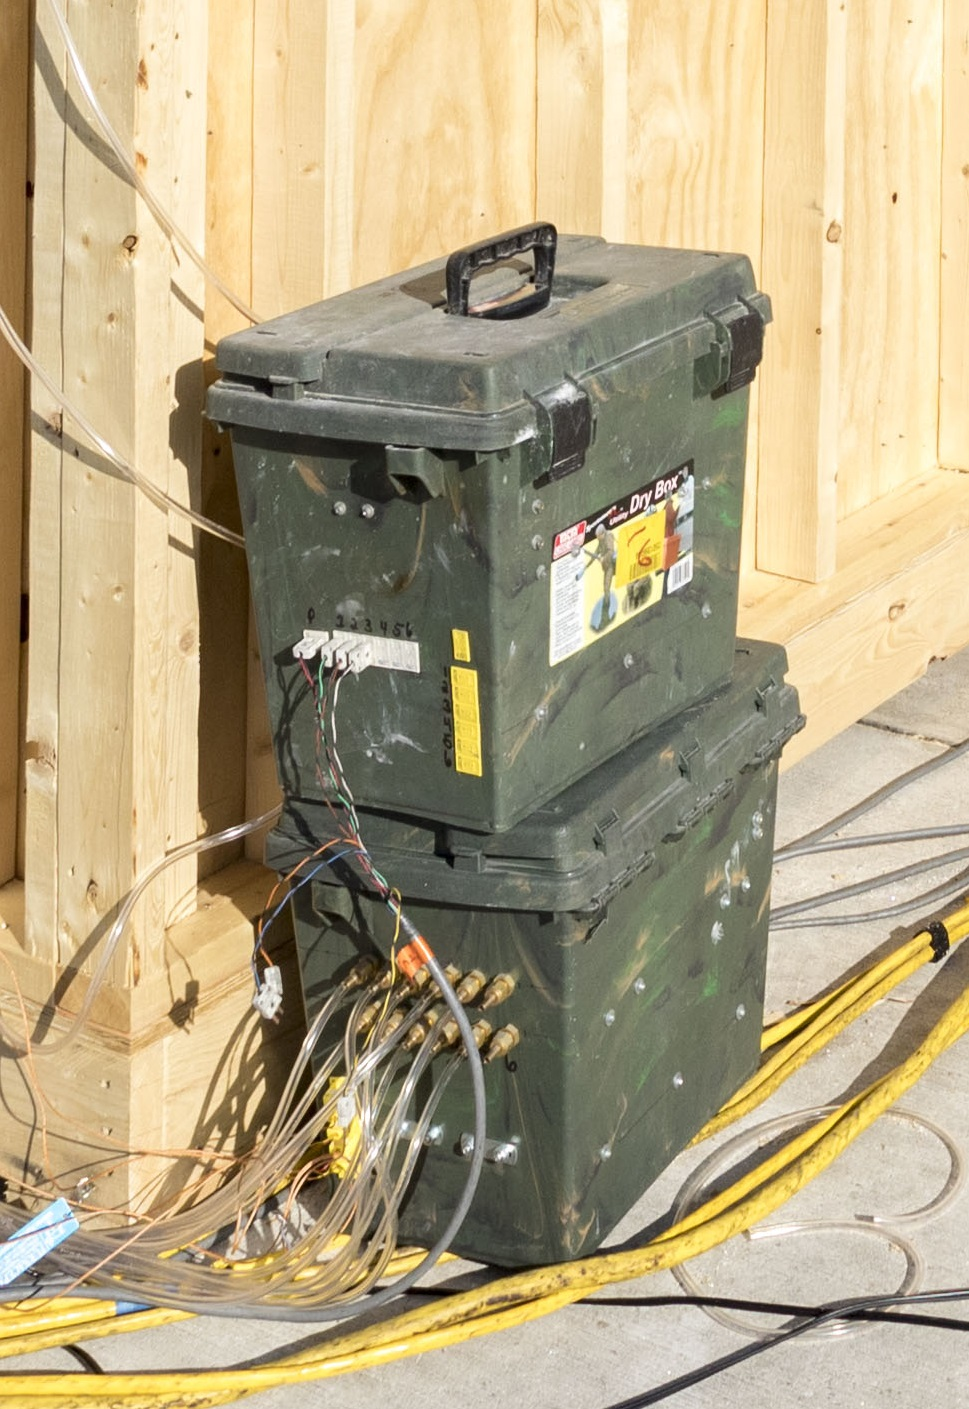
\includegraphics[height = 2.5in]{0_Images/Instrumentation/PressureBox.jpg} &
		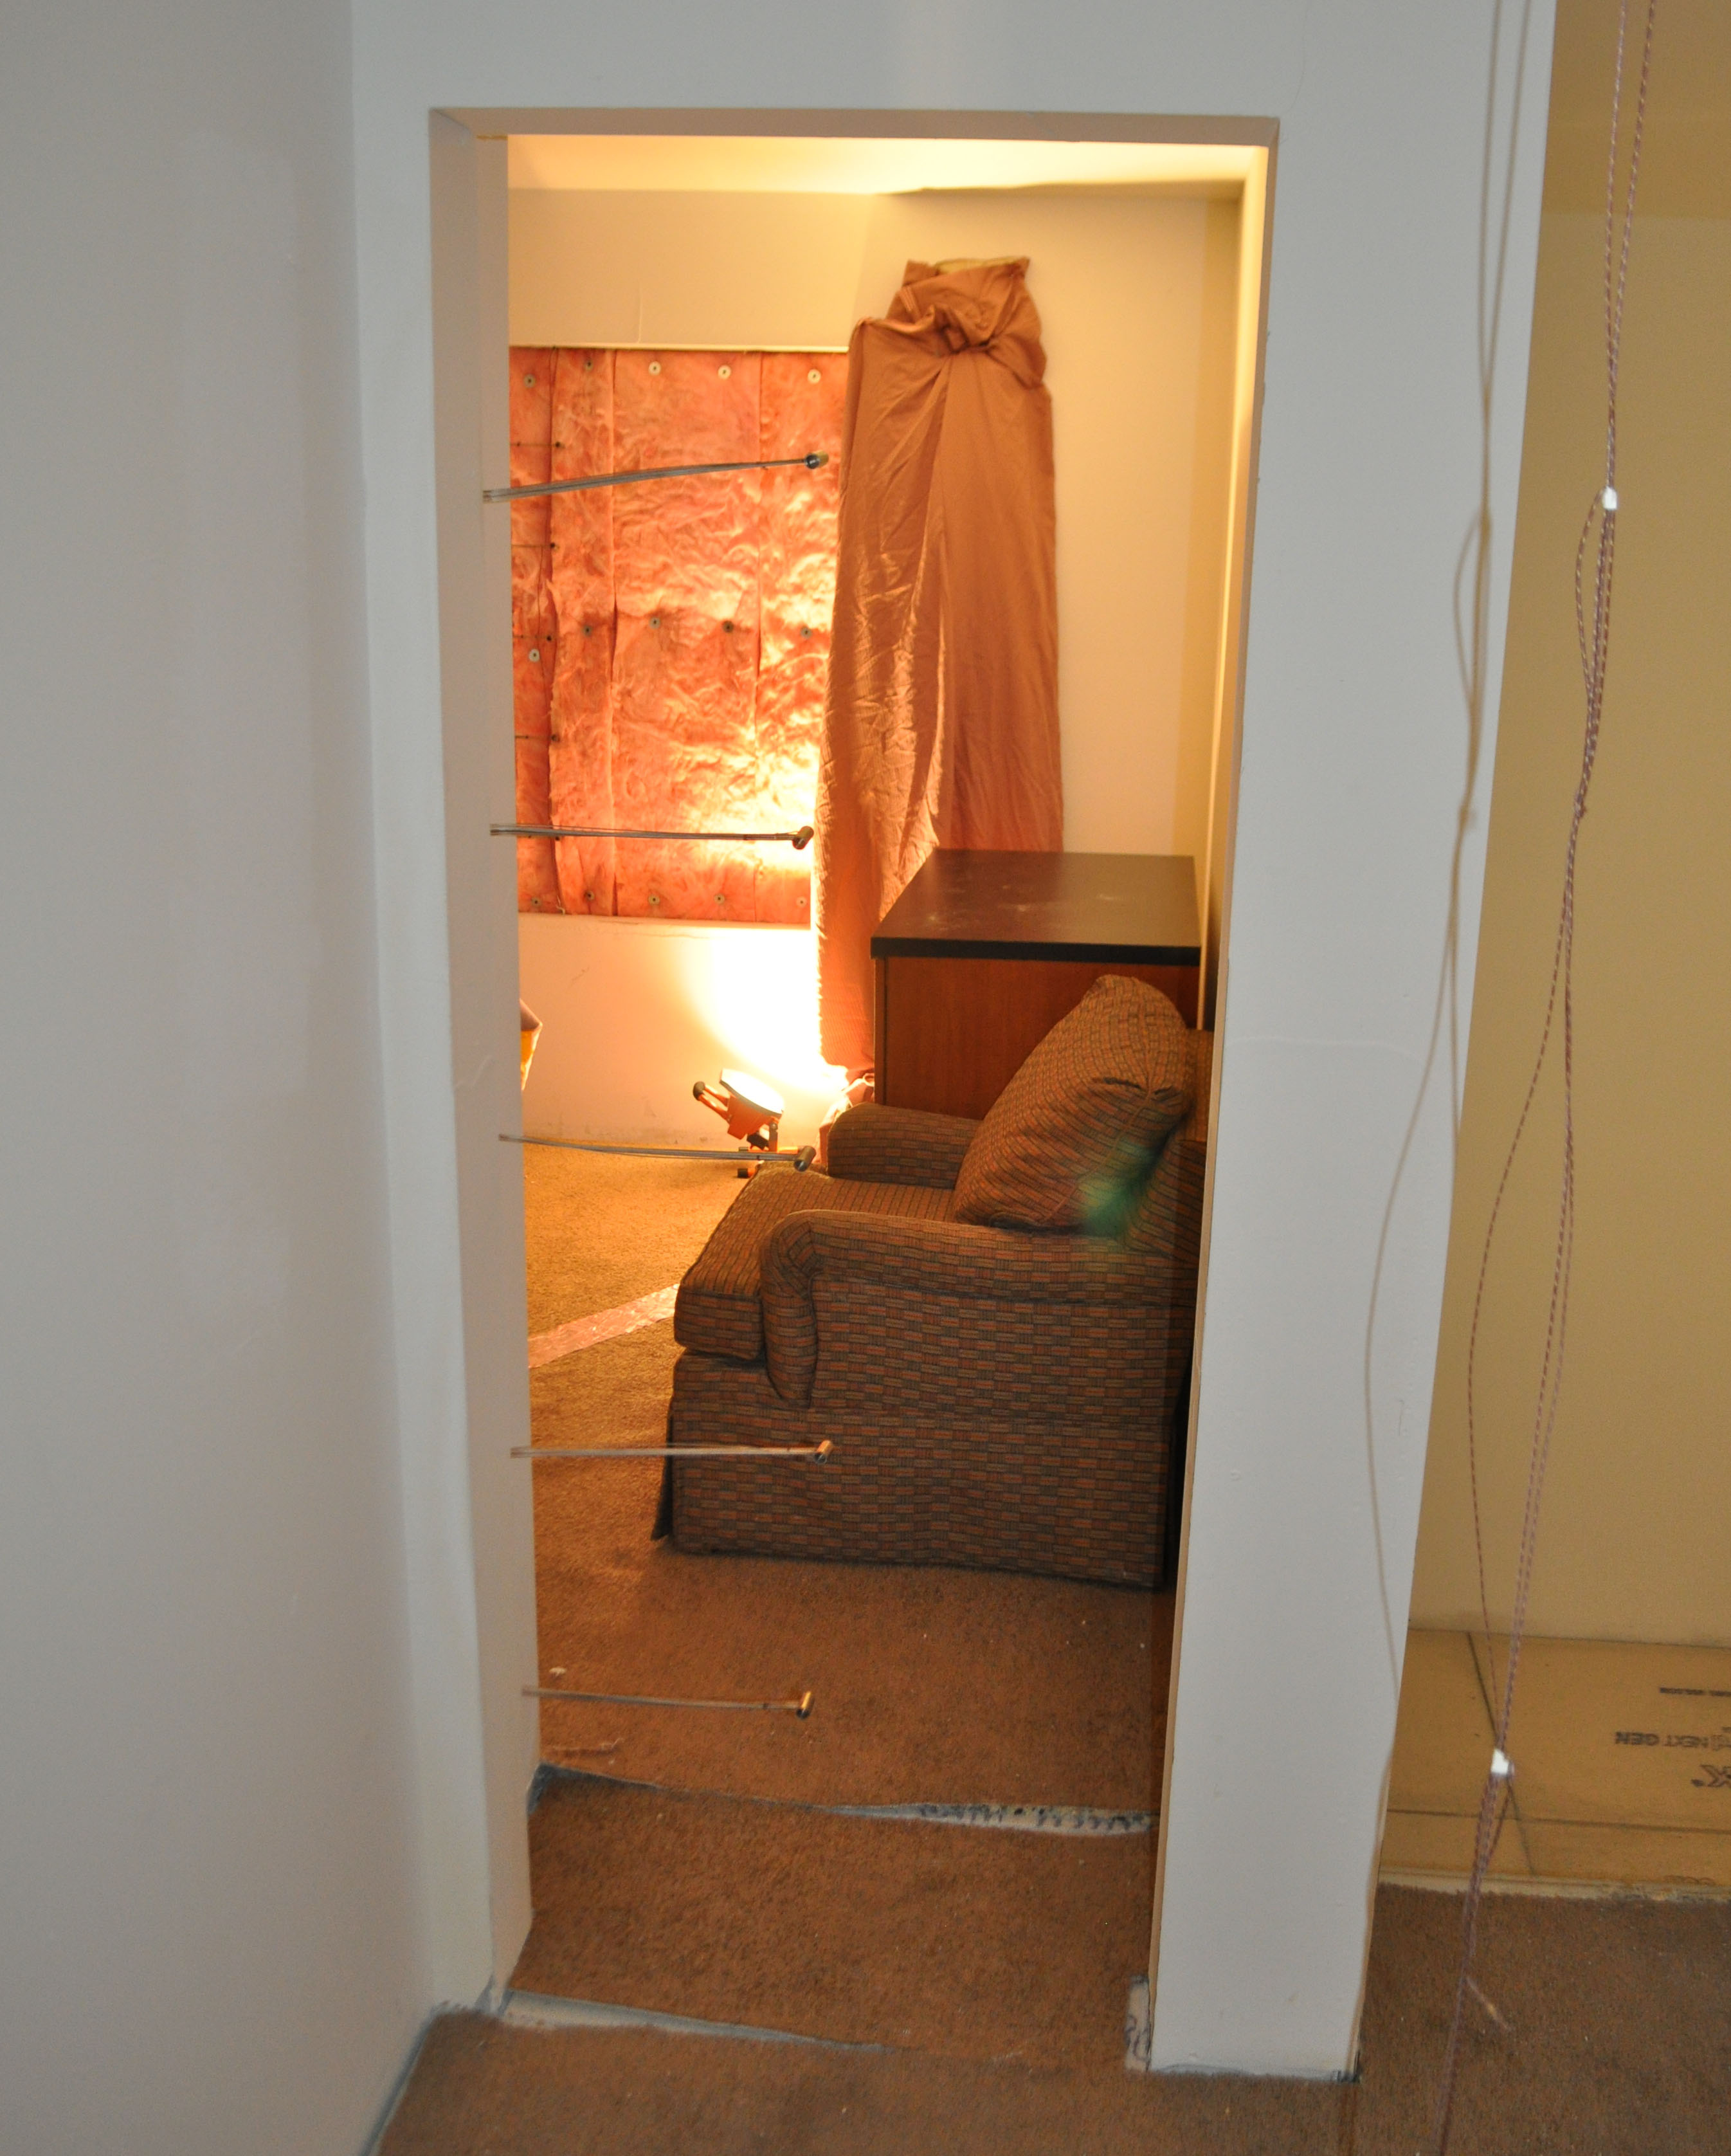
\includegraphics[height = 2.5in]{0_Images/Instrumentation/BDPArray.jpg} \\
	\end{tabular}
	\caption{Bi-Directional Probe}
	\label{fig:BDP}
\end{figure}

Standard video was obtained through the use of BoschVTC-206F03-4 video cameras (Figure~\ref{fig:BullettCam}). Thermal imaging of the front and rear of the structure was taken using ISG Infrasys Elite XR (Figure~\ref{fig:IRCam}). The thermal imaging camera has a fixed emissivity value of 0.9 and was utilized for visual representation of relative conditions, no temperature measurements or analysis were derived using the camera. All cameras were recorded Samsung Model SRD-1680 DN digital video recorder set to 24 frames per second with a quality of ``high''.

\begin{figure}[H]
	\centering
	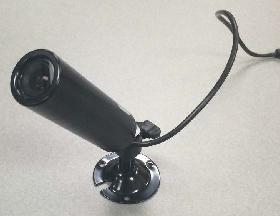
\includegraphics[width = 3in]{0_Images/Instrumentation/BullettCam.jpg}

	\caption{BoschVTC-206F03-4 video camera}
	\label{fig:BullettCam}
\end{figure}

\begin{figure}[H]
	\centering
	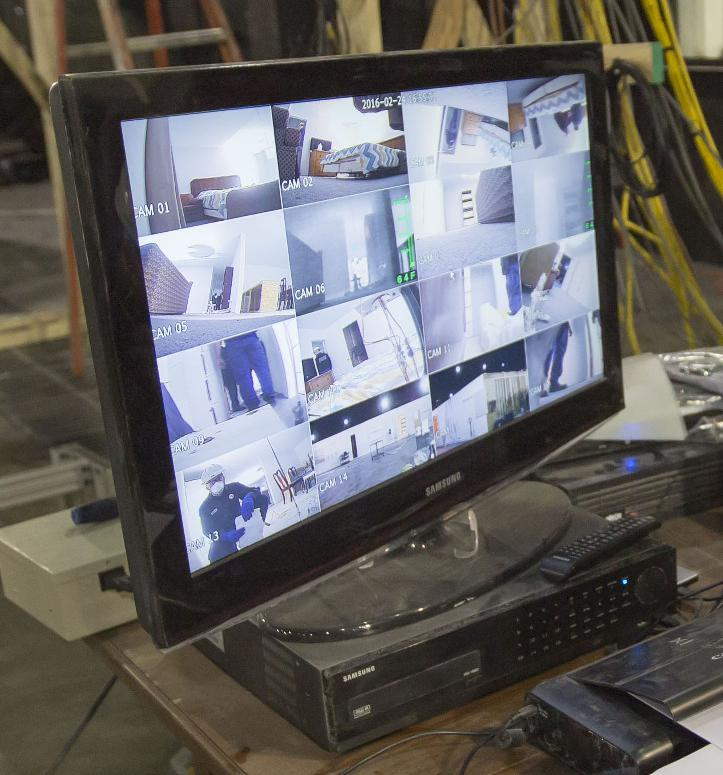
\includegraphics[width = 3in]{0_Images/Instrumentation/DVR.jpg}

	\caption{Samsung Model SRD-1680 DN Digital Video Recorder with Monitor}
	\label{fig:DVR}
\end{figure}

\begin{figure}[H]
	\centering
	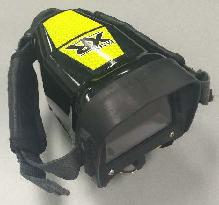
\includegraphics[width = 2.5in]{0_Images/Instrumentation/ISG_IR.jpg}
	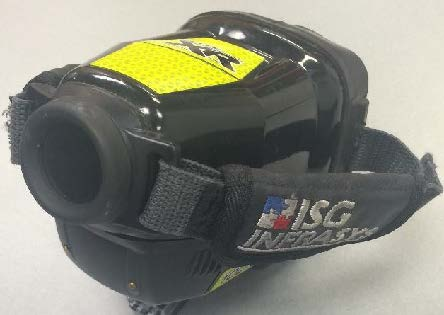
\includegraphics[width = 2.5in]{0_Images/Instrumentation/ISG_IR2.jpg}
	\caption{ISG Elite XR Fire Service Thermal Imaging Camera}
	\label{fig:IRCam}
\end{figure}

Gas samples were analyzed through the use of OxyMat6 and UltraMat23 Siemens gas analyzers. Samples were pulled from the structure through the use of Cole Palmer Model L-79200-30 vacuum/pressure diaphragm pump rated at 0.75~CFM via a stainless steel tube. The sample is filtered through a course filter, Solberg Model 842, 2 micron paper filter before running through a condensing trap to remove moisture. The sample then runs through a drying tube dry fine filter, Perma Pure Model FF-250-SG-2.5G with a 1 micron filter FF-250-E-2.5G before splitting into two branches and entering the UltraMat and OxyMat analyzer. The analyzers are calibrated to measure CO from 0-50000~PPM, CO$_2$ from 0-20~\% and O$_2$ from 0-25~\%. 

\begin{figure}[H]
	\centering
	\begin{minipage}[b]{0.5\linewidth}
		\centering
		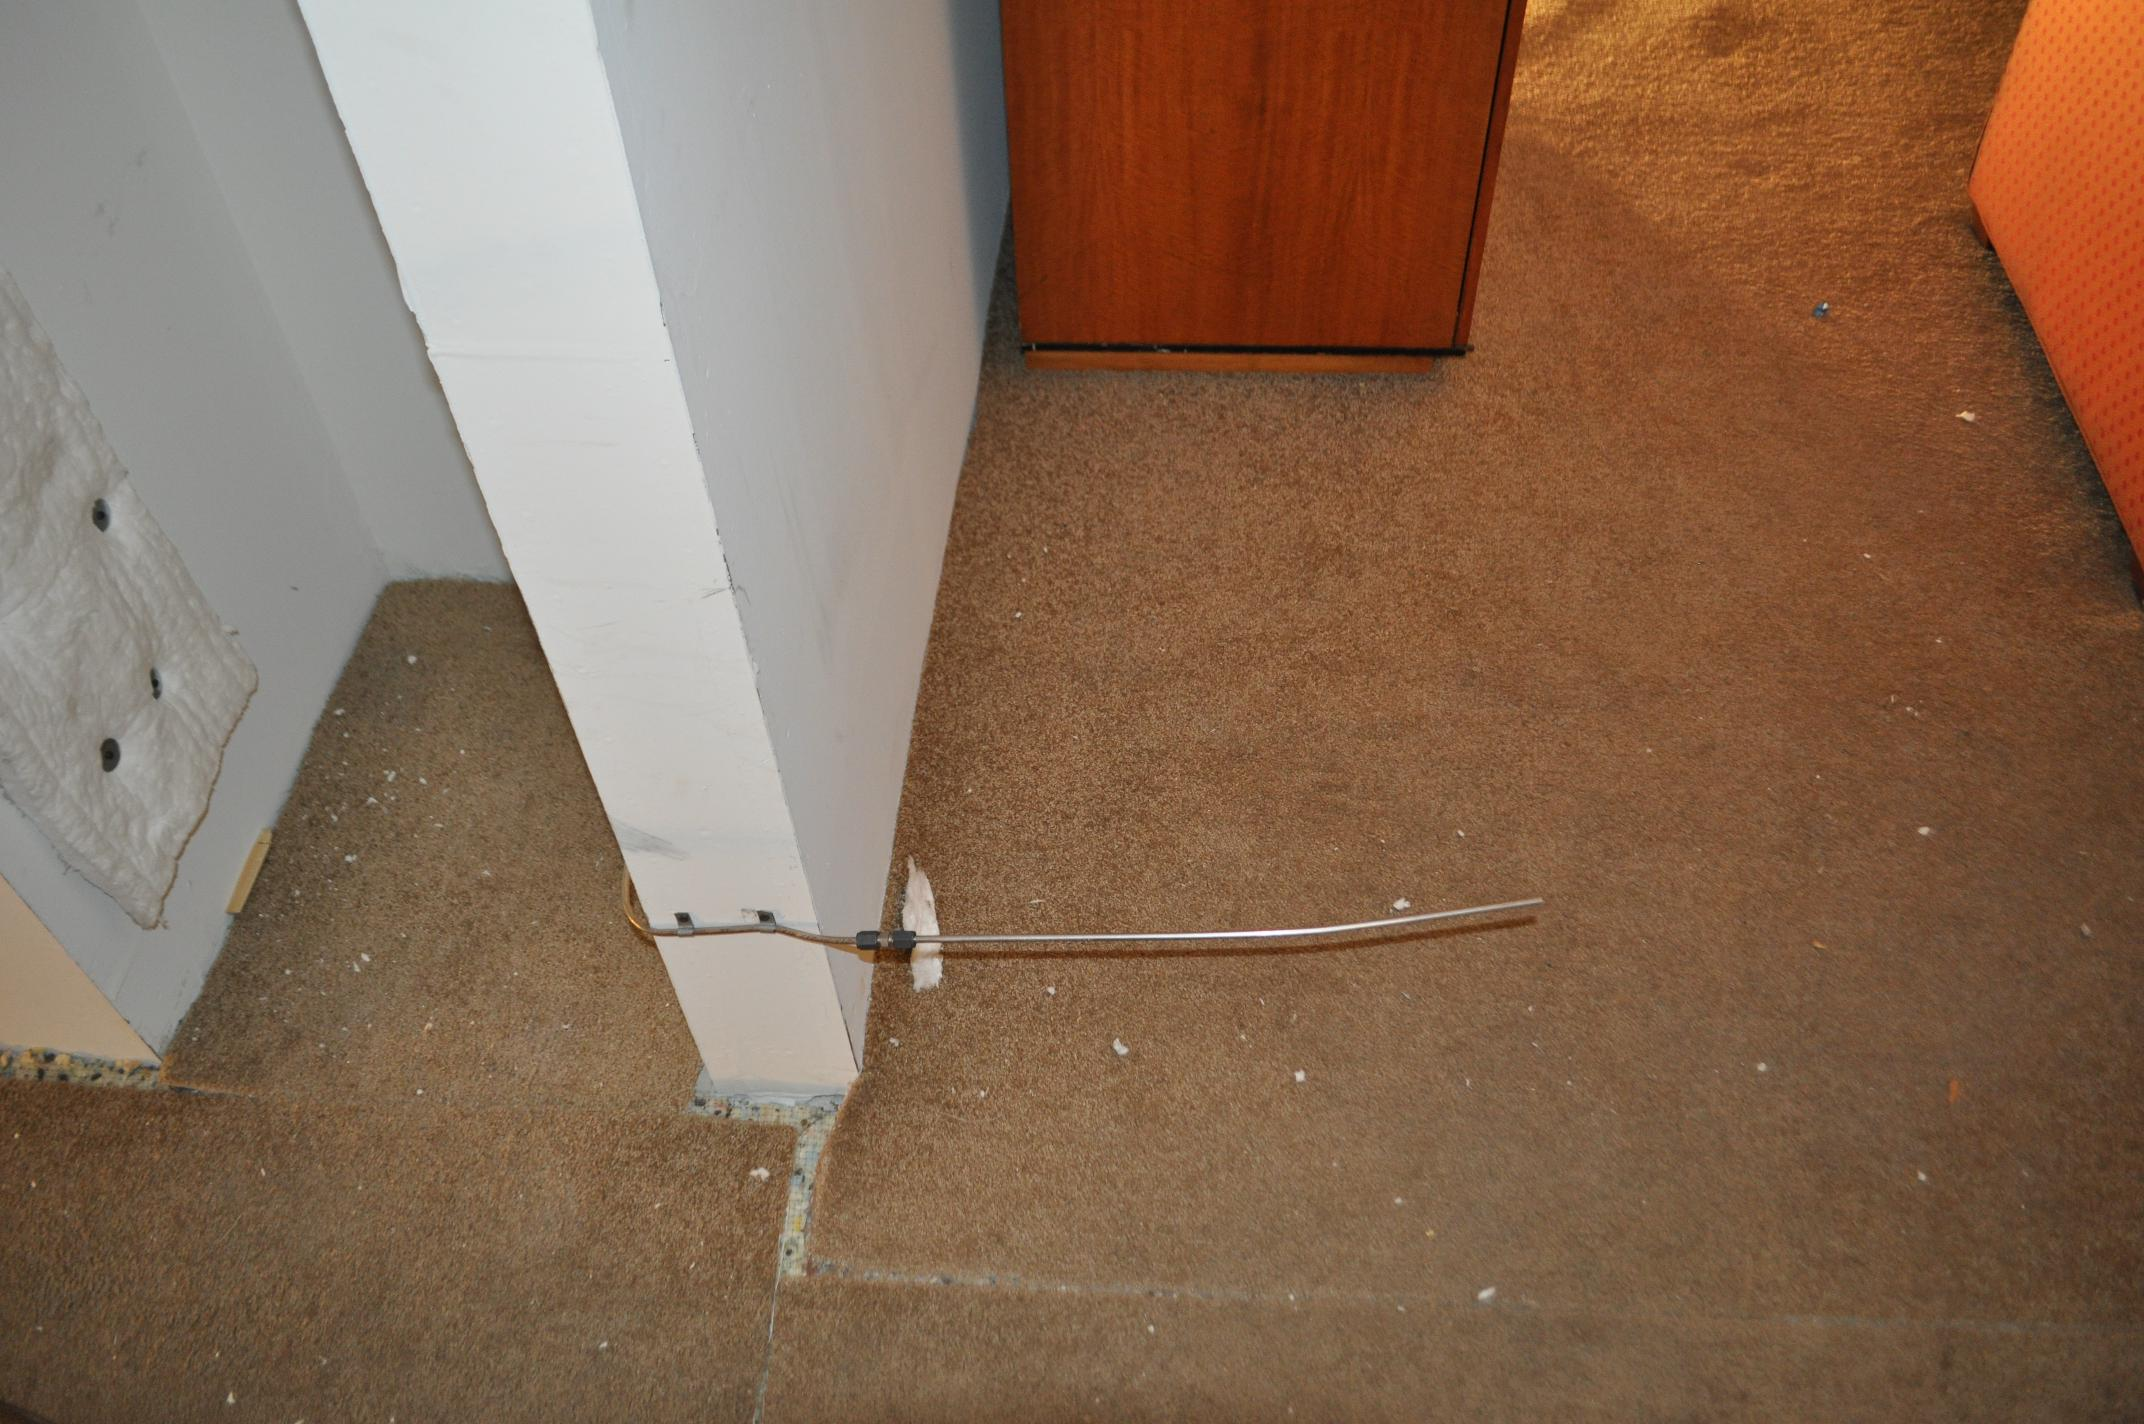
\includegraphics[width = 2in]{0_Images/Instrumentation/Gas_Analyzer/SamplePoint.jpg}
		\subcaption{Gas Sample Point}
	\end{minipage}

	\begin{minipage}[b]{0.5\linewidth}
		\centering
		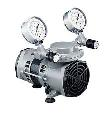
\includegraphics[width = 2in]{0_Images/Instrumentation/Gas_Analyzer/VaccumPump.jpg}
		\subcaption{Vaccum Pump - Cole Palmber L-79200-30}
	\end{minipage}
	
	\begin{minipage}[b]{0.5\linewidth}
		\centering
		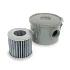
\includegraphics[width = 2in]{0_Images/Instrumentation/Gas_Analyzer/CourseFilter.jpg}
		\subcaption{Course Filter - Solberg 842}
	\end{minipage}
	
	\begin{minipage}[b]{0.5\linewidth}
		\centering
		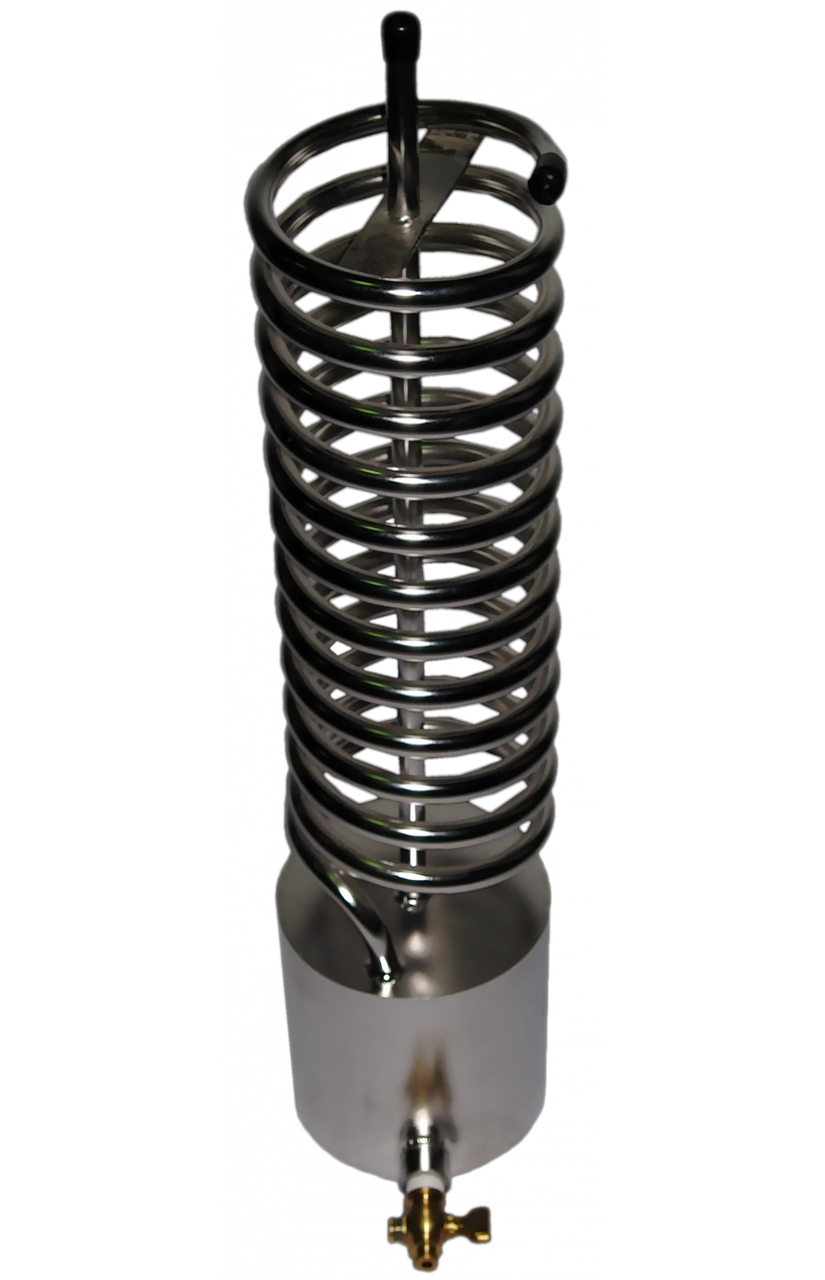
\includegraphics[height = 2in]{0_Images/Instrumentation/Gas_Analyzer/CoilCondenser.png}
		\subcaption{Condensing Tube}
	\end{minipage}
	
	\begin{minipage}[b]{0.5\linewidth}
		\centering
		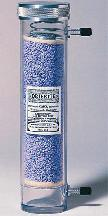
\includegraphics[height = 2in]{0_Images/Instrumentation/Gas_Analyzer/DriRightTube.jpg}	
		\subcaption{Dririte Tube}
	\end{minipage}

	\begin{minipage}[b]{0.5\linewidth}
		\centering
		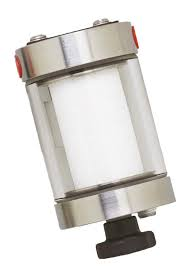
\includegraphics[height = 2in]{0_Images/Instrumentation/Gas_Analyzer/FineFilter.jpg}
		\subcaption{Fine Filter - Perma Pure FF-250-SG-2.5G}
	\end{minipage}

	\begin{minipage}[b]{0.5\linewidth}
	\centering
		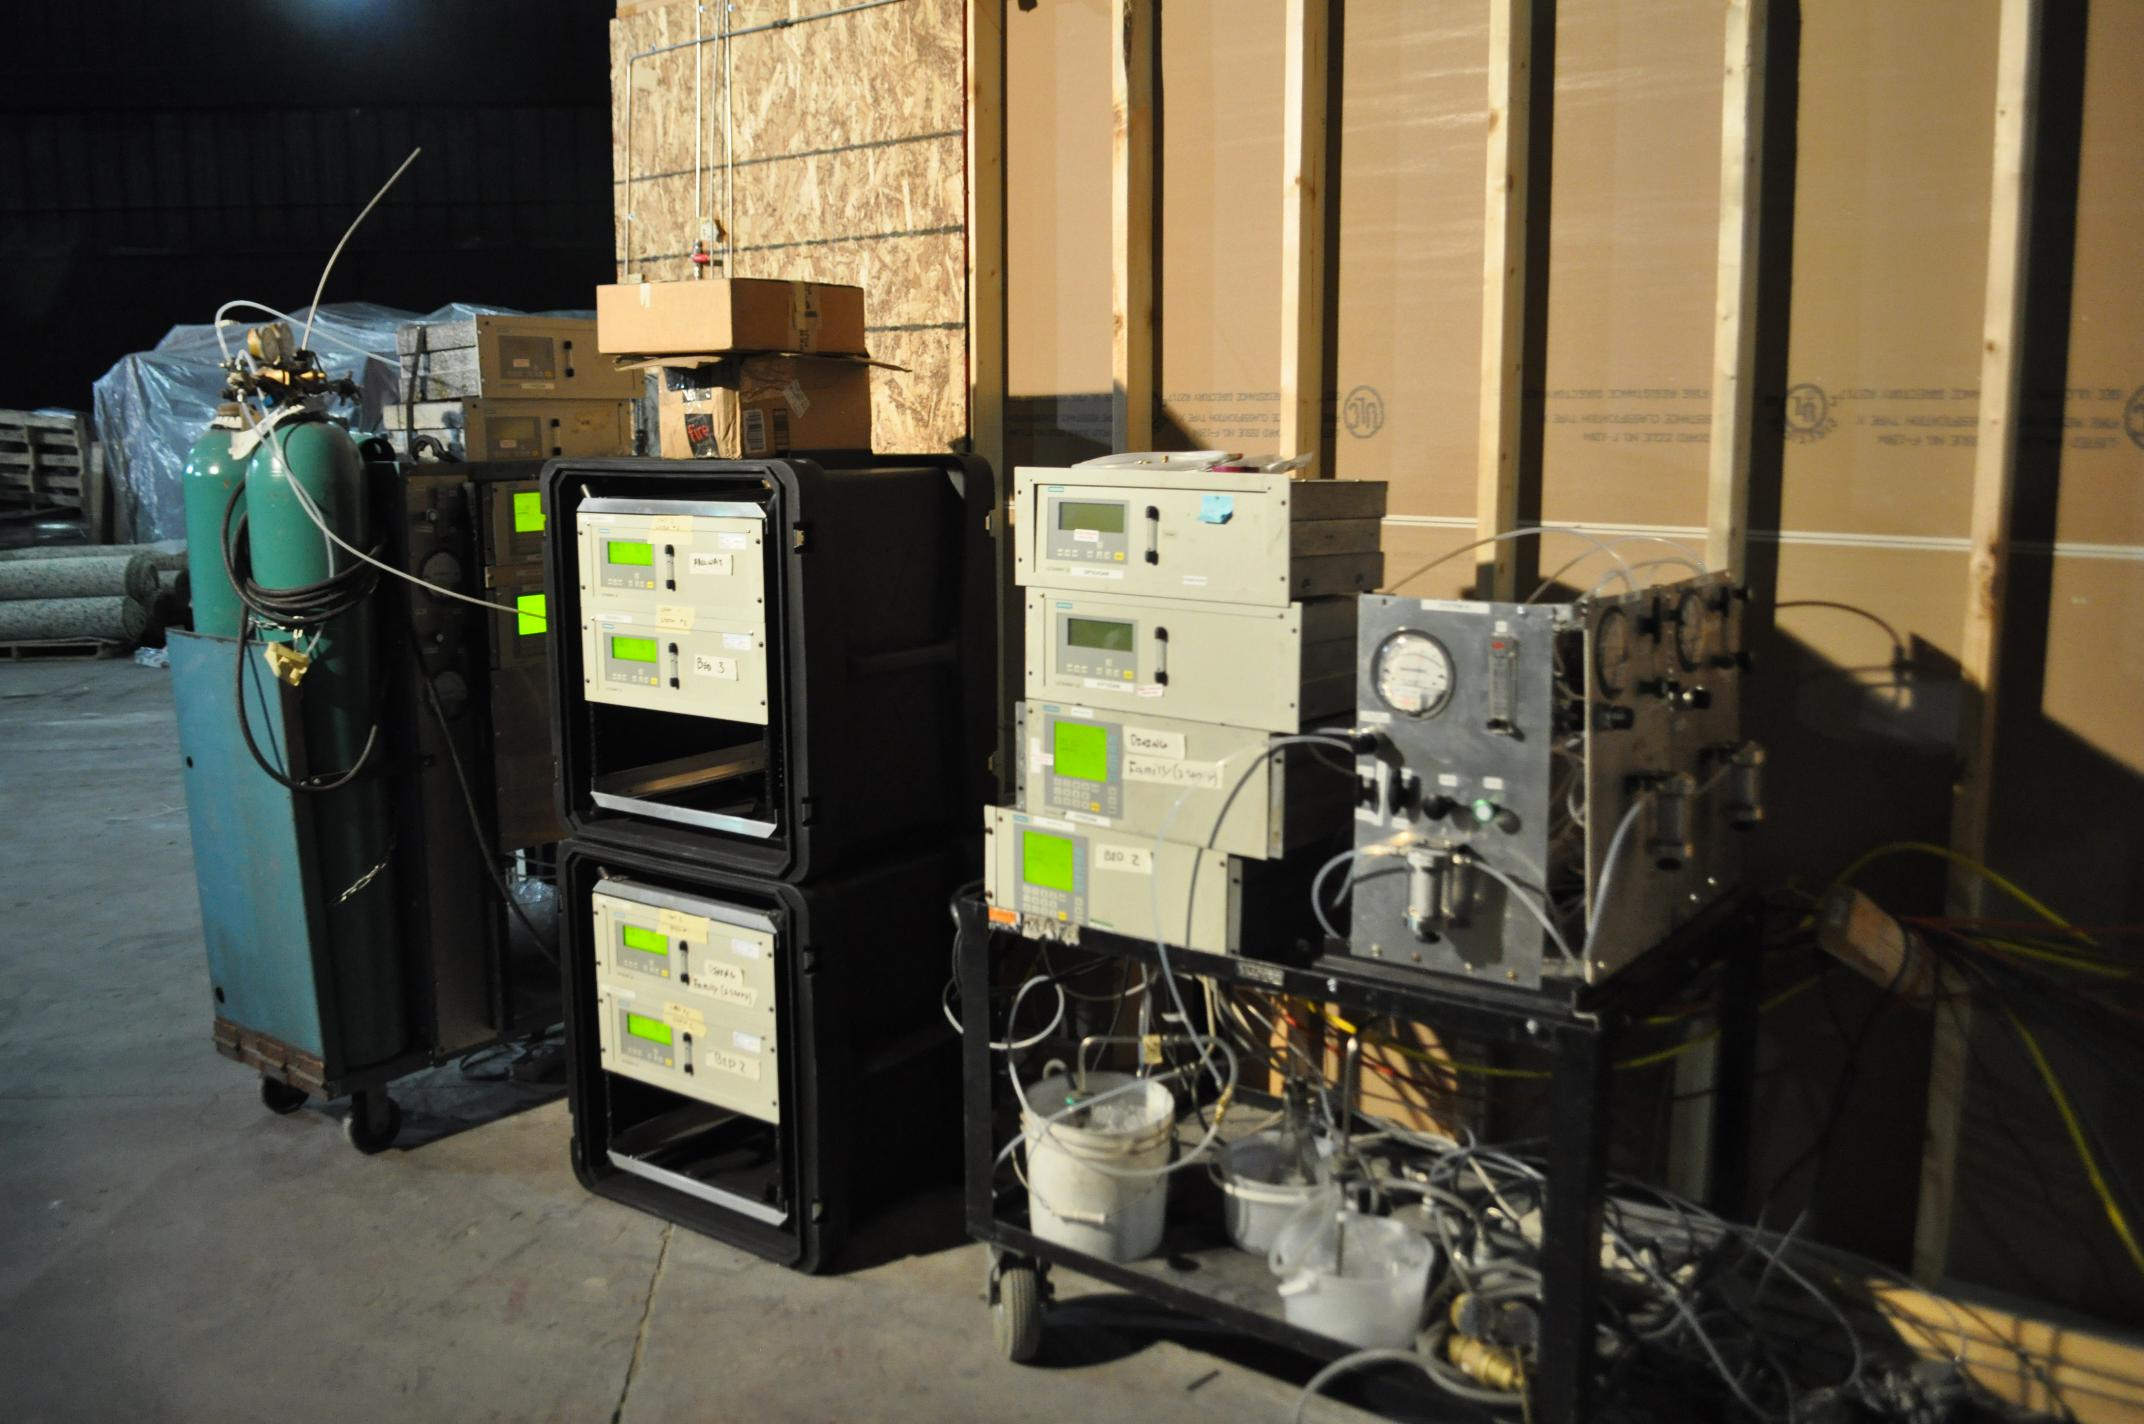
\includegraphics[width = 2in]{0_Images/Instrumentation/Gas_Analyzer/GasAnalyzers.jpg}
		\subcaption{Gas Analyzer}
	\end{minipage}
	\caption{Gas Analyser Configuration}
	\label{fig:GasAnalyzers}

\end{figure}

All data was logged through the use of a national instruments data acquisition system incorporating a SCXI-1001 chassis with 8 SCXI-1102C 32-Channel modules (Figure \ref{fig:DataSystem}). The system is configured for a total of 256 channels capable of reading values between 0-10~volts DC. Values are recorded once a second and translated to quantities of interest through the use of LabVIEW software specifically programmed for use with the system. Data was sampled at 1~hz across all channels.

\begin{figure}[H]
	\centering
	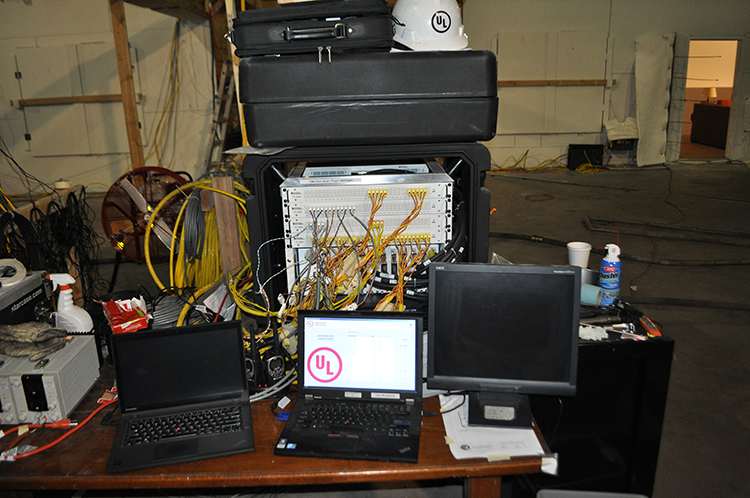
\includegraphics[width = 4in]{0_Images/Instrumentation/DataSystem.jpg}
	\caption{Data Acquisition System}
	\label{fig:DataSystem}
\end{figure}

\clearpage

\section{Measurement Locations}

In order to collect the data needed for this analysis, sensors were installed and measurements were recorded throughout each structure. The measurement locations varied dependent on the structure and desired information.

\clearpage

\section{Equipment Utilized}

In order to ensure the data collected and associated results were applicable to the majority of the fire servce, our technical panel was tasked with creating a list of represetative nozzles, specified flows/pressures, and hose line techniques. All of these variables were tested during both the air entrainment and water distribution experiments; however, several other aspects were held constant such as the length and diameter of hoseline, which were [hose length]~ft and 1.75~in, respectively. The nozzles utilized during these experiments are listed in Table~\ref{table:nozzle_selection} below.

\begin{table}[H]
\caption{Nozzle Selection }
\centering
\begin{tabular}{|l|c|c|c|}
\hline
Nozzle 		& Tip (in) 	& Nozzle Pressure (psi)	& Approximate Flow Rate (gpm) \\ \hline \hline
Smooth Bore & 	7/8 	& 	50 					& 160 \\ \hline
Combination & 	N/A 	& 	75 					& 150 \\ \hline
\end{tabular}
\label{table:nozzle_selection}
\end{table}

\clearpage

\section{Tactics Utilized}

% \begin{table}[H]
% 	\centering
% 	\caption{Tactics Utilized}
% 	\begin{tabular}{|c|c|} 
% 		\hline
% 		Shutdown \& Move & Flow \& Move & Transitional Attack \\ \hline \hline
% 		Front Door Open & Front Door Open \\ \hline
% 		Read of Conditions & Read of Conditions \\ \hline
% 		Attack Team Entry & Attack Team Entry\\ \hline
% 		Burst Suppression - "Check for Return" & Burst Suppression - "Check for Return" \\ \hline
% 		Position at start of hallway and begin flowing & Position at start of hallway and flow from fixed position (5-10 sec) \\ \hline
% 		Flow down hallway from close to far in a wall-ceiling-wall pattern while advancing until final room suppression & Flow from middle of hallway (5-10 sec) \\ \hline
% 		 & Final Room Suppression at End of Hall
% 	\end{tabular}
% 	\label{Table:Tactics}
% \end{table}

\paragraph{Shutdown \& Move Advancement}



\paragraph{Flow \& Move Advancement}



\paragraph{Transitional Attack}



\chapter{Full-Scale Residential Fire Experiments}

\section{Interior}
\subsection{No Ventilation}

\begin{figure}[H]
	\centering
	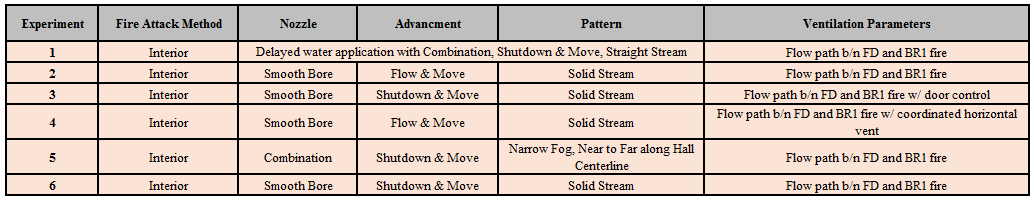
\includegraphics[width=7in]{Figures/General/Exp1to6.png}
	\caption{Experiments 1 through 6}
	\label{fig:Exp1to6}
\end{figure}

% \begin{table}[!ht]
% \caption{Experiments 1 through 6}
% \small
% \centering
% \begin{tabular}{cccccc}
% \toprule
% \textbf{Experiment} & \textbf{Fire Attack} 	& \textbf{Nozzle} 	& \textbf{Advancement} 	& \textbf{Pattern}	& \textbf{Ventilation Parameters} \\ 
% 					& \textbf{Method}	   	& & & & \\
% \midrule
%  	1 				& 	Interior 		  	& Combination 		& Delayed application 	& Straight Stream\multicolumn{3}{l}{Delayed water application w/ combination;} & Flow path between FD and BR1 fire \\
%  					& 						& \multicolumn{3}{l}{shutdown \& move; straight stream} & \\
%  	2 				& 	Interior 			& Smooth Bore 		& 	Flow \& Move 		&  	Solid Stream 	& 	Flow path between FD and BR1 fire \\
% \bottomrule
% \end{tabular}
% \label{table:exp_1_to_6}
% \end{table}

\begin{figure}[H]
	\centering
	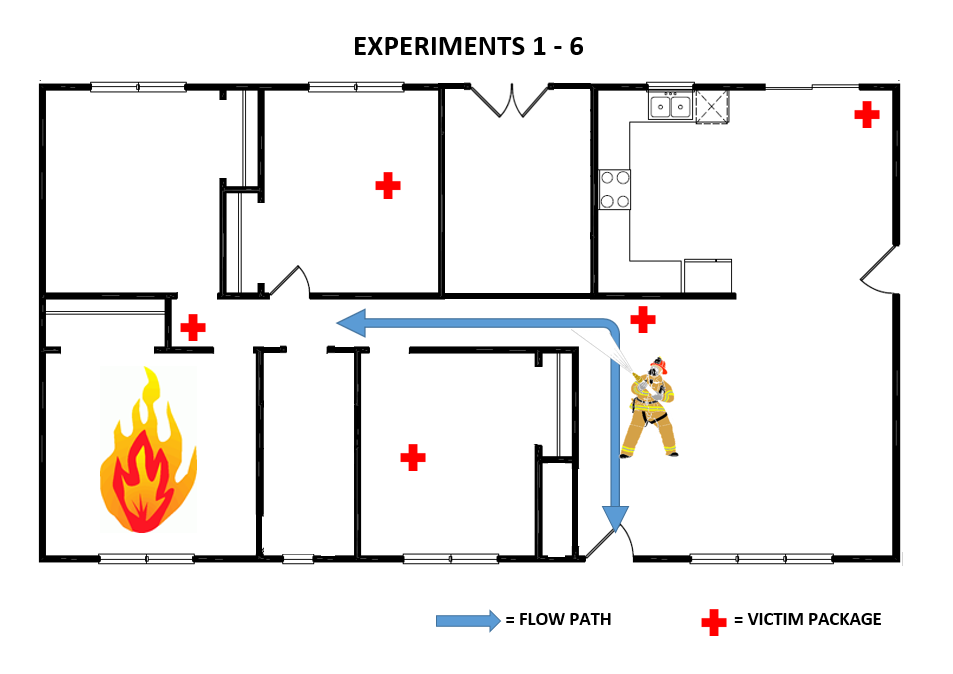
\includegraphics[width=5in]{Figures/General/Exps1through6.png}
	\caption{Configuration for Experiments 1 through 6}
	\label{fig:ExpConfig1to6}
\end{figure}

\clearpage

\paragraph{Experiment 1} \mbox{}

This experiment is intended to examine the fire dynamics in a typical single-story structure with delayed water application. The fire is ignited in Bedroom 1. The fire develops and eventually becomes ventilation limited. The front door is opened simulating fire department arrival and establishing a flow path between the front door and the bedroom. Once the fire reaches steady state, suppression will be via the front door with a combination nozzle on straight stream. The nozzle will be shutdown for line advancement. 

Figure~\ref{fig:ExpConfig1to6} shows the configuration of the structure and Table~\ref{Table:Exp1Interventions} shows at what times interventions were performed. 

The results of Experiment 1 can be found in Appendix~\ref{App:Exp1Results}. To view the full experiment video \href{https://youtu.be/gl8rc1Nsl1k}{Click Here}.

\begin{table}[H]
	\centering
	\caption{Experiment 1 Interventions}
	\begin{tabular}{|c|c|} 
		\hline
		Time & Intervention \\ \hline \hline
		00:00 & Ignition - Bedroom \\ \hline
		08:17 & Front Door Open \\ \hline
		27:47 & Attack Team Enters\\ \hline
		27:54 & Hallway Suppression \\ \hline
		42:19 & End Experiment\\ \hline
	\end{tabular}
	\label{Table:Exp1Interventions}
\end{table}

\clearpage

\paragraph{Experiment 2} \mbox{}

Experiment 2 is intended to examine the fire dynamics in a single-story structure where suppression is conducted with a smooth bore nozzle, flowing while moving. The fire is ignited in bedroom 1. The fire develops and reaches steady state at which point the front door is opened, simulating fire department arrival and establishing a flow path between the front door and the bedroom. An interior fire attack is initiated through the front door, utilizing a smooth bore nozzle, flowing while moving. 

Figure~\ref{fig:ExpConfig1to6} shows the configuration of the structure and Table~\ref{Table:Exp2Interventions} shows at what times interventions were performed. 

The results of Experiment 2 can be found in Appendix~\ref{App:Exp2Results}. To view the full experiment video \href{https://youtu.be/gl8rc1Nsl1k}{Click Here}.

\begin{table}[H]
	\centering
	\caption{Experiment 2 Interventions}
	\begin{tabular}{|c|c|} 
		\hline
		Time & Intervention \\ \hline \hline
		00:00 & Ignition - Bedroom \\ \hline
		07:05 & Front Door Open \\ \hline
		07:18 & Attack Team Enters\\ \hline
		07:23 & Burst Suppression \\ \hline 
		07:36 & Hallway Suppression \\ \hline
		18:02 & End Experiment\\ \hline
	\end{tabular}
	\label{Table:Exp2Interventions}
\end{table}

\clearpage

\paragraph{Experiment 3} \mbox{}

Experiment 3 is intended to examine the fire dynamics in a single-story structure where suppression is conducted with a solid stream and the door is controlled immediately following entry. The fire is ignited in the bedroom 1. The fire develops and becomes ventilation limited. Once this happens, the front door is opened, simulating fire department arrival, and establishing a flow path between the front door and the bedroom. An interior fire attack is initiated through the front door, utilizing a solid stream pattern. After the attack team enters, the door is closed to the width of the hose line in an effort to limit the amount of fresh air supplied to the fire. The water flow will be shutdown while the hose line is moving.

Figure~\ref{fig:ExpConfig1to6} shows the configuration of the structure and Table~\ref{Table:Exp3Interventions} shows at what times interventions were performed. 

The results of Experiment 3 can be found in Appendix~\ref{App:Exp3Results}. To view the full experiment video \href{https://youtu.be/gl8rc1Nsl1k}{Click Here}.

\begin{table}[H]
	\centering
	\caption{Experiment 3 Interventions}
	\begin{tabular}{|c|c|} 
		\hline
		Time & Intervention \\ \hline \hline
		00:00 & Ignition - Bedroom \\ \hline
		08:26 & Front Door Open \\ \hline
		08:28 & Attack Team Enters\\ \hline
		08:32 & Burst Suppression \\ \hline 
		08:45 & Hallway Suppression \\ \hline
		19:09 & End Experiment\\ \hline
	\end{tabular}
	\label{Table:Exp3Interventions}
\end{table}

\clearpage

\paragraph{Experiment 4} \mbox{}

Experiment 4 is intended to examine the fire dynamics of a fire in a single-story structure where suppression is conducted with a straight stream pattern. The fire is ignited in bedroom 1. The fire develops and eventually becomes ventilation limited. Once this happens, the front door is opened, simulating fire department arrival and establishing a flow path between the front door and bedroom 1. An interior fire attack is initiated through the front door, utilizing a solid stream pattern. That is flowing while the hose line is moving. Suppression is coordinated with horizontal ventilation of the bedroom 1 window. 

Figure~\ref{fig:ExpConfig1to6} shows the configuration of the structure and Table~\ref{Table:Exp4Interventions} shows at what times interventions were performed. 

The results of Experiment 4 can be found in Appendix~\ref{App:Exp4Results}. To view the full experiment video \href{https://youtu.be/gl8rc1Nsl1k}{Click Here}.

\begin{table}[H]
	\centering
	\caption{Experiment 4 Interventions}
	\begin{tabular}{|c|c|} 
		\hline
		Time & Intervention \\ \hline \hline
		00:00 & Ignition - Bedroom \\ \hline
		08:25 & Front Door Open \\ \hline
		08:38 & Attack Team Enters\\ \hline
		08:43 & Burst Suppression \\ \hline
		08:43 & Bedroom 1 Window Open \\ \hline 
		08:54 & Hallway Suppression \\ \hline
		15:23 & End Experiment\\ \hline
	\end{tabular}
	\label{Table:Exp4Interventions}
\end{table}

\clearpage

\paragraph{Experiment 5} \mbox{}

Experiment 5 is intended to examine the fire dynamics in a single-story structure where suppression is conducted with a narrow fog pattern. The fire is ignited in the bedroom 1. The fire develops and becomes ventilation limited. Once this happens, the front door is opened, simulating fire department arrival and establishing a flow path between the front door and bedroom 1. An interior fire attack is initiated through the front door, utilizing a narrow fog pattern. Water will be flowing while the hose line is advanced.  

Figure~\ref{fig:ExpConfig1to6} shows the configuration of the structure and Table~\ref{Table:Exp5Interventions} shows at what times interventions were performed. 

The results of Experiment 5 can be found in Appendix~\ref{App:Exp5Results}. To view the full experiment video \href{https://youtu.be/gl8rc1Nsl1k}{Click Here}.

\begin{table}[H]
	\centering
	\caption{Experiment 5 Interventions}
	\begin{tabular}{|c|c|} 
		\hline
		Time & Intervention \\ \hline \hline
		00:00 & Ignition - Bedroom \\ \hline
		06:57 & Front Door Open \\ \hline
		07:09 & Attack Team Enters\\ \hline
		07:16 & Burst Suppression \\ \hline 
		07:27 & Hallway Suppression \\ \hline
		17:54 & End Experiment\\ \hline
	\end{tabular}
	\label{Table:Exp5Interventions}
\end{table}

\clearpage

\paragraph{Experiment 6} \mbox{}

Experiment 6 is intended to examine the fire dynamics in a single-story structure where suppression is conducted with a solid stream pattern. The fire is ignited in bedroom 1. The fire develops and becomes ventilation limited. Once this happens, the front door is opened, simulating fire department arrival and establishing a flow path between the front door and bedroom 1. An interior fire attack is initiated through the front door, utilizing a solid stream pattern. The water flow will be shutdown while the hose line is moving. 

Figure~\ref{fig:ExpConfig1to6} shows the configuration of the structure and Table~\ref{Table:Exp6Interventions} shows at what times interventions were performed. 

The results of Experiment 6 can be found in Appendix~\ref{App:Exp6Results}. To view the full experiment video \href{https://youtu.be/gl8rc1Nsl1k}{Click Here}.

\begin{table}[H]
	\centering
	\caption{Experiment 6 Interventions}
	\begin{tabular}{|c|c|} 
		\hline
		Time & Intervention \\ \hline \hline
		00:00 & Ignition - Bedroom \\ \hline
		07:58 & Front Door Open \\ \hline
		08:13 & Attack Team Enters\\ \hline
		08:18 & Burst Suppression \\ \hline 
		08:27 & Hallway Suppression \\ \hline
		14:38 & End Experiment\\ \hline
	\end{tabular}
	\label{Table:Exp6Interventions}
\end{table}

\clearpage

\subsection{Single Room - Single Vent}

\begin{figure}[H]
	\centering
	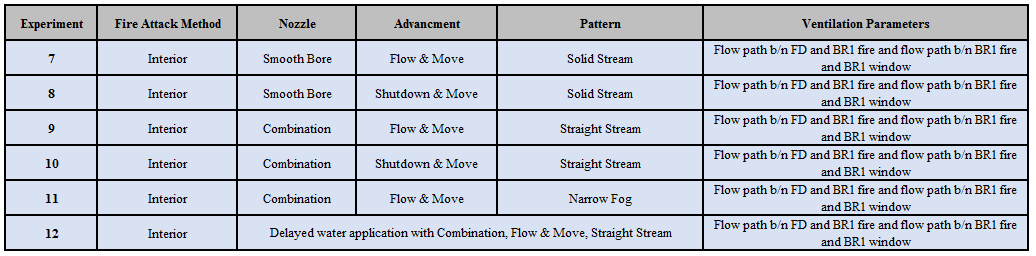
\includegraphics[width=7in]{Figures/General/Exp7to12.png}
	\caption{Experiments 7 to 12}
	\label{fig:Exp7to12}
\end{figure}

\begin{figure}[H]
	\centering
	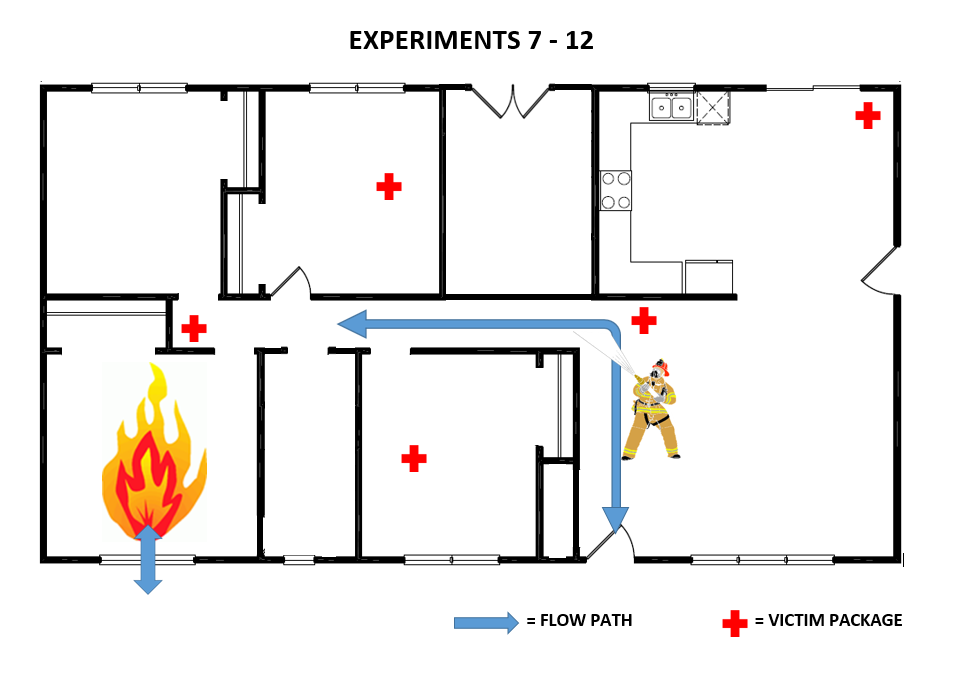
\includegraphics[width=5in]{Figures/General/Exps7through12.png}
	\caption{Configurations for Experiments 7 to 12}
	\label{fig:ExpConfig7to12}
\end{figure}

\clearpage

\paragraph{Experiment 7} \mbox{}

Experiment 7 is intended to examine the fire dynamics in a single-story structure where suppression is conducted with a solid stream pattern. The fire is ignited in the bedroom 1. The fire develops and becomes ventilation limited. Once this happens, the front door is opened, simulating fire department arrival and establishing two flow paths: One between the front door and the bedroom fire and the other between the bedroom window and the bedroom fire. An interior fire attack is initiated through the front door, utilizing a solid stream pattern. Water will be flowing while the hose line is advanced. 

Figure~\ref{fig:ExpConfig7to12} shows the configuration of the structure and Table~\ref{Table:Exp7Interventions} shows at what times interventions were performed. 

The results of Experiment 7 can be found in Appendix~\ref{App:Exp7Results}. To view the full experiment video \href{https://youtu.be/gl8rc1Nsl1k}{Click Here}.

\begin{table}[H]
	\centering
	\caption{Experiment 7 Interventions}
	\begin{tabular}{|c|c|} 
		\hline
		Time & Intervention \\ \hline \hline
		00:00 & Ignition - Bedroom \\ \hline
		05:55 & Front Door Open \\ \hline
		06:07 & Attack Team Enters\\ \hline
		06:12 & Burst Suppression \\ \hline 
		06:22 & Hallway Suppression \\ \hline
		12:26 & End Experiment\\ \hline
	\end{tabular}
	\label{Table:Exp7Interventions}
\end{table}

\clearpage

\paragraph{Experiment 8} \mbox{}

Experiment 8 is intended to examine the fire dynamics in a single-story structure where suppression is conducted with a solid stream pattern. The fire is ignited in the bedroom 1. The fire develops and becomes ventilation limited. Once this happens, the front door is opened, simulating fire department arrival and establishing two flow paths: One between the front door and the bedroom fire and the other between the bedroom window and the bedroom fire. An interior fire attack is initiated through the front door, utilizing a solid stream The water flow will be shutdown while the hose line is moving. 

Figure~\ref{fig:ExpConfig7to12} shows the configuration of the structure and Table~\ref{Table:Exp8Interventions} shows at what times interventions were performed. 

The results of Experiment 8 can be found in Appendix~\ref{App:Exp8Results}. To view the full experiment video \href{https://youtu.be/gl8rc1Nsl1k}{Click Here}.

\begin{table}[H]
	\centering
	\caption{Experiment 8 Interventions}
	\begin{tabular}{|c|c|} 
		\hline
		Time & Intervention \\ \hline \hline
		00:00 & Ignition - Bedroom \\ \hline
		05:26 & Front Door Open \\ \hline
		05:40 & Attack Team Enters\\ \hline
		05:45 & Burst Suppression \\ \hline 
		05:54 & Hallway Suppression \\ \hline
		11:57 & End Experiment\\ \hline
	\end{tabular}
	\label{Table:Exp8Interventions}
\end{table}

\clearpage

\paragraph{Experiment 9} \mbox{}

Experiment 9 is intended to examine the fire dynamics in a single-story structure where suppression is conducted with a straight stream pattern. The fire is ignited in the bedroom 1. The fire develops and becomes ventilation limited. Once this happens, the front door is opened, simulating fire department arrival and establishing two flow paths: One between the front door and the bedroom fire and the other between the bedroom window and the bedroom fire. An interior fire attack is initiated through the front door, utilizing a straight stream Water will be flowing while the hose line is advanced. 

Figure~\ref{fig:ExpConfig7to12} shows the configuration of the structure and Table~\ref{Table:Exp9Interventions} shows at what times interventions were performed. 

The results of Experiment 9 can be found in Appendix~\ref{App:Exp9Results}. To view the full experiment video \href{https://youtu.be/gl8rc1Nsl1k}{Click Here}.

\begin{table}[H]
	\centering
	\caption{Experiment 9 Interventions}
	\begin{tabular}{|c|c|} 
		\hline
		Time & Intervention \\ \hline \hline
		00:00 & Ignition - Bedroom \\ \hline
		05:27 & Front Door Open \\ \hline
		05:38 & Attack Team Enters\\ \hline
		05:45 & Burst Suppression \\ \hline 
		05:53 & Hallway Suppression \\ \hline
		11:59 & End Experiment\\ \hline
	\end{tabular}
	\label{Table:Exp9Interventions}
\end{table}

\clearpage

\paragraph{Experiment 10} \mbox{}

Experiment 10 is intended to examine the fire dynamics in a single-story structure where suppression is conducted with a straight stream. The fire is ignited in the bedroom 1. The fire develops and becomes ventilation limited. Once this happens, the front door is opened, simulating fire department arrival and establishing two flow paths: One between the front door and the bedroom fire and the other between the bedroom window and the bedroom fire. An interior fire attack is initiated through the front door, utilizing a straight stream The water flow will be shutdown while the hose line is moving. 

Figure~\ref{fig:ExpConfig7to12} shows the configuration of the structure and Table~\ref{Table:Exp10Interventions} shows at what times interventions were performed. 

The results of Experiment 10 can be found in Appendix~\ref{App:Exp10Results}. To view the full experiment video \href{https://youtu.be/gl8rc1Nsl1k}{Click Here}.

\begin{table}[H]
	\centering
	\caption{Experiment 10 Interventions}
	\begin{tabular}{|c|c|} 
		\hline
		Time & Intervention \\ \hline \hline
		00:00 & Ignition - Bedroom \\ \hline
		05:27 & Front Door Open \\ \hline
		05:39 & Attack Team Enters\\ \hline
		05:45 & Burst Suppression \\ \hline 
		05:54 & Hallway Suppression \\ \hline
		12:07 & End Experiment\\ \hline
	\end{tabular}
	\label{Table:Exp10Interventions}
\end{table}

\clearpage

\paragraph{Experiment 11} \mbox{}

Experiment 11 is intended to examine the fire dynamics in a single-story structure where suppression is conducted with a fog stream pattern. The fire is ignited in bedroom 1. The fire develops and becomes ventilation limited. Once this happens, the front door is opened, simulating fire department arrival and establishing two flow paths: One between the front door and the bedroom fire and the other between the bedroom window and the bedroom fire. An interior fire attack is initiated through the front door, utilizing a narrow fog stream pattern. Water will be flowing while the hose line is advanced.  

Figure~\ref{fig:ExpConfig7to12} shows the configuration of the structure and Table~\ref{Table:Exp11Interventions} shows at what times interventions were performed. 

The results of Experiment 11 can be found in Appendix~\ref{App:Exp11Results}. To view the full experiment video \href{https://youtu.be/gl8rc1Nsl1k}{Click Here}.

\begin{table}[H]
	\centering
	\caption{Experiment 11 Interventions}
	\begin{tabular}{|c|c|} 
		\hline
		Time & Intervention \\ \hline \hline
		00:00 & Ignition - Bedroom \\ \hline
		06:20 & Front Door Open \\ \hline
		06:32 & Attack Team Enters\\ \hline
		06:38 & Burst Suppression \\ \hline 
		06:49 & Hallway Suppression \\ \hline
		12:24 & End Experiment\\ \hline
	\end{tabular}
	\label{Table:Exp11Interventions}
\end{table}

\clearpage

\paragraph{Experiment 12} \mbox{}

This experiment is intended to examine the fire dynamics in a typical single-story structure with delayed water application. The fire is ignited in bedroom 1 with the bedroom 1 window open. Once the fire reaches steady state, the front door is opened, simulating fire department arrival. This establishes two flow paths: one between the front door and bedroom 1 and another between the bedroom 1 window and the bedroom. Once the fire reaches steady state again the suppression is initiated via an interior attack with a combination nozzle set to straight stream. The water flow will be shutdown while the hose line is moving.  

Figure~\ref{fig:ExpConfig7to12} shows the configuration of the structure and Table~\ref{Table:Exp12Interventions} shows at what times interventions were performed. 

The results of Experiment 12 can be found in Appendix~\ref{App:Exp12Results}. To view the full experiment video \href{https://youtu.be/gl8rc1Nsl1k}{Click Here}.

\begin{table}[H]
	\centering
	\caption{Experiment 12 Interventions}
	\begin{tabular}{|c|c|} 
		\hline
		Time & Intervention \\ \hline \hline
		00:00 & Ignition - Bedroom \\ \hline
		05:57 & Front Door Open \\ \hline
		13:29 & Attack Team Enters\\ \hline
		13:32 & Burst Suppression \\ \hline 
		13:40 & Hallway Suppression \\ \hline
		28:46 & End Experiment\\ \hline
	\end{tabular}
	\label{Table:Exp12Interventions}
\end{table}

\clearpage

\subsection{Two Room - Two Vent}

\begin{figure}[H]
	\centering
	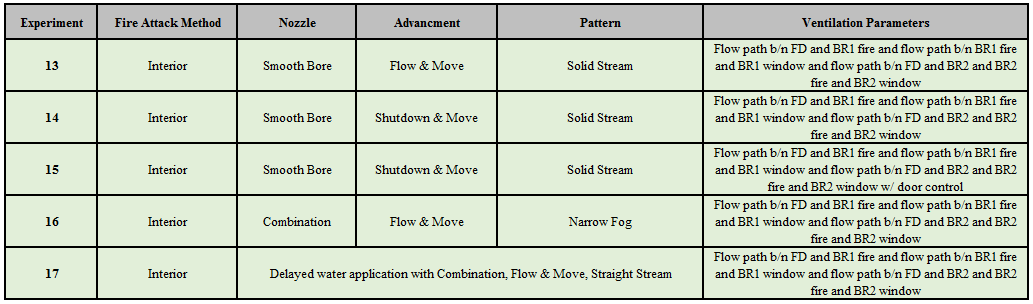
\includegraphics[width=7in]{Figures/General/Exp13to17.png}
	\caption{Experiments 13 to 17}
	\label{fig:Exp13to17}
\end{figure}

\begin{figure}[H]
	\centering
	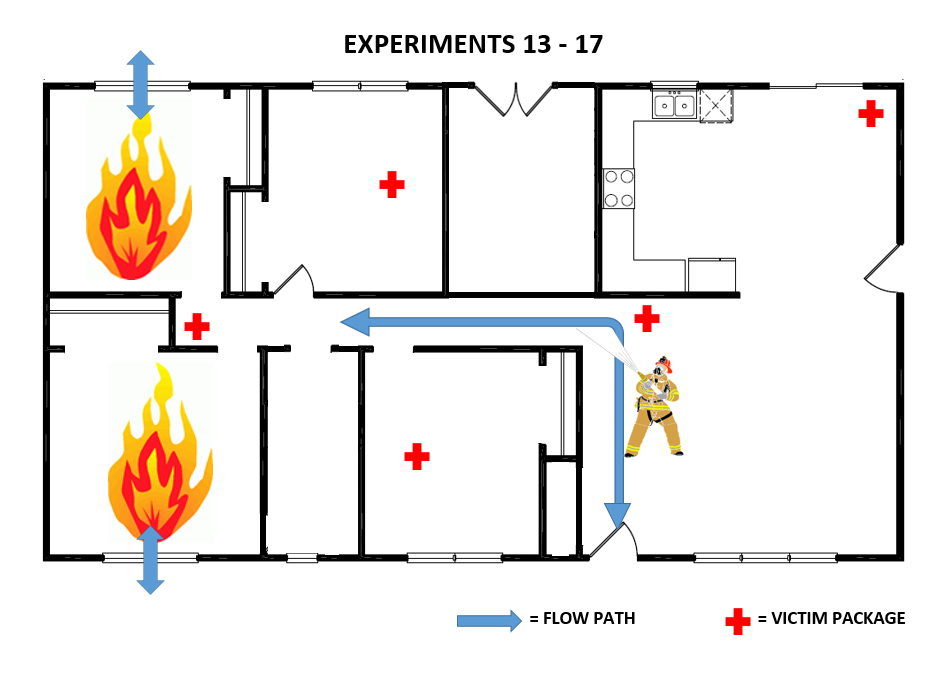
\includegraphics[width=5in]{Figures/General/Exps13through17.png}
	\caption{Configurations for Experiments 13 to 17}
	\label{fig:ExpConfig13to17}
\end{figure}

\clearpage

\paragraph{Experiment 13} \mbox{}

Experiment 13 is intended to examine a 2-bedroom fire in a single-story structure where suppression is conducted with a solid stream pattern. The fire is ignited simultaneously in bedroom 1 and bedroom 2. The fire develops and becomes ventilation limited. Once this happens, the front door is opened, simulating fire department arrival. These actions create flow paths between the front door and each fire bedroom and between each bedroom window and the fire bedrooms. An interior fire attack is initiated through the front door, utilizing a solid stream pattern. Water will be flowing while the hose line is advanced.  

Figure~\ref{fig:ExpConfig13to17} shows the configuration of the structure and Table~\ref{Table:Exp13Interventions} shows at what times interventions were performed. 

The results of Experiment 13 can be found in Appendix~\ref{App:Exp13Results}. To view the full experiment video \href{https://youtu.be/gl8rc1Nsl1k}{Click Here}.

\begin{table}[H]
	\centering
	\caption{Experiment 13 Interventions}
	\begin{tabular}{|c|c|} 
		\hline
		Time & Intervention \\ \hline \hline
		00:00 & Ignition - Bedroom \\ \hline
		05:39 & Front Door Open \\ \hline
		05:52 & Attack Team Enters\\ \hline
		05:57 & Burst Suppression \\ \hline 
		06:11 & Hallway Suppression \\ \hline
		12:06 & End Experiment\\ \hline
	\end{tabular}
	\label{Table:Exp13Interventions}
\end{table}

\clearpage

\paragraph{Experiment 14} \mbox{}

Experiment 14 is intended to examine a 2-bedroom fire in a single-story structure where suppression is conducted with a solid stream. The fire is ignited simultaneously in the bedroom 1 and bedroom 2. The fire develops and becomes ventilation limited. Once this happens, the front door is opened simulating fire department arrival. These actions create flow paths between the front door and each fire bedroom and between each bedroom window and the fire bedrooms. An interior fire attack is initiated through the front door, utilizing a solid stream. The water flow will be shutdown while the hose line is moving. 

Figure~\ref{fig:ExpConfig13to17} shows the configuration of the structure and Table~\ref{Table:Exp14Interventions} shows at what times interventions were performed. 

The results of Experiment 14 can be found in Appendix~\ref{App:Exp14Results}. To view the full experiment video \href{https://youtu.be/gl8rc1Nsl1k}{Click Here}.

\begin{table}[H]
	\centering
	\caption{Experiment 14 Interventions}
	\begin{tabular}{|c|c|} 
		\hline
		Time & Intervention \\ \hline \hline
		00:00 & Ignition - Bedroom \\ \hline
		06:26 & Front Door Open \\ \hline
		06:39 & Attack Team Enters\\ \hline
		06:43 & Burst Suppression \\ \hline 
		06:50 & Hallway Suppression \\ \hline
		15:05 & End Experiment\\ \hline
	\end{tabular}
	\label{Table:Exp14Interventions}
\end{table}

\clearpage

\paragraph{Experiment 15} \mbox{}

Experiment 15 is intended to examine a 2-bedroom fire in a single-story structure where suppression is conducted with a solid stream pattern. The fire is ignited simultaneously in bedroom 1 and bedroom 2. The fire develops and becomes ventilation limited. Once this happens, the front door is opened simulating fire department arrival. This action create flow paths between the front door and each fire bedroom and between each bedroom window and the fire bedrooms. An interior fire attack is initiated through the front door, utilizing a solid stream . After the attack team enters, the door is closed to the width of the hose line in an effort to limit the amount of fresh air supplied to the fire. The water flow will be shutdown while the hose line is moving.

Figure~\ref{fig:ExpConfig13to17} shows the configuration of the structure and Table~\ref{Table:Exp15Interventions} shows at what times interventions were performed. 

The results of Experiment 15 can be found in Appendix~\ref{App:Exp15Results}. To view the full experiment video \href{https://youtu.be/gl8rc1Nsl1k}{Click Here}.

\begin{table}[H]
	\centering
	\caption{Experiment 15 Interventions}
	\begin{tabular}{|c|c|} 
		\hline
		Time & Intervention \\ \hline \hline
		00:00 & Ignition - Bedroom \\ \hline
		05:39 & Front Door Open \\ \hline
		05:40 & Attack Team Enters\\ \hline
		05:44 & Burst Suppression \\ \hline 
		05:55 & Hallway Suppression \\ \hline
		12:06 & End Experiment\\ \hline
	\end{tabular}
	\label{Table:Exp15Interventions}
\end{table}

\clearpage

\paragraph{Experiment 16} \mbox{}

Experiment 16 is intended to examine a 2-bedroom fire in a single-story structure where suppression is conducted with a narrow fog stream. The fire is ignited simultaneously in bedroom 1 and bedroom 2. The fire develops and becomes ventilation limited. Once this happens, the front door is opened simulating fire department arrival. These actions create flow paths between the front door and each fire bedroom and between each bedroom window and the fire bedrooms. An interior fire attack is initiated through the front door, utilizing a narrow fog stream. Water will be flowing while the hose line is advanced. 

Figure~\ref{fig:ExpConfig13to17} shows the configuration of the structure and Table~\ref{Table:Exp16Interventions} shows at what times interventions were performed. 

The results of Experiment 16 can be found in Appendix~\ref{App:Exp16Results}. To view the full experiment video \href{https://youtu.be/gl8rc1Nsl1k}{Click Here}.

\begin{table}[H]
	\centering
	\caption{Experiment 16 Interventions}
	\begin{tabular}{|c|c|} 
		\hline
		Time & Intervention \\ \hline \hline
		00:00 & Ignition - Bedroom \\ \hline
		05:23 & Front Door Open \\ \hline
		05:33 & Attack Team Enters\\ \hline
		05:37 & Burst Suppression \\ \hline 
		05:54 & Hallway Suppression \\ \hline
		12:58 & End Experiment\\ \hline
	\end{tabular}
	\label{Table:Exp16Interventions}
\end{table}

\clearpage

\paragraph{Experiment 17} \mbox{}

Experiment 17 will examine a fire in a single-story structure where suppression is conducted with a straight stream, shutdown while moving. The fire is ignited in bedroom 1 and bedroom 2. The windows in bedroom 1 and 2 will be open at the start of the experiment. The fire develops and becomes ventilation limited. Once this happens, the front door will be opened, simulating fire department arrival. So at the point of fire attack flow paths exist between the front door and bedroom 1, between the bedroom 1 window and the bedroom1 , between the front door and bedroom 2, and between the bedroom 2 window and bedroom 2. 

Figure~\ref{fig:ExpConfig13to17} shows the configuration of the structure and Table~\ref{Table:Exp17Interventions} shows at what times interventions were performed. 

The results of Experiment 17 can be found in Appendix~\ref{App:Exp17Results}. To view the full experiment video \href{https://youtu.be/gl8rc1Nsl1k}{Click Here}.

\begin{table}[H]
	\centering
	\caption{Experiment 17 Interventions}
	\begin{tabular}{|c|c|} 
		\hline
		Time & Intervention \\ \hline \hline
		00:00 & Ignition - Bedroom \\ \hline
		05:27 & Front Door Open \\ \hline
		10:32 & Attack Team Enters\\ \hline
		10:36 & Burst Suppression \\ \hline 
		10:47 & Hallway Suppression \\ \hline
		23:32 & End Experiment\\ \hline
	\end{tabular}
	\label{Table:Exp17Interventions}
\end{table}

\clearpage

\section{Exterior}

\subsection{Single Room - Single Vent}

\begin{figure}[H]
	\centering
	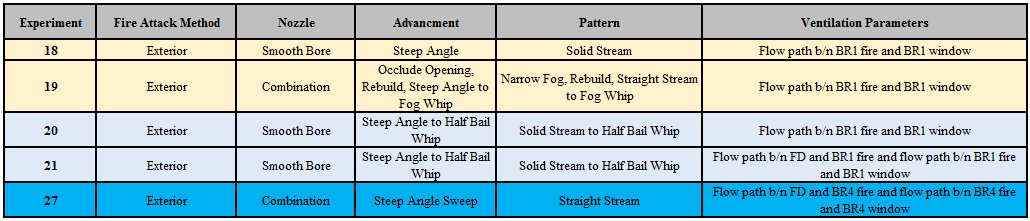
\includegraphics[width=7in]{Figures/General/Exp18to21and27.png}
	\caption{Experiments 18 through 21 and 27}
	\label{fig:Exp18to21and27}
\end{figure}

\begin{figure}[H]
	\centering
	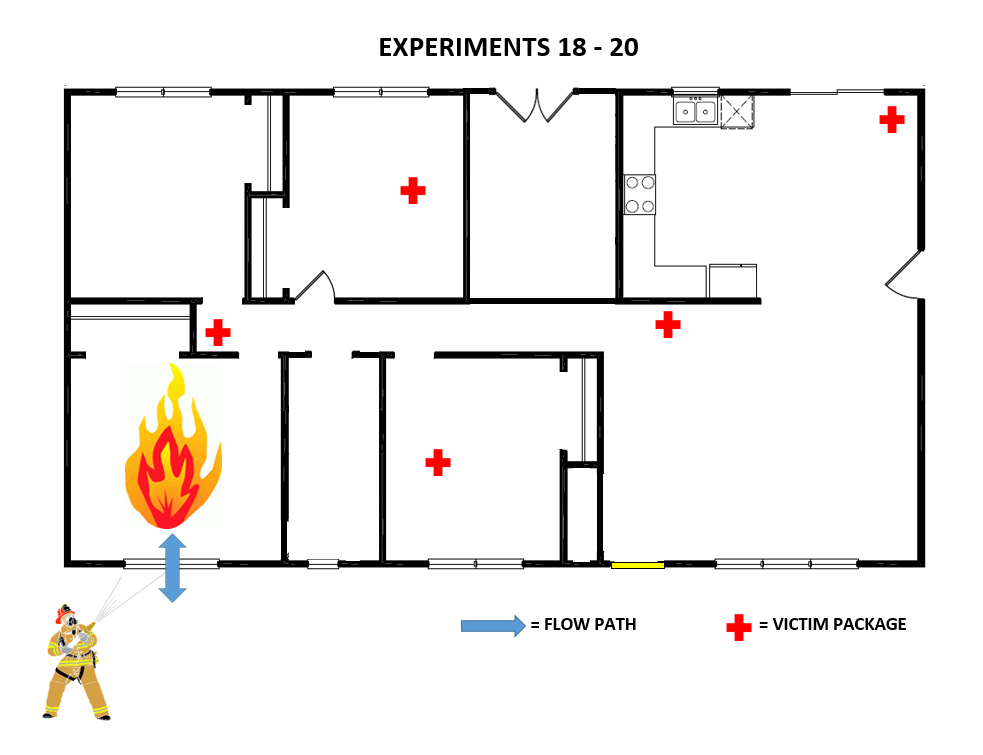
\includegraphics[width=5in]{Figures/General/Exps18through20.png}
	\caption{Configuration for Experiments 18 through 20.}
	\label{fig:ExpConfig18to20}
\end{figure}

\begin{figure}[H]
	\centering
	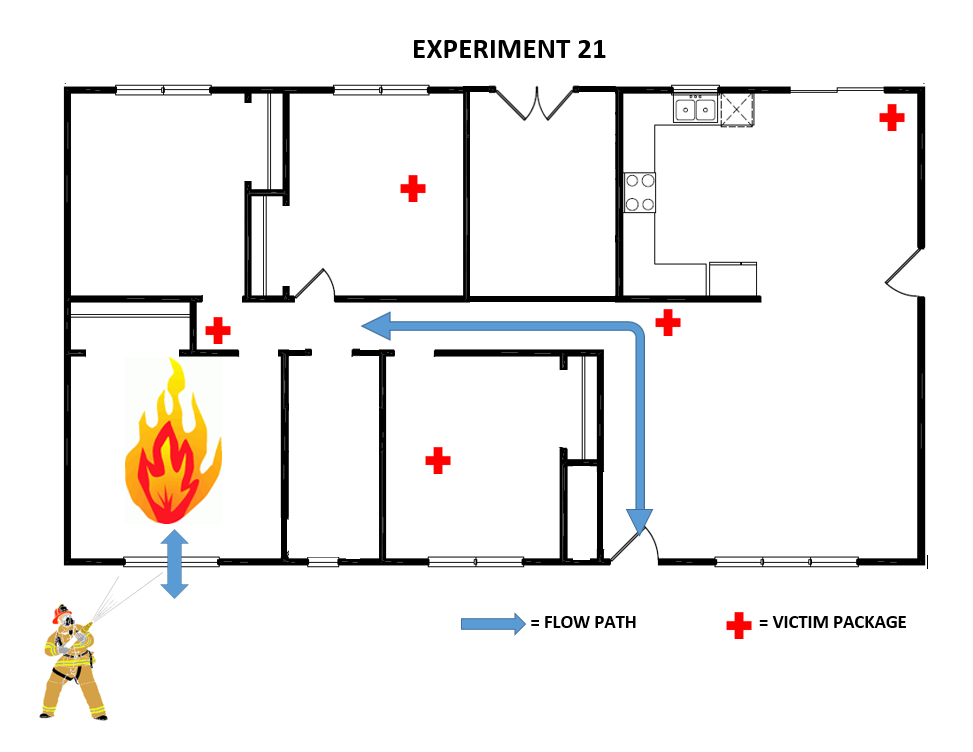
\includegraphics[width=5in]{Figures/General/Exp21.png}
	\caption{Configuration for Experiment 21.}
	\label{fig:ExpConfig21}
\end{figure}

\begin{figure}[H]
	\centering
	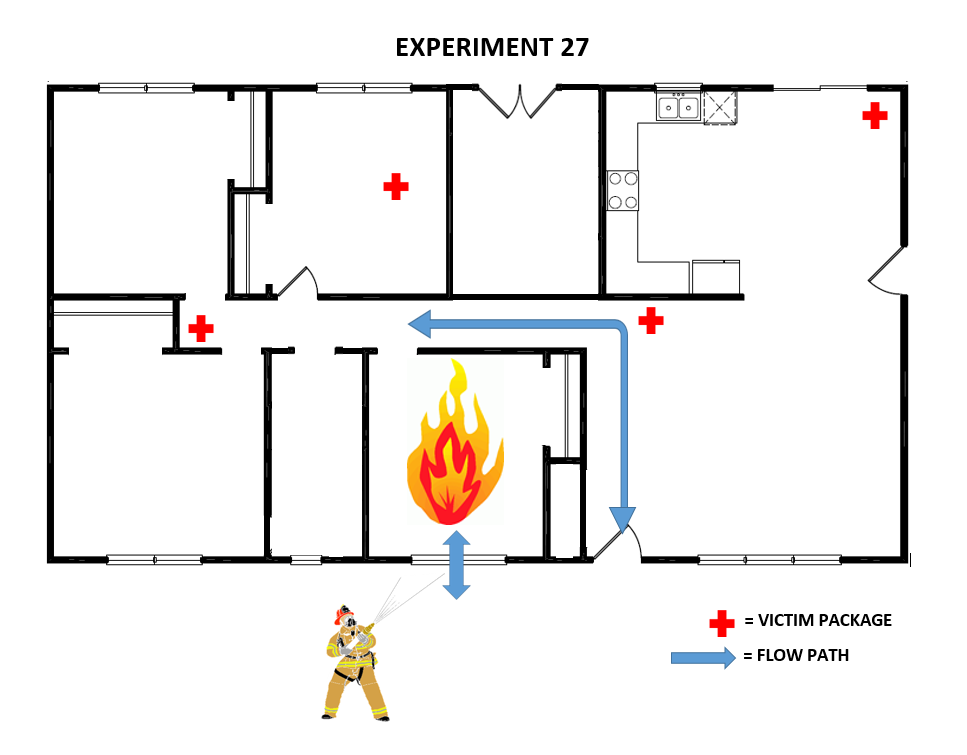
\includegraphics[width=5in]{Figures/General/Exp27.png}
	\caption{Configuration for Experiment 27.}
	\label{fig:ExpConfig27}
\end{figure}

\clearpage

\paragraph{Experiment 18} \mbox{}

Experiment 18 is intended to study a bedroom fire in a single-story structure where suppression is initiated from the exterior of the house with a straight stream. The fire is ignited in bedroom 1. As the fire develops, it transitions to a ventilation limited fire. Soon after the fire becomes ventilation limited simulating fire department arrival. Water is applied through the bedroom window, simulating a transitional attack. The exterior fire attack is conducted using a solid stream. Interior attack will be used if needed for extinguishment. 

Figure~\ref{fig:ExpConfig18to20} shows the configuration of the structure and Table~\ref{Table:Exp18Interventions} shows at what times interventions were performed. 

The results of Experiment 18 can be found in Appendix~\ref{App:Exp18Results}. To view the full experiment video \href{https://youtu.be/gl8rc1Nsl1k}{Click Here}.

\begin{table}[H]
	\centering
	\caption{Experiment 18 Interventions}
	\begin{tabular}{|c|c|} 
		\hline
		Time & Intervention \\ \hline \hline
		00:00 & Ignition - Bedroom \\ \hline
		05:24 & Exterior Suppression BR1 Window Solid Stream \\ \hline
		05:35 & Front Door Open \\ \hline
		05:42 & Attack Team Enters\\ \hline
		05:45 & Burst Suppression \\ \hline 
		06:07 & Hallway Suppression \\ \hline
		12:04 & End Experiment\\ \hline
	\end{tabular}
	\label{Table:Exp18Interventions}
\end{table}

\clearpage

\paragraph{Experiment 19} \mbox{}

Experiment 19 is intended to study a bedroom fire in a single-story structure where suppression is initiated from the exterior of the house with a narrow fog stream. The fire is ignited in bedroom 1. As the fire develops, it transitions to a ventilation limited fire. Soon after the fire becomes ventilation limited. Water is applied through the bedroom 1 window, simulating a transitional attack. The exterior fire attack is conducted using a solid stream. Interior attack will be used if needed for extinguishment. 

Figure~\ref{fig:ExpConfig18to20} shows the configuration of the structure and Table~\ref{Table:Exp19Interventions} shows at what times interventions were performed. 

The results of Experiment 19 can be found in Appendix~\ref{App:Exp19Results}. To view the full experiment video \href{https://youtu.be/gl8rc1Nsl1k}{Click Here}.

\begin{table}[H]
	\centering
	\caption{Experiment 19 Interventions}
	\begin{tabular}{|c|c|} 
		\hline
		Time & Intervention \\ \hline \hline
		00:00 & Ignition - Bedroom \\ \hline
		05:24 & Exterior Suppression BR1 Window Narrow Fog Stream \\ \hline
		08:28 & Exterior Suppression BR1 Window Straight Stream \\ \hline
		08:58 & Front Door Open \\ \hline
		09:10 & Attack Team Enters\\ \hline
		09:34 & Room Suppression \\ \hline 
		14:05 & End Experiment\\ \hline
	\end{tabular}
	\label{Table:Exp19Interventions}
\end{table}

\clearpage

\paragraph{Experiment 20} \mbox{}

This experiment is intended to study a bedroom fire in a single-story structure where suppression is initiated from the exterior of the house with a solid stream. The fire is ignited in bedroom 1. As the fire develops, it transitions to a ventilation limited fire. Soon after the fire becomes ventilation limited, the front door is open, simulating fire department arrival. Water is applied through the bedroom 1 window, simulating a transitional attack. The exterior fire attack is conducted using a solid stream. Interior attack will be used if needed for extinguishment.  

Figure~\ref{fig:ExpConfig18to20} shows the configuration of the structure and Table~\ref{Table:Exp20Interventions} shows at what times interventions were performed. 

The results of Experiment 20 can be found in Appendix~\ref{App:Exp20Results}. To view the full experiment video \href{https://youtu.be/gl8rc1Nsl1k}{Click Here}.

\begin{table}[H]
	\centering
	\caption{Experiment 20 Interventions}
	\begin{tabular}{|c|c|} 
		\hline
		Time & Intervention \\ \hline \hline
		00:00 & Ignition - Bedroom \\ \hline
		06:52 & Exterior Suppression BR1 Window Solid Stream \\ \hline
		07:24 & Front Door Open \\ \hline
		07:34 & Attack Team Enters\\ \hline
		08:34 & Room Suppression \\ \hline 
		12:06 & End Experiment\\ \hline
	\end{tabular}
	\label{Table:Exp20Interventions}
\end{table}

\clearpage

\paragraph{Experiment 21} \mbox{}

Experiment 21 is intended to study a bedroom fire in a single-story structure where suppression is initiated from the exterior of the house with a solid stream. Before suppression is initiated, the front door is opened, simulating the entry of a search company to look for victims. The fire is ignited in bedroom 1. As the fire develops, it transitions to a ventilation limited fire. Soon after the fire becomes ventilation limited, the front door is open, simulating fire department arrival. Water is applied through the bedroom 1 window, simulating a transitional attack. The exterior fire attack is conducted using a solid stream. Interior attack will be used if needed for extinguishment.

Figure~\ref{fig:ExpConfig21} shows the configuration of the structure and Table~\ref{Table:Exp21Interventions} shows at what times interventions were performed. 

The results of Experiment 21 can be found in Appendix~\ref{App:Exp21Results}. To view the full experiment video \href{https://youtu.be/gl8rc1Nsl1k}{Click Here}.

\begin{table}[H]
	\centering
	\caption{Experiment 21 Interventions}
	\begin{tabular}{|c|c|} 
		\hline
		Time & Intervention \\ \hline \hline
		00:00 & Ignition - Bedroom \\ \hline
		06:24 & Front Door Open \\ \hline
		06:44 & Exterior Suppression BR1 Window Solid Stream \\ \hline
		07:05 & Attack Team Enters\\ \hline
		07:46 & Room Suppression \\ \hline 
		12:23 & End Experiment\\ \hline
	\end{tabular}
	\label{Table:Exp21Interventions}
\end{table}

\clearpage

\paragraph{Experiment 27} \mbox{}

Experiment 27 is intended to simulate a bedroom fire in a single-story structure with exterior suppression. The fire is ignited simultaneously in bedroom 4. As the fire develops, it transitions to a ventilation limited fire. Soon after the fire becomes ventilation limited the front door is opened. After the fire reaches steady state, exterior suppression is initiated using a straight stream pattern sweeping the ceiling. Interior attack will be used for full extinguishment. 

Figure~\ref{fig:ExpConfig27} shows the configuration of the structure and Table~\ref{Table:Exp27Interventions} shows at what times interventions were performed. 

The results of Experiment 27 can be found in Appendix~\ref{App:Exp27Results}. To view the full experiment video \href{https://youtu.be/gl8rc1Nsl1k}{Click Here}.

\begin{table}[H]
	\centering
	\caption{Experiment 27 Interventions}
	\begin{tabular}{|c|c|} 
		\hline
		Time & Intervention \\ \hline \hline
		00:00 & Ignition - Bedroom \\ \hline
		04:10 & Front Door Open \\ \hline
		06:06 & Exterior Suppression BR4 Window Straight Stream \\ \hline
		06:19 & Attack Team Enters\\ \hline
		06:31 & Room Suppression \\ \hline 
		09:09 & End Experiment\\ \hline
	\end{tabular}
	\label{Table:Exp27Interventions}
\end{table}

\clearpage

\subsection{Two Room - Two Vent}

\begin{table}[H]
\caption{Experiments 22 through 24}
\centering
\scalebox{0.75}{
\begin{tabular}{|c|c|c|c|c|c|}
\hline
\multirow{2}{*}{Experiment} 	& Fire Attack 	& \multirow{2}{*}{Nozzle}	& \multirow{2}{*}{Advancement} 	& \multirow{2}{*}{Pattern}	& \multirow{2}{*}{Ventilation Parameters} \\ 
								& 	Method	   	& 							& 								& 							& 										\\ 
\hline \hline
\multirow{2}{*}{22}	& \multirow{2}{*}{Exterior} & \multirow{2}{*}{Smooth bore} 	& Steep angle to 					&  	Solid stream to 	& 	Flow path between BR1 fire \& BR1 window;~ 	\\
 					& 							& 								& half bail whip  					&  	half bail whip 		& 	flow path between BR2 fire \& BR2 window 	\\
\hline
\multirow{2}{*}{23}	& \multirow{2}{*}{Exterior} & \multirow{2}{*}{Combination} 	& \multirow{2}{*}{Occlude opening} 	&  \multirow{2}{*}{Narrow fog} 	& Flow path between BR1 fire \& BR1 window;~ 	\\
 					& 							& 								& 									&  								& flow path between BR2 fire \& BR2 window \\
\hline
\multirow{2}{*}{24}	& \multirow{2}{*}{Exterior} & \multirow{2}{*}{Combination} 	& Steep angle to 					&  Straight stream 		& Flow path between BR1 fire \& BR1 window;~ 	\\
 					& 							& 								& half fog whip						&  to fog whip			& flow path between BR2 fire \& BR2 window 	\\
\hline
\end{tabular}}
\label{table:Exp22to24}
\end{table}

\begin{figure}[H]
	\centering
	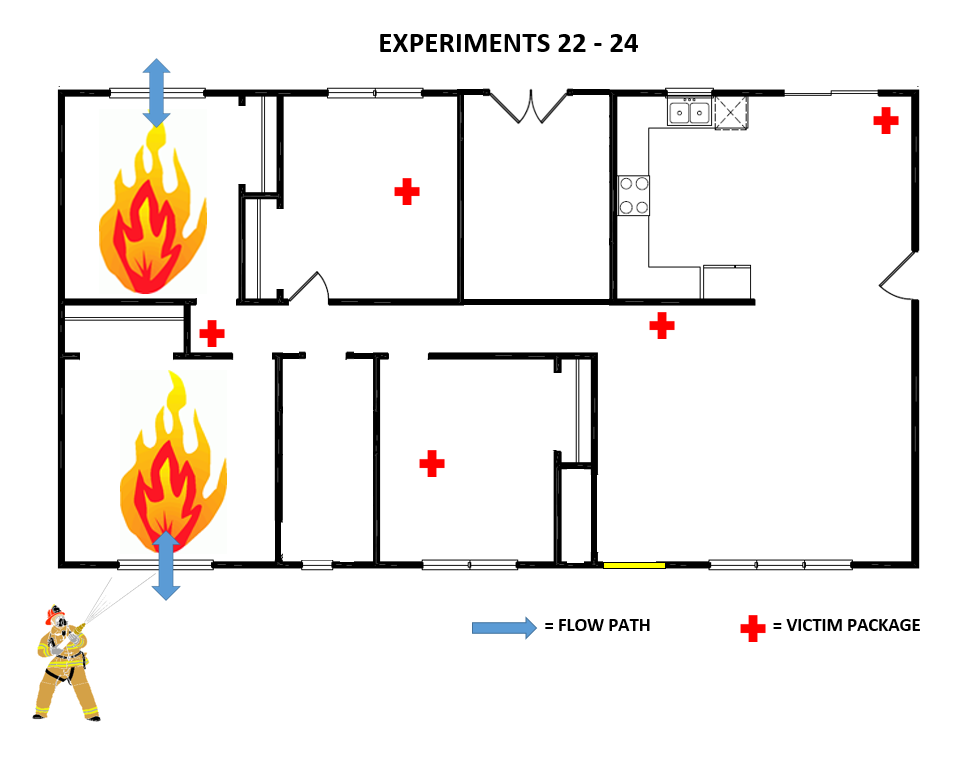
\includegraphics[width=5in]{Figures/General/Exps22through24.png}
	\caption{Configuration for Experiments 22 through 24.}
	\label{fig:ExpConfig22to24}
\end{figure}

\clearpage

\paragraph{Experiment 22} \mbox{}

Experiment 22 is intended to simulate a 2 bedroom fire in a single-story structure with exterior suppression. The fire is ignited in bedroom 1 and bedroom 2. The windows in bedroom 1 and 2 will be open at the start of the experiment. The fire develops and becomes ventilation limited. So at the point of fire attack flow paths exist between the bedroom 1 window and the bedroom1 , between the front door and bedroom 2, between the bedroom 2 window and bedroom 2. Exterior suppression is then initiated using a solid stream pattern with a steep angle and minimal nozzle movement. Interior attack will follow initial knockdown to complete extinguishment. 

Figure~\ref{fig:ExpConfig22to24} shows the configuration of the structure and Table~\ref{Table:Exp22Interventions} shows at what times interventions were performed. 

The results of Experiment 22 can be found in Appendix~\ref{App:Exp22Results}. To view the full experiment video \href{https://youtu.be/gl8rc1Nsl1k}{Click Here}.

\begin{table}[H]
	\centering
	\caption{Experiment 22 Interventions}
	\begin{tabular}{|c|c|} 
		\hline
		Time & Intervention \\ \hline \hline
		00:00 & Ignition - Bedroom \\ \hline
		05:43 & Exterior Suppression BR1 Window Solid Stream \\ \hline
		06:07 & Front Door Open \\ \hline
		06:13 & Attack Team Enters\\ \hline
		06:15 & Burst Suppression \\ \hline 
		06:24 & Hall Suppression \\ \hline
		14:25 & End Experiment\\ \hline
	\end{tabular}
	\label{Table:Exp22Interventions}
\end{table}

\clearpage

\paragraph{Experiment 23} \mbox{}

Experiment 23 is intended to simulate a 2 bedroom fire in a single-story structure with exterior suppression. The fire is ignited simultaneously in bedroom 1 and bedroom 2. As the fire develops, it transitions to a ventilation limited fire. Soon after the fire becomes ventilation limited, exterior suppression will be initiated using a narrow fog stream pattern. Interior attack will be used for extinguishment. 

Figure~\ref{fig:ExpConfig22to24} shows the configuration of the structure and Table~\ref{Table:Exp23Interventions} shows at what times interventions were performed. 

The results of Experiment 23 can be found in Appendix~\ref{App:Exp23Results}. To view the full experiment video \href{https://youtu.be/gl8rc1Nsl1k}{Click Here}.

\begin{table}[H]
	\centering
	\caption{Experiment 23 Interventions}
	\begin{tabular}{|c|c|} 
		\hline
		Time & Intervention \\ \hline \hline
		00:00 & Ignition - Bedroom \\ \hline
		05:26 & Exterior Suppression BR1 Window Narrow Fog Stream \\ \hline
		05:41 & Front Door Open \\ \hline
		05:50 & Attack Team Enters\\ \hline
		06:01 & Hall Suppression \\ \hline 
		12:05 & End Experiment\\ \hline
	\end{tabular}
	\label{Table:Exp23Interventions}
\end{table}

\clearpage

\paragraph{Experiment 24} \mbox{}

Experiment 24 is intended to simulate a 2 bedroom fire in a single-story structure with exterior suppression. The fire is ignited simultaneously in bedroom 1 and bedroom 2. As the fire develops, it transitions to a ventilation limited fire. Soon after the fire becomes ventilation limited, exterior suppression will be initiated using a straight stream pattern followed by content suppression. Interior attack will be used for full extinguishment.

Figure~\ref{fig:ExpConfig22to24} shows the configuration of the structure and Table~\ref{Table:Exp24Interventions} shows at what times interventions were performed. 

The results of Experiment 24 can be found in Appendix~\ref{App:Exp24Results}. To view the full experiment video \href{https://youtu.be/gl8rc1Nsl1k}{Click Here}.

\begin{table}[H]
	\centering
	\caption{Experiment 24 Interventions}
	\begin{tabular}{|c|c|} 
		\hline
		Time & Intervention \\ \hline \hline
		00:00 & Ignition - Bedroom \\ \hline
		05:28 & Exterior Suppression BR1 Window Straight Stream \\ \hline
		05:56 & Exterior Suppression BR2 Window Straight Stream \\ \hline		
		06:16 & Front Door Open \\ \hline
		06:30 & Attack Team Enters\\ \hline
		07:08 & Room Suppression \\ \hline 
		11:55 & End Experiment\\ \hline
	\end{tabular}
	\label{Table:Exp24Interventions}
\end{table}

\clearpage

\chapter{Experiment Analysis}

\section{Repeatability}
The experiments were grouped by the ventilation profile which existed prior to fire department interaction. The three ventilation profiles used were `No Vent', `Single Vent' and `Two Vent'. In the `No Vent', all the openings on the structure were closed until fire department intervention, and the fire was located in Bedroom 1. In the `Single Vent', a single window was open in the fire room (Bedroom 1) until fire department intervention. For the `Two Vent' there were two rooms of fire (Bedroom 1 and Bedroom 2), and the window in each room was open prior to fire department intervention. To compare the effectiveness of the various fire service tactics used in the experiments, it is important to identify if the experiments are comparable across ventilation profiles. 

Each set of experiments in the three ventilation profiles were compared to determine repeatability based on ventilation profile and thus, the applicability of comparing the experiments. The comparison was based on the average temperature measured by the thermocouples in each thermocouple array. The average temperature from each thermocouple array was time-averaged along the period of 60 seconds prior to fire department intervention. In the following sections, the results for each ventilation profile are presented and discussed. 

\subsection{No Vent}
A total of six experiments contained the `No Vent' ventilation profile. The average temperature measured by each thermocouple array averaged across the duration of 60 seconds before fire department intervention is shown in the radar plot presented in Figure~\ref{fig:repeat_No_Vent}. The gray area on the radar plot represents the uncertainty range ($\pm$15~\%) associated with the thermocouple temperature measurement at each measurement location based on the average of the six experiments. With the exception of two instances from Experiment~1, the averaged temperatures are within the gray area and thus, are repeatable for the `No Vent' ventilation profile. 

During Experiment~1, the door to Bedroom 3 was open, while during the other five experiments, the door to Bedroom~3 was closed. The open door accounts for the Experiment~1 temperatures that are outside the uncertainty range: the temperatures at the Victim 3 location and at the Bedroom 3 array location. The temperature measurement locations from all `No Vent' cases can be directly compared with the exception of the Bedroom 3 and Victim 3 locations during Experiment 1, which were outliers and as a result, will not be used in the analysis. 

\begin{figure}[H]
\centering
\includegraphics[width=\textwidth]{../0_Images/Script_Figures/Repeatibility/No_Vent}
\caption{Average Thermocouple Array Temperatures - No Ventilation}
\label{fig:repeat_No_Vent}
\end{figure}

\subsection{Single Vent}
In the `Single Vent' profile, there were 10 experiments. The average temperature for the time period 60 seconds prior to fire department intervention is shown in Figure \ref{fig:repeat_Single_Vent}. The gray area on the radar plot shows the measurement uncertainty for a thermocouple ($\pm$15~\%) at each measurement location based on the average of all experiments. All experiments were within the uncertainty of the measurement and thus, are comparable. All `Single Vent' cases can be directly compared for all temperature measurement locations. 

\begin{figure}[H]
\centering
\includegraphics[width=\textwidth]{../0_Images/Script_Figures/Repeatibility/Single_Vent}
\caption{Average Thermocouple Array Temperatures - Single Vent}
\label{fig:repeat_Single_Vent}
\end{figure}

\subsection{Two Vents}
In the `Two Vent' profile, there were 8 experiments. The average temperature for the time period 60 seconds prior to fire department intervention is shown in Figure \ref{fig:repeat_Two_Vent}. The gray area on the radar plot shows the measurement uncertainty for a thermocouple ($\pm$15~\%) at each measurement location based on the average of all experiments. With the two rooms of fire and two ventilation points, the repeatability decreased slightly from the other two ventilation profiles. Bedroom 2 grew at a faster rate than Bedroom 1, which reduced in some of the Bedroom 1 temperature averages being outside the measurement uncertainty. However, the majority of the other measurement locations were within the measurement uncertainty making all `Two Vent' cases comparable. 

\begin{figure}[H]
\centering
\includegraphics[width=\textwidth]{../0_Images/Script_Figures/Repeatibility/Two_Vent}
\caption{Average Thermocouple Array Temperatures - Two Vent}
\label{fig:repeat_Two_Vent}
\end{figure}

\section{Victim Survivability \& Tenability}
The survivability of a particular fire scenario is difficult to quantify. Factors such as age, gender, and overall health all play a role in how an individual responds to the environment found inside a structure fire. Correlations exist for estimating the threshold from heat energy that would result in a fatality for fifty percent of the general population. Additional correlations exist for irritant and toxic gases however, they focus more on tenability (the dose required for the potential occupant to become incapacitated) and not on survivability (the dose required to cause a fatality). Although it is possible to estimate the survivability based on temperature alone and the tenability based on gas concentrations, no reliable method exists to estimate the combined effects of both temperature and toxic gases. \cite{SFPE:Purser}

Both temperature exposure and toxic gas exposure can be quantified through the use of a Fractional Effective Dose (FED) concept where the FED is equal to the dose received in a given time divided by the effective dose required for a desired endpoint be it incapacitation or death. 

\begin{equation}
	FED = \frac{\text{Dose received at time } t(Ct)}{\text{Effective } Ct \text{ dose to cause incapacitation or death}}
	\label{FED_general}
\end{equation} 

The fractional from carbon monoxide exposure can be calculated as shown in equation \ref{FED_gas} \cite{SFPE:Purser}. The total FED is the integral over the time of exposure $t_1$ to $t_2$ of $3.17 \times  10^{-5}$ multiplied by $CO$, the carbon monoxide concentration in ppm, multiplied by $V$, the volume of air breathed per minute, all divided by $D$ the exposure dose of percent carboxyhemoglobin (COHb) for incapacitation, multiplied by the time step. For this analysis a value of $25~L/min$ was used for $V$, for a victim walking to escape, and a value of 30~\% (COHb) for $D$ for an incapacitating dose.

\begin{equation}
	FED = \int_{t_1}^{t_2}\left(\frac{3.17 \times 10^{-5} \left(CO\right)^{1.036} \left(V\right)}{D}\right) \Delta t
	\label{FED_gas}
\end{equation}

Two methods exist for estimating the effective dose of heat energy received over time, one based on gas temperature and one based on the total heat flux. The method based on total energy flux is the integral from the start of exposure $t_1$ to the end of exposure $t_2$ of the exposure $q$ at time $t$ to the four thirds power, divided by $r$ the heat exposure dose for the endpoint of fatality, $16.7(\sfrac{kW}{m^2})^{\sfrac{4}{3}}$, all multiplied by the exposure time step $\Delta t$ in minutes. \cite{SFPE:Purser}

\begin{equation} \label{TotalFlux_FED}
	FED = \int_{t_1}^{t_2} \left( \frac{q^{4/3}}{r} \right) \Delta t
\end{equation}

The method based on gas temperature as show in equation \ref{GasTemp_FED} is the the integral from the start of exposure $t_1$ to the end of exposure $t_2$ of the gas temperature $T$ in $^{\circ}C$ at time $t$ to the $-9.0403$ power, multiplied by $\num{2e18}$ added to the gas temperature $T$ in $^{\circ}C$ at time $t$ to the $-3.10898$ power multiplied by $\num{e8}$ all multiplied by the time step $\Delta t$ in minutes. \cite{SFPE:Purser}

\begin{equation} \label{GasTemp_FED}
	FED = \int_{t_1}^{t_2} \left( \num{2e18} \times T^{-9.0403} + \num{e8} \times T^{-3.10898} \right) \Delta t
\end{equation}

To determine survivability and tenability a package of sensors were utilized to simulate victims at five different locations within the structure as illustrated in figure \ref{fig:vic_loc}. Victim 1 was located at the end of the hall outside the fire room(s); Victim 2 was located on the bed in Bedroom 3 where the bedroom door was closed; Victim 3 was located on the bed in Bedroom 4 where the bedroom door was open; Victim 4 was located in the Living room near the entrance to the hall; and Victim 5 was located as remote from the fire room(s) as possible in the back right corner of the Dining room. Each location included an array of thermocouples at 1~ft, 3~ft, 5~ft and 7~ft above the floor and schmidt-bloter total heat flux gauge oriented such that the view range of the gauge was directed vertically at 1~ft above the floor. Additionally Victims 1-4 had a gas measurement point analyzing carbon monoxide (CO), carbon dioxide (CO$_{2}$) and oxygen (O$_{2}$) located 1~ft above the floor. Figure XX shows an example of the sensors used. 

\begin{figure}[H]
	\centering
	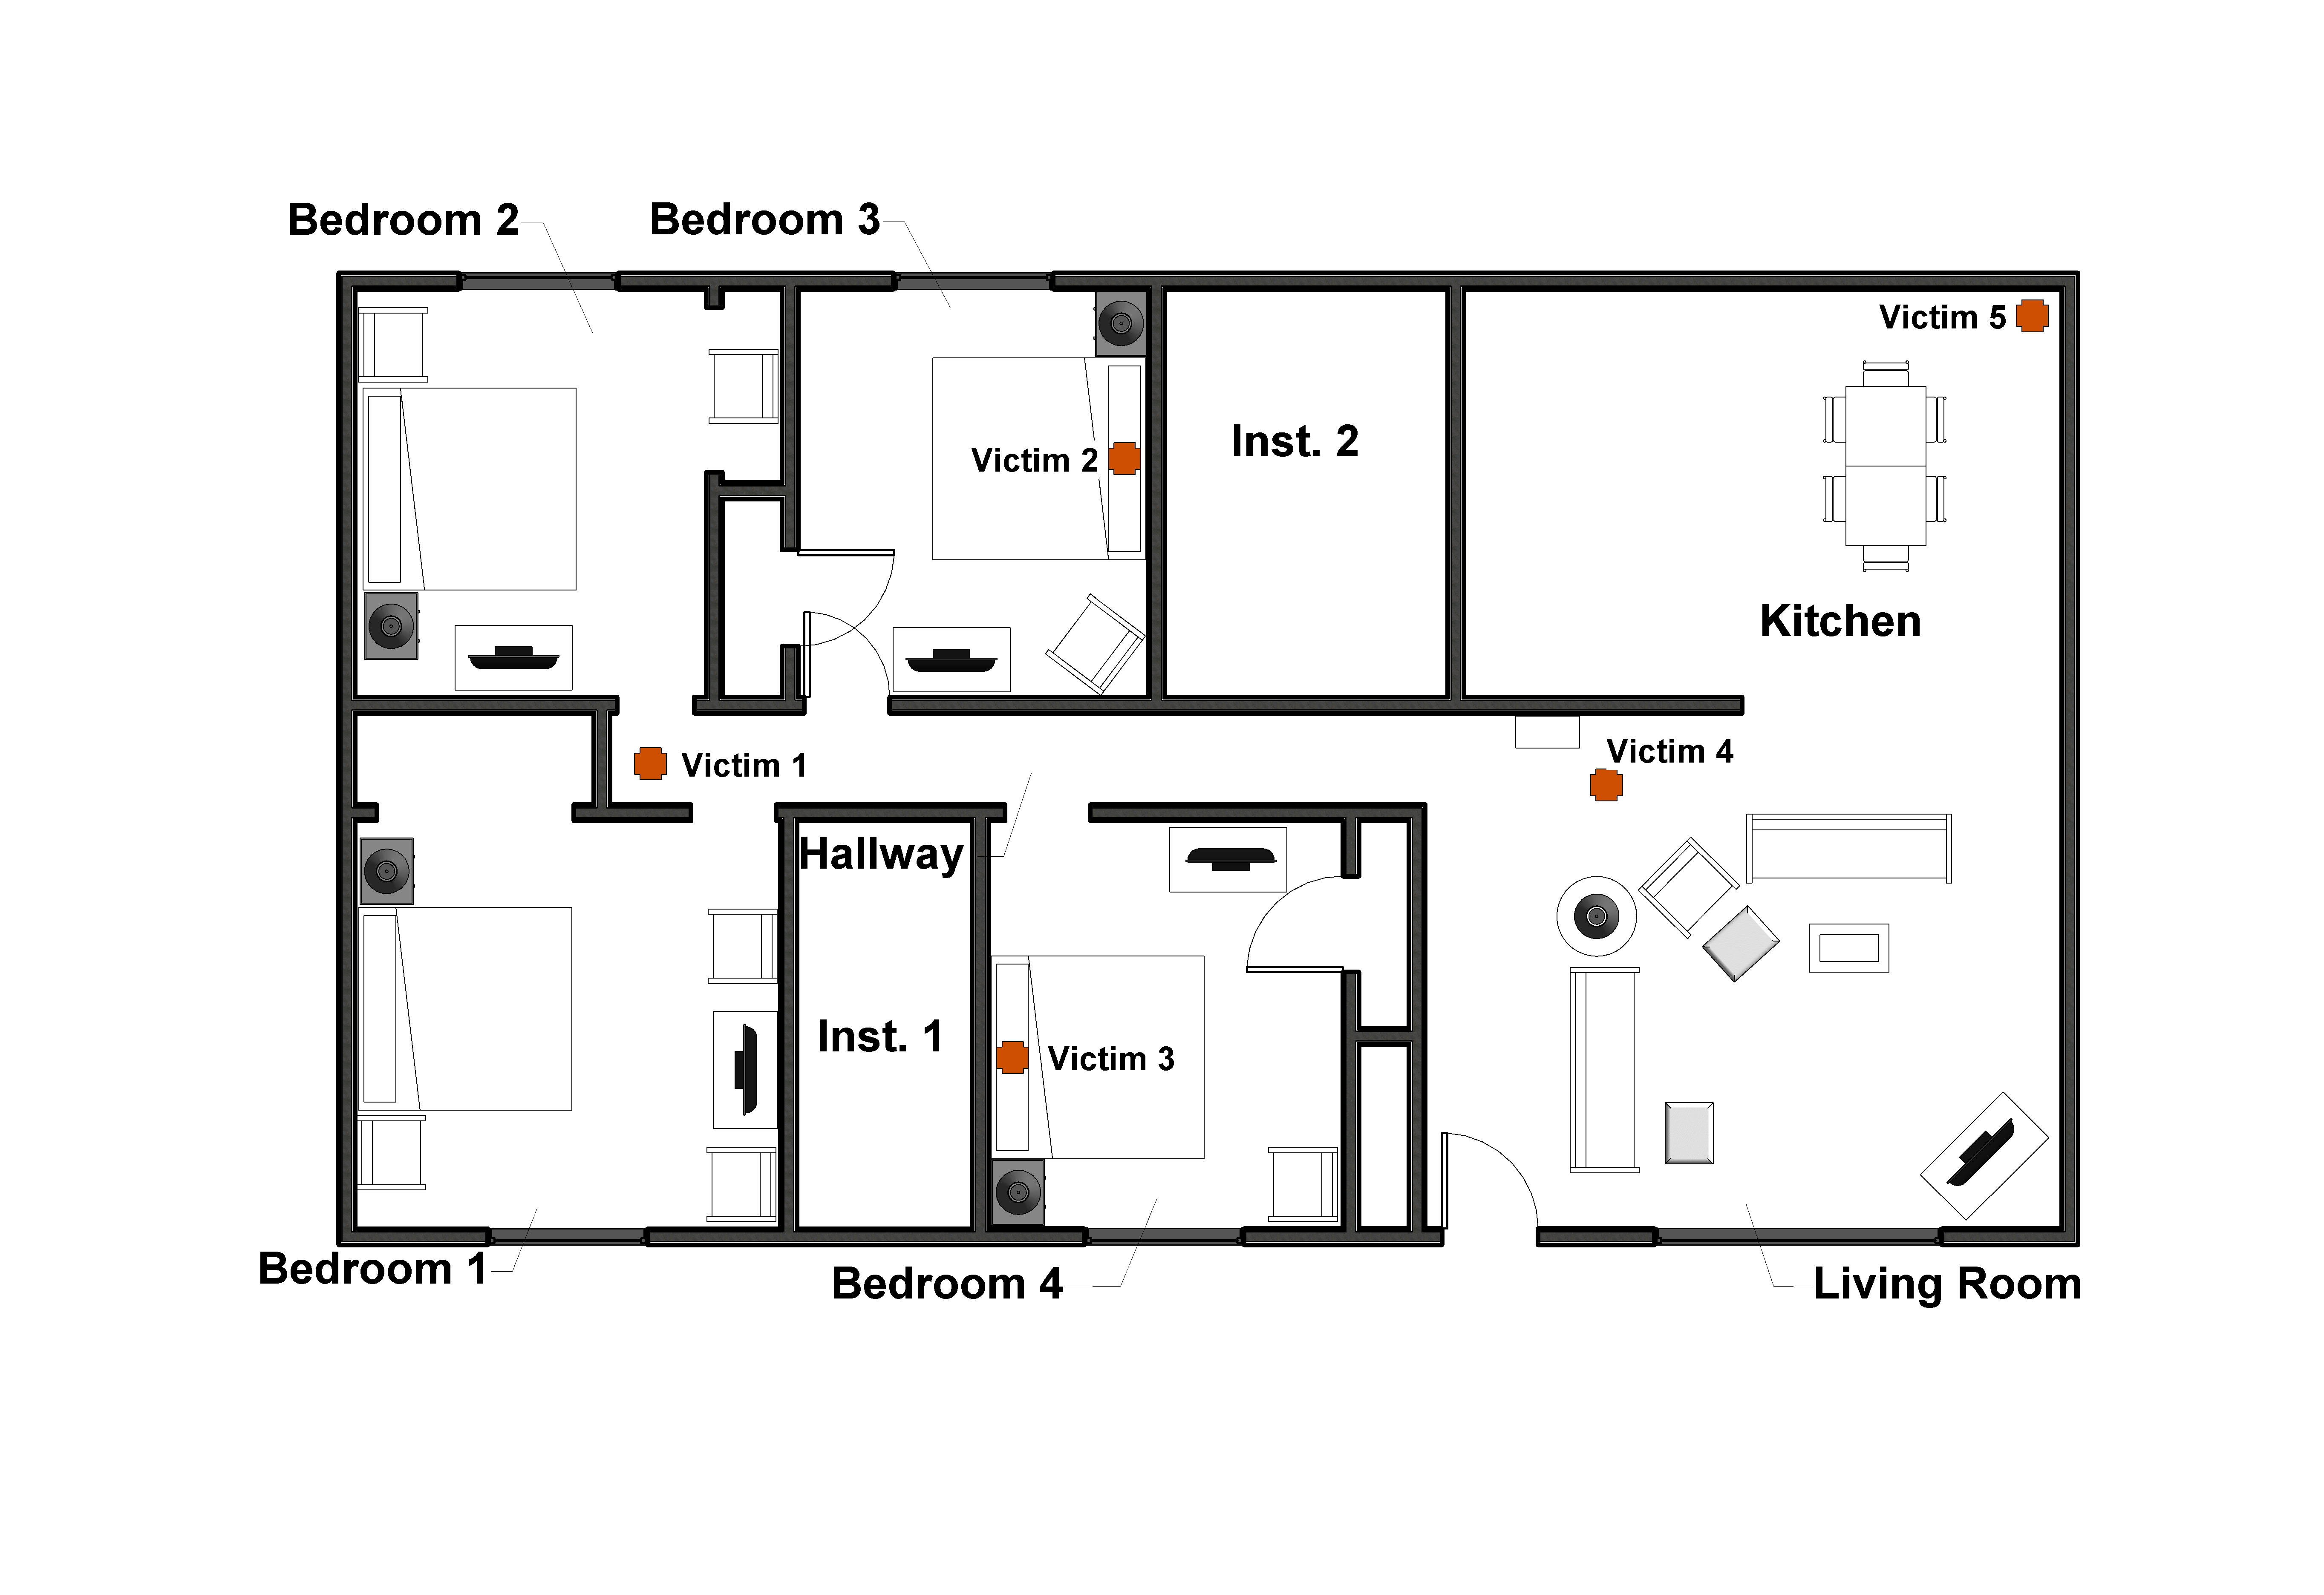
\includegraphics[width=\textwidth]{../0_Images/Victim_Locations}
	\caption{Victim Locations}
	\label{fig:vic_loc}
\end{figure}

The CO, CO$_{2}$, and O$_{2}$ values from the gas analyzers were utilized in equation \ref{FED_gas} to determine the fraction of dose required for untenability. A value of 1 represents untenable and a value of 3 represents a potentially fatal dose. The gas temperature recorded via the 1~ft thermocouple was used in equation \ref{GasTemp_FED} to determine the fraction of a fatal dose received via convective heat transfer, where a value of 1 is equivalent to a fatal dose in 50~\% of the population. The total heat flux recorded at the  schmidt-bolter heat flux gauge was used in equation \ref{TotalFlux_FED} to determine the fraction of a fatal does received via both convective and radiative heat transfer, where a value of 1 is equivalent to a fatal dose in 50~\% of the population, .  

This section will analyze the experiments conducted for survivability of the five victim locations shown in  based on temperature an tenability based on gas concentrations in the period prior to fire department arrival and then as they relate to the possible fire suppression tactics. 

\subsection{Prior Fire Department Arrival}
To examine the potential survivability and tenability prior to fire department intervention the experiments were grouped by the available ventilation. The average fractional effective dose over time was calculated for each victim location along with the value of one standard deviation. 

\subsubsection{No Ventilation}

Figure \ref{fig:Vent_Profile-No_Vent} represents the no ventilation configuration where all exterior windows/doors were closed. The fire was located in bedroom 1 and fire department intervention occurred at 6~minutes and 58~seconds, after the fire reached a ventilation limited state . 

\begin{figure}[H]
	\centering
	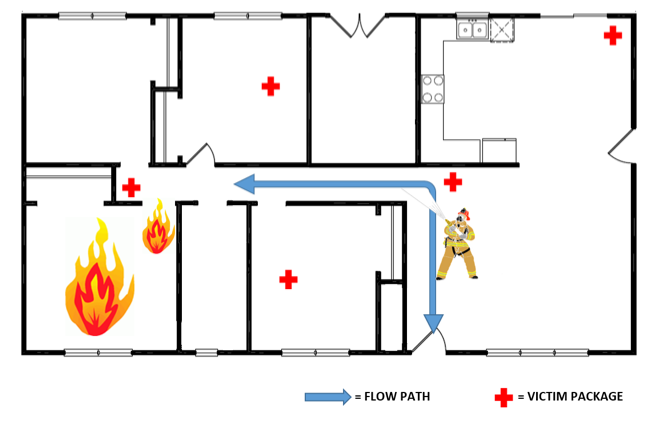
\includegraphics[width=.65\textwidth]{../0_Images/Ventilation_Configurations/No_Vent.png}
	\caption{Ventilation Configuration - No Ventilation (Experiments 1-6)}
	\label{fig:Vent_Profile-No_Vent}
\end{figure}

 Figure \ref{fig:FED_NoVent} illistrates the average fractional effective dose over time at each of the victim locations relative to toxic gases, convective heat transfer and both radative and convective heat transfer. The shaded areas represent +/- one standard deviation from the average value with the shaded color corresponding to the victim location. 

\begin{figure}[H]
	\centering
	\includegraphics[width=.45\textwidth]{../0_Images/Script_Figures/FED/FED_Avg_Gas/No_Vent}
	\includegraphics[width=.45\textwidth]{../0_Images/Script_Figures/FED/FED_Avg_Temp_Conv/No_Vent} 
	\includegraphics[width=.45\textwidth]{../0_Images/Script_Figures/FED/FED_Avg_Temp_FLux/No_Vent}
	\caption[No Vent Fractional Effective Dose]{No Ventilation Fractional Effective Dose Prior to Fire Department Arrival. Left is based on gas concentration, center is based on convective heat transfer and right is based on both convective and radiative transfer}
	\label{fig:FED_NoVent}
\end{figure}

With regards to the toxic gases both survivability and tenability are related to the elevation in the space, along with the proximity to the fire. Victim 3 located on the bed in the open bedroom, once the smoke layer reached the victim the FED increased rapidly, exceeding an FED of 3 between 5~min 30~sec and 6~min 30~sec. The smoke took significantly longer to reach Victims located at the floor level, resulting in a lower FED at the time of fire department arrival. Victim 4 being more remote to the fire shows a higher FED than victim 1 near the fire as the flow path carried the smoke to the floor level in the remote locations first as the ambient air was drawn back to the fire keeping Victim 1 in the ambient air longer. 

The survivability in terms of heat energy is driven more by the radiative energy transfer than the convective. The FED based strictly on convective transfer shows almost no increase prior to fire department arrival. When both radiative and convective heat transfer are examined, all of the victim locations are below the threshold for fatality in 50~\% of the population. Victim 1, was shown to have the highest FED value due to the proximity of the fire followed by the victim 3 location which is within the hot gas layer. For the remainder of the locations FED was driven by the proximity to the fire where victim 4 was closer than victim 5. The effectiveness of a closed bedroom door is illustrated by the victim 2 location value being the lowest. 

\subsubsection{Single Window Vent}

Figure \ref{fig:Vent_Profile-Single_Vent} represents the ventilation configuration where all exterior windows/doors were closed with the exception of the bedroom 1 window. The fire was located in bedroom 1 and fire department intervention occurred  at 5~minutes and 26~seconds, after the fire reached a flashover. 

\begin{figure}[H]
	\centering
	\includegraphics[width=.65\textwidth]{../0_Images/Ventilation_Configurations/Single_Vent.png}
	\caption{Ventilation Configuration - Single Window Vent (Experiments 7-12 \& 18-21)}
	\label{fig:Vent_Profile-Single_Vent}
\end{figure}

Figure \ref{fig:FED_SingleVent} illustrates the average fractional effective dose over time at each of the victim locations relative to toxic gases, convective heat transfer and both radative and convective heat transfer. The shaded areas represent +/- one standard deviation from the average value with the shaded color corresponding to the victim location. 

\begin{figure}[H]
	\centering
	\includegraphics[width=.45\textwidth]{../0_Images/Script_Figures/FED/FED_Avg_Gas/Single_Vent}
	\includegraphics[width=.45\textwidth]{../0_Images/Script_Figures/FED/FED_Avg_Temp_Conv/Single_Vent} 
	\includegraphics[width=.45\textwidth]{../0_Images/Script_Figures/FED/FED_Avg_Temp_FLux/Single_Vent}
	\caption[Single Window Vent Fractional Effective Dose]{Single Window Vent Fractional Effective Dose Prior to Fire Department Arrival. Left is based on gas concentration, center is based on convective heat transfer and right is based on both convective and radiative transfer}
	\label{fig:FED_SingleVent}
\end{figure}

The fire department intervention was preformed in just over 5~minutes limiting the time available for the gases too reach the victim locations. This resulted in an FED from toxic gases at the time of intervention which indicates a tenable and survivable space at each location. The FED at the victim 3 location began to increase just before intervention, indicating the time to untenability and fatality is approaching. 

The survivability in terms of heat energy was also less due to the decreased duration of exposure. It was driven more by the radiative energy transfer than the convective. The FED based strictly on convective transfer shows almost no increase prior to fire department intervention. When both radiative and convective heat transfer are examined, all of the victim locations are below the threshold for fatality in 50~\% of the population. The victim 1 location, had the highest FED value due to the proximity of the fire however the other four locations show almost no FED. 

\subsubsection{Two Window Vents, Two Rooms of Fire}

Figure \ref{fig:Vent_Profile-Two_Vent} represents the ventilation configuration where all exterior windows/doors were closed with the exception of the bedroom 1 and bedroom 2 windows. The fire was located in both bedroom 1 and bedroom 2. Fire department intervention occurred at 5~minutes and 24~seconds, after the fire reached a flashover. 

\begin{figure}[H]
	\centering
	\includegraphics[width=.65\textwidth]{../0_Images/Ventilation_Configurations/Two_Vent.png}
	\caption{Ventilation Configuration - Single Window Vent (Experiments 13-17 \& 22-24)}
	\label{fig:Vent_Profile-Two_Vent}
\end{figure}

Figure \ref{fig:FED_TwoVent} illustrates the average fractional effective dose over time at each of the victim locations relative to toxic gases, convective heat transfer and both radiative and convective heat transfer. The shaded areas represent +/- one standard deviation from the average value with the shaded color corresponding to the victim location. 

\begin{figure}[H]
	\centering
	\includegraphics[width=.45\textwidth]{../0_Images/Script_Figures/FED/FED_Avg_Gas/Two_Vent}
	\includegraphics[width=.45\textwidth]{../0_Images/Script_Figures/FED/FED_Avg_Temp_Conv/Two_Vent} 
	\includegraphics[width=.45\textwidth]{../0_Images/Script_Figures/FED/FED_Avg_Temp_FLux/Two_Vent}
	\caption[Two Window Vent Fractional Effective Dose]{Two Window Vent Fractional Effective Dose Prior to Fire Department Arrival. Left is based on gas concentration, center is based on convective heat transfer and right is based on both convective and radiative transfer}
	\label{fig:FED_TwoVent}
\end{figure}

The tenability and survivability based on toxic gas was again driven by the elevation in the space. With two rooms of fire and two ventilation openings the victim 3 location on the bed in the open bedroom exceeded a FED of 3 in just under 5~minutes. The smoke took longer to reach the 1~ft level, thus all other victim locations show almost no increase in FED at fire department intervention.

The survivability in terms of heat energy was driven more by the radiative energy transfer than the convective. The FED based strictly on convective transfer shows a fatal dose of energy in just over three minutes at the victim 1 location and no increase prior to fire department intervention at the remainder of the 4 victim locations. When both radiative and convective heat transfer are examined, the victim 1 location receives a fatal dose in just under 3~minutes 30~seconds. After that point the FED is driven by the elevation in the space with locations in the hot gas layer receiving more FED than those at the floor. After the 5~minute mark all victim locations are receiving a thermal FED with the exception of the victim 2 location behind the closed door.  

\subsubsection{FED Ventilation Comparison}
When comparing the FED for the three ventilation cases it is important to consider both the size of the fire and the timing. Although it may appear initially the case with no ventilation resulted in higher FED values, however that is because it involved a greater duration. Three experiments were conducted with delayed water application to determine evaluate the effect of delayed water. 

A comparison of the FED for each victim location is shown in Figure \ref{fig:FED_Base} where a FED of 1.0 for the thermal values of convective and total flux represents the lethal concentration for 50~\% of the population (LC50) and  a FED of 1.0 for the toxic gases represents a untenable condition where occupants would not be able to self rescue. 

Experiment 1 had no ventilation, see figure \ref{fig:FED_NoVent} for the ventilation profile. The front door was opened at 8~minutes 17~seconds. Experiment 12 had the bedroom 2 window open, see figure \ref{fig:FED_SingleVent} for the the ventilation profile. The front door was opened at 5~minutes and 57~seconds. Experiment 17 had two rooms a fire in bedroom 1 and bedroom 2 with both bedroom windows open, see figure \ref{fig:FED_TwoVent} for the ventilation profile. The front door was opened at 5~minutes and 27~seconds. 

The 'Total Flux' value refers to the FED calculated from equation \ref{TotalFlux_FED}, the 'Convective' value refers to the FED calculated from equation \ref{GasTemp_FED} and the 'Toxic Gas' value refers to the FED calculated from equation \ref{GasTemp_FED}.

\begin{figure}[H]
	\centering
	\includegraphics[width=0.4\textwidth]{../0_Images/Script_Figures/FED/FED_Base/Victim_1}
	\includegraphics[width=0.4\textwidth]{../0_Images/Script_Figures/FED/FED_Base/Victim_2}
	\includegraphics[width=0.4\textwidth]{../0_Images/Script_Figures/FED/FED_Base/Victim_3}
	\includegraphics[width=0.4\textwidth]{../0_Images/Script_Figures/FED/FED_Base/Victim_4}
	\includegraphics[width=0.4\textwidth]{../0_Images/Script_Figures/FED/FED_Base/Victim_5}
	\caption[Ventilation Comparison - FED]{Ventilation Comparison - Fractional Effective Dose. Upper left is victim 1, upper right is victim 2. Middle left is victim 3, middle right is victim 4. Lower center is victim 5. A FED of 1.0 for thermal values is the LC50 for thermal exposure. A FED of 1.0 for toxic gases represents untenable conditions.}
	\label{fig:FED_Base}
\end{figure}

The victim location 1 shows that the in the two vent case the thermal hazard is the most significant, for the no vent case it is the toxic gases. In the victim 2 case, being behind the closed door provides a survivable and tenable atmosphere. At the victim 3 location the driving hazard is the toxic gases which accumulate first for the two room fire, followed by the no vent case and lastly by th event case. In all instances the toxic gases exceed a FED of 3.0 by just over 8~minutes. The Victim 4 location is far enough from the fire thermal hazards are not as significant however toxic gases are a hazard. Once the door gets opened at 5~minutes and 27~seconds in the two vent case, and 8~minutes and 17~seconds in the no vent case, the ambient air slows the increase of FED. No toxic gas values were available at victim 5 however the values were below the LC50 for thermal hazards. 

\clearpage

\subsection{Effect of Fire Department Intervention}
This section looks at the difference between fire department intervention and delayed intervention quantifying tenability of the four locations. This will be an average value of all interventions compared to the value with delayed intervention. \\
\textbf{\hl{Compare 1 vs. 2-6 (No Vent)}} \\
\textbf{\hl{Compare 12 vs. 7-11 \& 18-21 \& 27 (Single Vent)}} \\
\textbf{\hl{Compare 17 vs. 13-16 \& 22-24 (Two Vent)}} \\

\subsection{Interior vs. Exterior}
This section looks at the effect of different fire department tactics on tenability. Specifically the difference in FED from onset of intervention to onset plus longest intervention time. \\
\textbf{\hl{Compare 7-11 vs. 18-21 \& 27 (Single Vent)}} \\
\textbf{\hl{Compare 13-16 vs. 22-24 (Two Vent)}} \\

\section{Effect of Ventilation Profile on Knock Back Capability}
In the following section, knock back times are compared between experiments from five different groups that were formed based on fire attack method. Three of the sets involved an interior fire attack method, and two sets involved an exterior fire attack method. This section compares the temperature data from the experiments in each set to determine how ventilation profile and fire size affect the ability of the different attack methods to knock back the fire. 

\subsection{Interior}
The differentiating factor between the three sets of interior fire attack experiments is the type of method used to extinguish the fire, and the differentiating factor between the experiments within each set is the ventilation profile and fire size. 

The first set of experiments contains experiments that used the ``flow and move'' attack method with a solid stream from a smooth bore nozzle. The group is composed of Experiments~2, 7, and 13, which contained the `No Vent', `Single Vent', and `Two Vent' ventilation profiles, respectively.

\begin{figure}[H]
	\centering
	\includegraphics[width=0.48\textwidth]{../0_Images/Script_Figures/Knock_Back/Experiment_2_Bedroom_1_Temps}
	\includegraphics[width=0.48\textwidth]{../0_Images/Script_Figures/Knock_Back/Experiment_7_Bedroom_1_Temps}
	\includegraphics[width=0.48\textwidth]{../0_Images/Script_Figures/Knock_Back/Experiment_13_Bedroom_1_Temps}
	\caption[]{Experiments 2 (top left), 7 (top right), and 13 (bottom) Bedroom 1 temperatures around time of suppression}
	\label{fig:knockback_int_1}
\end{figure}
\clearpage

The second set of experiments contains experiments that used the ``shutdown and move'' attack method with a solid stream from a smooth bore nozzle. The group is composed of Experiments~6, 8, and 14, which contained the `No Vent', `Single Vent', and `Two Vent' ventilation profiles, respectively.

\begin{figure}[!ht]
	\centering
	\includegraphics[width=0.48\textwidth]{../0_Images/Script_Figures/Knock_Back/Experiment_6_Bedroom_1_Temps}
	\includegraphics[width=0.48\textwidth]{../0_Images/Script_Figures/Knock_Back/Experiment_8_Bedroom_1_Temps}
	\includegraphics[width=0.48\textwidth]{../0_Images/Script_Figures/Knock_Back/Experiment_14_Bedroom_1_Temps}
	\caption[]{Experiments 6 (top left), 8 (top right), and 14 (bottom) Bedroom 1 temperatures around time of suppression}
	\label{fig:knockback_int_2}
\end{figure}
\clearpage

The third set of experiments contains experiments that used the ``flow and move'' attack method with a narrow fog stream from a combination nozzle. The group is composed of Experiments~11 and 16, which contained the `Single Vent' and `Two Vent' ventilation profiles, respectively.

\begin{figure}[H]
	\centering
	\includegraphics[width=0.48\textwidth]{../0_Images/Script_Figures/Knock_Back/Experiment_11_Bedroom_1_Temps}
	\includegraphics[width=0.48\textwidth]{../0_Images/Script_Figures/Knock_Back/Experiment_16_Bedroom_1_Temps}
	\caption[]{Experiments 11 (left) and 16 (right) Bedroom 1 temperatures around time of suppression}
	\label{fig:knockback_int_3}
\end{figure}
\clearpage

\subsection{Exterior}
\textbf{\hl{Compare 18,20, (just initial hit) vs. 22,24 (just bedroom 1)}}
\begin{figure}[H]
	\centering
	\includegraphics[width=0.48\textwidth]{../0_Images/Script_Figures/Knock_Back/Experiment_18_Bedroom_1_Temps}
	\includegraphics[width=0.48\textwidth]{../0_Images/Script_Figures/Knock_Back/Experiment_20_Bedroom_1_Temps}
	\includegraphics[width=0.48\textwidth]{../0_Images/Script_Figures/Knock_Back/Experiment_22_Bedroom_1_Temps}
	\includegraphics[width=0.48\textwidth]{../0_Images/Script_Figures/Knock_Back/Experiment_24_Bedroom_1_Temps}
	\caption[]{Experiments 18 (top left), 20 (top right), 22 (bottom left), and 24 (bottom right) Bedroom 1 temperatures around time of initial suppression.}
	\label{fig:knockback_ext_1}
\end{figure}
\clearpage

\textbf{\hl{Compare 22 (BD1 and interior) vs. 24 (BD1, BD2, and Interior)}}
\begin{figure}[H]
	\centering
	\includegraphics[width=0.48\textwidth]{../0_Images/Script_Figures/Knock_Back/Experiment_22_Bedroom_1_Temps_full}
	\includegraphics[width=0.48\textwidth]{../0_Images/Script_Figures/Knock_Back/Experiment_22_Bedroom_2_Temps_full}
	\includegraphics[width=0.48\textwidth]{../0_Images/Script_Figures/Knock_Back/Experiment_24_Bedroom_1_Temps_full}
	\includegraphics[width=0.48\textwidth]{../0_Images/Script_Figures/Knock_Back/Experiment_24_Bedroom_2_Temps_full}
	\caption[]{Experiments 22 (top) and 24 (bottom) Bedroom 1 temperatures (left column) and Bedroom 2 temperatures (right column) during suppression events.}
	\label{fig:knockback_ext_2}
\end{figure}
\clearpage

\begin{figure}[H]
	\centering
	\includegraphics[width=0.48\textwidth]{../0_Images/Script_Figures/Knock_Back/Experiment_22_End_Hall_Temps_full}
	\includegraphics[width=0.48\textwidth]{../0_Images/Script_Figures/Knock_Back/Experiment_22_Bedroom_4_Temps_full}
	\includegraphics[width=0.48\textwidth]{../0_Images/Script_Figures/Knock_Back/Experiment_24_End_Hall_Temps_full}
	\includegraphics[width=0.48\textwidth]{../0_Images/Script_Figures/Knock_Back/Experiment_24_Bedroom_4_Temps_full}
	\caption[]{Experiments 22 (top) and 24 (bottom) end of the hall temperatures (left column) and Bedroom 4 temperatures (right column) during suppression events.}
	\label{fig:knockback_ext_3}
\end{figure}
\clearpage

\section{Ability to Influence the Flow of Products of Combustion}
This test series included specific instrumentation to evaluate the ability of hose streams to move products of combustion in residential structure fires. Instrumentation was installed at the window when exhaust was provided, at the door to the fire room, and at the start of the hallways to evaluate the flows during the different suppression tactics. Additionally pressure sensors were located at the front door and in bedroom 2 to evaluate the pressure changes when water was flowing. 

\subsection{Interior}
The velocity probes at the start of the hallway and the window to the fire room show that flowing water down the hallway has the ability to stop the flow of smoke out of the hallway and create a unidirectional vent at the window.

\subsubsection{Impact of Advancement Type on Pressure Created}

\subsubsection{Impact of Ventilation Profile on Pressure Created}
\textbf{\hl{Compare 2, 7 , 13 (Flow and move SB)}} \\
\textbf{\hl{Compare 6, 8 , 14 (Shutdown and move SB)}} \\
\textbf{\hl{Compare 11, 16 (flow and move Fog)}} \\

\subsection{Exterior}
\textbf{\hl{Compare 20(door closed) vs 21 (front door open)}} \\
\textbf{\hl{Compare 19(one room fire) vs 23 (two rooms fire)}} \\

\section{Impact of ``Whip'' on Regrowth}
\textbf{\hl{compare 18 (no whip) vs 20(whip) (front door closed)}} \\

\section{Impact of Door Control}
\textbf{\hl{Compare 3 (door control) with 6 (no control)}} \\
\textbf{\hl{Compare 14 (no control) with 15 (door control)}} \\

\normalfont

\section{Flowing While Moving vs. Shutting Down to Move}
There were two methods of approach to the fire. The first titled `flow and move' involved flowing the hose line while moving down the hallway towards the fire room. The second titled `shutdown and move' involved flowing the nozzle from a fixed position, shutting it down, moving up to the next position, flowing again, shutting it down and moving to the next position until the crew reached the fire room. This section will compare these two tactics as they relate to temperatures in the approach path, temperatures in the fire room, and gas velocities in the hallway for the three ventilation cases tested. 

\subsection{Approach Temperatures}

The single room fires with no ventilation as illustrated in Figure \ref{fig:Vent_Profile-No_Vent} were interior attacks with no ventilation opposite. Figure \ref{fig:Flow_vs_Shut_Single_No_Vent} shows the comparison between the flow and move tactic and shutdown and move tactic. With no ventilation provided opposite the attack crew, the shutdown and move tactic results in temperatures rebounding in the upper level of the hallway when the line is shutdown as the attack crew makes their way down the hallway. This is not seen in the flow and move tactic as the hose stream is continuously cooling as the crew makes their way down the hallway. 

\begin{figure}[H]
\centering
\includegraphics[width=0.495\textwidth]{../0_Images/Script_Figures/Experiment_Analysis/Flow_vs_Shutdown/Experiment_2/End_Hall}
\includegraphics[width=0.495\textwidth]{../0_Images/Script_Figures/Experiment_Analysis/Flow_vs_Shutdown/Experiment_6/End_Hall}
\caption[Single Room - No Vent - Flow \& Move vs. Shutdown \& Move - Hall Temperature]{End of Hallway Temperatures (3TC) for the two attack methods used in the single room of fire with no ventilation. The blue shaded areas represent water flow from the hose stream. The right shows a flow and move tactic from Experiment 2 and the left shows the shutdown and move tactic Experiment 6.}
\label{fig:Flow_vs_Shut_Single_No_Vent}
\end{figure}

Ventilation, provided opposite the attack crew, has little impact on the flow and move vs. shutdown and move tactics as seen in Figure \ref{fig:Flow_vs_Shut_Single_Vent}for the single room fire and Figure \ref{fig:Flow_vs_Shut_Two_Vent} for the two rooms of fire. The same temperature rebounding occurs in the shutdown and move case, it is again not seen in the flow and move case. 

\begin{figure}[H]
\centering
\includegraphics[width=0.495\textwidth]{../0_Images/Script_Figures/Experiment_Analysis/Flow_vs_Shutdown/Experiment_7/End_Hall}
\includegraphics[width=0.495\textwidth]{../0_Images/Script_Figures/Experiment_Analysis/Flow_vs_Shutdown/Experiment_8/End_Hall}
\caption[Single Room - Window Vent Opposite - Flow \& Move vs. Shutdown \& Move - Temperature]{End of Hallway Temperatures (3TC) for the two attack methods used in the single room of fire with ventilation opposite the attack crew. The blue shaded areas represent water flow from the hose stream. The right shows a flow and move tactic from Experiment 7 and the left shows the shutdown and move tactic Experiment 8.}
\label{fig:Flow_vs_Shut_Single_Vent}
\end{figure} 

\begin{figure}[H]
\centering
\includegraphics[width=0.495\textwidth]{../0_Images/Script_Figures/Experiment_Analysis/Flow_vs_Shutdown/Experiment_13/End_Hall}
\includegraphics[width=0.495\textwidth]{../0_Images/Script_Figures/Experiment_Analysis/Flow_vs_Shutdown/Experiment_14/End_Hall}
\caption[Two Room - Two Vents Opposite - Flow \& Move vs. Shutdown \& Move - Temperature]{End of Hallway Temperatures (3TC) for the two attack methods used in the two rooms of fire with two windows of ventilation opposite the attack crew. The blue shaded areas represent water flow from the hose stream. The right shows a flow and move tactic from Experiment 13 and the left shows the shutdown and move tactic from Experiment 14.}
\label{fig:Flow_vs_Shut_Two_Vent}
\end{figure}

\subsection{Fire Room Temperatures}
The ultimate goal of any method of fire attack is to extinguish the fire in the fire compartment. When comparing the flow and move tactic and shutdown and move tactics it is important to note the effect on the fire room during approach. Figure \ref{fig:Flow_vs_Shut_Single_No_Vent_Fire_Temp} shows the two tactics and their effect on the fire room temperatures. In the flow and move case, initially the water has no impact on the fire compartment as it is not physically possible for water to enter the compartment from the position the crew began to flow water. As the crew advanced down the hallway, water begins to enter the compartment and effect the fire. It is not until the crew reaches the compartment that greatest impact occurs. For the shutdown and move case it is more pronounced as neither the first nor second position in the hall resulted in temperature reduction in the fire room. It was not until the crew was at the end of the hall flowing into the fire room that the water had an impact on temperatures. 

\begin{figure}[H]
\centering
\includegraphics[width=0.495\textwidth]{../0_Images/Script_Figures/Experiment_Analysis/Flow_vs_Shutdown/Experiment_2/Bedroom_1}
\includegraphics[width=0.495\textwidth]{../0_Images/Script_Figures/Experiment_Analysis/Flow_vs_Shutdown/Experiment_6/Bedroom_1}
\caption[Single Room - No Vent - Flow \& Move vs. Shutdown \& Move - Bedroom 1 Temperature]{Fire Room (Bedroom 1) Temperatures (1TC) for the two attack methods used in the single room of fire with no ventilation. The blue shaded areas represent water flow from the hose stream. The right shows a flow and move tactic from Experiment 2 and the left shows the shutdown and move tactic Experiment 6.}
\label{fig:Flow_vs_Shut_Single_No_Vent_Fire_Temp}
\end{figure}

Providing a vent opposite the attack crew does as seen in Figure \ref{fig:Flow_vs_Shut_Single_Vent_Fire_Temp} does not change the effect of the tactics on the fire room. The water being directed down the hall in both the flow and move and shutdown and move cases cannot impact the fire room from the entrance to the hallway. It is not until the crew makes it to the midpoint of the hallway that water can enter the room and begin to have an effect. It isn't until the crew reaches the fire room and is able to direct the stream into the compartment that the temperatures drop significantly.  

\begin{figure}[H]
\centering
\includegraphics[width=0.495\textwidth]{../0_Images/Script_Figures/Experiment_Analysis/Flow_vs_Shutdown/Experiment_9/Bedroom_1}
\includegraphics[width=0.495\textwidth]{../0_Images/Script_Figures/Experiment_Analysis/Flow_vs_Shutdown/Experiment_10/Bedroom_1}
\caption[Single Room - Window Vent Opposite - Flow \& Move vs. Shutdown \& Move - Bedroom 1 Temperature]{Fire Room (Bedroom 1) Temperatures (1TC) for the two attack methods used in the single room of fire with a window vent opposite the attack crew. The blue shaded areas represent water flow from the hose stream. The right shows a flow and move tactic from Experiment 9 and the left shows the shutdown and move tactic Experiment 10.}
\label{fig:Flow_vs_Shut_Single_Vent_Fire_Temp}
\end{figure}

With an additional room of fire in the two rooms of fire with two window vents opposite as seen in Figure \ref{fig:Flow_vs_Shut_Two_Vent_Fire_Temp} the additional energy being released from the fire results in more difficulty in cooling the fire compartment.  

\begin{figure}[H]
\centering
\includegraphics[width=0.495\textwidth]{../0_Images/Script_Figures/Experiment_Analysis/Flow_vs_Shutdown/Experiment_13/Bedroom_1}
\includegraphics[width=0.495\textwidth]{../0_Images/Script_Figures/Experiment_Analysis/Flow_vs_Shutdown/Experiment_14/Bedroom_1}
\caption[Two Room - Two Vents Opposite - Flow \& Move vs. Shutdown \& Move - Bedroom 1 Temperature]{Fire Room (Bedroom 1) Temperatures (1TC) for the two attack methods used in the single room of fire with a window vent opposite the attack crew. The blue shaded areas represent water flow from the hose stream. The right shows a flow and move tactic from Experiment 13 and the left shows the shutdown and move tactic Experiment 14.}
\label{fig:Flow_vs_Shut_Two_Vent_Fire_Temp}
\end{figure}

% \begin{figure}[H]
% \centering
% \includegraphics[width=0.495\textwidth]{}
% \includegraphics[width=0.495\textwidth]{}
% \caption{}
% \label{}
% \end{figure}

\subsection{Gas Velocity}
Examining the air movement at the start of the hallway for the two cases illustrates the ability of the hose stream to move products of combustion away from the nozzle crew and draw air in behind them as the make their way down the hallway. For the case with no ventilation opposite the advancing attack crew, Figure \ref{fig:Flow_vs_Shut_Single_No_Vent_Velocity} shows that the gas velocity at the top of the hallway goes from approximately 5~m/s out toward the front door to roughly 0~m/s on the initial flow, and the values of the lower gas velocity probes go from flowing down the hallway toward the fire to 0~m/s as well stopping flow. 

As the crew advances down the hallway in the flow and move tactic, all velocities maintain a flow near 0~m/s until the nozzle is shut down where. The flow at the top of the opening returns to about 1~m/s as the products of combustion seek the low pressure at the front door.  With the shutdown and move case, as the crew shutdown the nozzle to move the gas velocities return in between flows to values of about 2.5~m/s or half the initial velocity. Once the crew reaches the fire room and conducts the last flow, the gas velocity at the top of the door returns to 1~m/s as the combustion products seek the low pressure much like the flow and move case.

\begin{figure}[H]
\centering
\includegraphics[width=0.495\textwidth]{../0_Images/Script_Figures/Experiment_Analysis/Flow_vs_Shutdown/Experiment_2/Start_Hall_Flow}
\includegraphics[width=0.495\textwidth]{../0_Images/Script_Figures/Experiment_Analysis/Flow_vs_Shutdown/Experiment_6/Start_Hall_Flow}
\caption[Single Room - No Vent - Flow \& Move vs. Shutdown \& Move - Airflow]{Start of hallway gas velocity (6BDP) for the two attack methods used in the single room of fire with no ventilation. The blue shaded areas represent water flow from the hose stream. The right shows a flow and move tactic from Experiment 2 and the left shows the shutdown and move tactic from Experiment 6.}
\label{fig:Flow_vs_Shut_Single_No_Vent_Velocity}
\end{figure}

Providing ventilation ahead of the nozzle crew changes the ability of the hose stream to move the products of combustion as seen in Figure \ref{fig:Flow_vs_Shut_Single_Vent_Velocity}. The initial water flow now changes the velocity across the entire hallway entrance to be down the hallway towards the fire room. This occurs for the flow and move tactic and the shutdown and move tactic. When the crew uses the flow and move tactic to advance, the velocity trends toward to zero as they advance. The velocity at the top of the hallways stays near zero until the crew makes it approximately half way down the hall where it returns to 1~m/s. With the shutdown and move case as soon as the line shutdown the flow resumes towards the low pressure at the front door. When the nozzle is opened half way down the hallway the flow goes unidirectionally down the hallway towards the fire again until the nozzle shuts down. This happens at all points of flow with the shutdown and move case.

\begin{figure}[H]
\centering
\includegraphics[width=0.495\textwidth]{../0_Images/Script_Figures/Experiment_Analysis/Flow_vs_Shutdown/Experiment_7/Start_Hall_Flow}
\includegraphics[width=0.495\textwidth]{../0_Images/Script_Figures/Experiment_Analysis/Flow_vs_Shutdown/Experiment_8/Start_Hall_Flow}
\caption[Single Room - Window Vent Opposite - Flow \& Move vs. Shutdown \& Move - Airflow]{Start of hallway gas velocity (6BDP) for the two attack methods used in the single room of fire with a single window vent opposite the attack crew. The blue shaded areas represent water flow from the hose stream. The right shows a flow and move tactic and the left shows the shutdown and move tactic.}
\label{fig:Flow_vs_Shut_Single_Vent_Velocity}
\end{figure}

% \begin{figure}[H]
% \centering
% \includegraphics[width=0.45\textwidth]{}
% \includegraphics[width=0.45\textwidth]{}
% \caption{}
% \label{}
% \end{figure}

\subsection{No Water Application Down Hallway}
Traditionally firefighters have been taught that there are negative consaquences to applying water prior to reaching the fire compartment. \hl{NEED CITATION} This lead to education that water application down a hall is not necessary, structural turnout gear can protect a firefighter enough to make it to the compartment. To evaluate this insrumentation was placed outside the fire compartment and at various places down the hallway. Figure X shows the values for heat flux and temperature at these locations during the time which firefighters would be making an approach down the hallway as it compares to three operational ranges of structural gear, routne, ordinary, and extreme. 



\section{Impact of Water Usage}
The amount of water used during each suppression tactic was measured from the start of the experiment until the fire was extinguished. Some hot spots remained, however no visible flame or smoldering existed. Figure \ref{fig:water_flow_all} illustrates the water used in all experiments. The average water used varied from as little as 30.6 gallons in a single room exterior attack to as much as 257.2 gallons in a two room interior attack.

\begin{figure}[H]
\centering
\includegraphics[width=.65\textwidth]{../0_Images/Script_Figures/Water_Flow/Water_Flow}
\caption[Water Floor All Experiments]{Water flow during all experiments grouped by ventilation type and attack method.}
\label{fig:water_flow_all}
\end{figure}

In the single room interior attacks the water usage did not vary with additional ventilation. The majority of the water was utilized in cooling the enviroment as the attack crew approached the fire from the living room area, thus regardless of if the window was open or closed a similar amount of water was used. When a second room was involved in fire the amount of water used more than doubled. The charts in Figure \ref{fig:water_flow_vent_compare} break up the water used by ventilation configuration and attack method.  

\begin{figure}[H]
\centering
\includegraphics[width=0.45\textwidth]{../0_Images/Script_Figures/Water_Flow/No_Vent_Interior}
\includegraphics[width=0.45\textwidth]{../0_Images/Script_Figures/Water_Flow/Single_Vent_Interior}
\includegraphics[width=0.45\textwidth]{../0_Images/Script_Figures/Water_Flow/Two_Vent_Interior}
\includegraphics[width=0.45\textwidth]{../0_Images/Script_Figures/Water_Flow/Single_Vent_Exterior}
\includegraphics[width=0.45\textwidth]{../0_Images/Script_Figures/Water_Flow/Two_Vent_Exterior}
\caption[Water Usage vs. Ventilation]{Water Usage During suppression. Upper left is no ventilation configuration interior attack, upper right is a single bedroom window open with a single room of fire interior attack, middle left is two bedroom open windows with two rooms of fire interior attack, middle right is a single bedroom window open with a single room of fire exterior attack, bottom center is two bedroom windows open with two rooms of fire exterior attack}
\label{fig:water_flow_vent_compare}
\end{figure}

The interior suppression tactics utilized some water for cooling the approach so to the fire. To provide a direction comparison Figure \ref{fig:Door_vs_window} shows the comparison of the amount of water used on a single room fire from both the window and the door. The door values are adjusted to remove the water used for the cooling during the approach which did not contribute to suppression. For the doorway, the total flow was calculated from the point the crew was capable of directing water into the fire room until the completion of the experiment. For the window, the crew did not utilize water while approaching the fire thus all water usage was accounted for. In order to provide an accurate comparison only single room fires with a open window were utilize. Additionally the point where water was capable of entering the room during a flow and move approach was not possible thus only shutdown and move approaches were utilized.

\begin{figure}[H]
\centering
\includegraphics[width=.65\textwidth]{../0_Images/Script_Figures/Water_Flow/Door_vs_Window}
\caption[Water Usage For Single Room]{Water usage comparison for a single room fire where the door way suppression is adjusted to account for cooling during the approach not contributing to suppression.}
\label{fig:Door_vs_window}
\end{figure}

As expected, adjusting the interior tactic water usage as described above results in an average usage of 51.7 gallons for the window and 59.6 gallons in the doorway. When taking into account the accuracy of the measurement device theses two values can be considered the same.  

% The main variations in interior attack methods are the nozzle used and the approach tactic. The nozzle varried between a combination nozzle and a smooth bore nozzle. The approach methods varried betweeen moving down the hallways while flowing the nozzle (flow and move) and flowing the nozzle from a fixed position, shutting it down and moving up to the next position where the line was again opened and flowed from that position (shutdown and move). Figure \ref{fig:Flow_vs_Shutdown_Smooth_Combo} shows the flow and move vs. the shutdown and move for the different nozzles. No appreciable difference is seen between the nozzle choices however less water is used in the shutdown and move case.

% \begin{figure}[H]
% \centering
% \includegraphics[width=0.65\textwidth]{../0_Im ages/Script_Figures/Water_Flow/Single_Vent_SB_vs_Combo_Flow_Shut}
% \caption[Water Flow Tactic and Nozzle Comparison]{Water flow during interior attacks on a single room of fire with venitlation oppsite the attack for flow and move vs. shutdown and move using both a combination nozzle and a smoothbore nozzle.}
% \label{fig:Flow_vs_Shutdown_Smooth_Combo}
% \end{figure}

% When all the experiments are compared with flow and move tatics vs. shutdown and move tactics a trend can be seen towards less water usage in the shutdown and move case. Figure \ref{fig:Flow_vs_Shutdown}

% \begin{figure}[H]
% \centering
% \includegraphics[width=0.65\textwidth]{../0_Images/Script_Figures/Water_Flow/Flow_vs_Shutdown}
% \caption[Water Flow During Intrior Attacks]{Water flow during interior attacks comparing the flow and move tactic vs. the shutdown and move tactic.}
% \label{fig:Flow_vs_Shutdown}
% \end{figure}

% \vspace*{\baselineskip}

\clearpage

\chapter{Tactical Considerations}

\section{Where are Survivable Spaces}
\hl{A description of how tenability is effected by fire location prior to fire department interaction (Table of tenability broken up by vent configuration). Additionally comparing each delayed suppression case to the earlier cases.} \textbf{GAVIN}

\section{Hose Stream Type has limited effect on knockdown capability.}

\section{Flow \& Move vs. Shutdown and Move}

\section{Having a vent ahead changes your need to ``Make a Push''}

	\textbf{\hl{Compare Experiment 4 (coordinated vent) vs. 7 (existing vent)}} \\
	
	\textbf{\hl{Compare Experiment 7 (flow and move SB), 9 (flow and move SS) to 11 (flow and move fog)}} \\
	
	\textbf{\hl{Compare 13 (flow and move SB), 16 (flow and move Fog)}} \\

\section{Door Control During Interior Suppression slows impact of ventilation}


\chapter{Future Research Needs}


% ****** REMOVE COMMRENTS IN THIS BLOCK TO ADD GLOSSARY SEE IN HEADER FOR OTHER BLOCK TO REMOVE ***********
% \clearpage

% \glsaddall
% \printglossary[nonumberlist]
% \newpage

\bibliography{UL_general,FireAttackReport}

\clearpage

\begin{appendices}

\section{Experimental Results} \label{App:Results}
\renewcommand{\thesubsection}{\Alph{section}}
% \counterwithin{figure}{subsection}

\appendix


\chapter{Air Entrainment Figures}
\label{app:Air_Entrainment_Figures}

Section currently commented out.

\chapter{Water Distribution Figures}
\label{app:Water_Distribution_Figures}

Section currently commented out.

\clearpage

\end{appendices}

\end{document}

